\ifdefined\maindoc\else
% typesetting this chapter as a standalone document
\def\doctitle{Mechanical Models I}
% starting definitions for both the main document and stand-alone chapters
\documentclass{book}

\def\mech{artisynth.core.mechmodels}
\def\mgeo{maspack.geometry}

% Add search paths for input files
\makeatletter
\def\input@path{{../}{../../}{../texinputs/}}
\makeatother

\usepackage{amsmath}
\usepackage{framed}
%%
%% Default settings for artisynth
%%
\NeedsTeXFormat{LaTeX2e}
%%\ProvidesPackage{artisynthDoc}[2012/04/05]

\usepackage[T1]{fontenc}
\usepackage[latin1]{inputenc}
\usepackage{listings}
\usepackage{makeidx}
\usepackage{latexml}
\usepackage{graphicx}
\usepackage{framed}
\usepackage{booktabs}
\usepackage{color}

\newcommand{\pubdate}{\today}
\newcommand{\setpubdate}[1]{\renewcommand{\pubdate}{#1}}
\newcommand{\code}[1]{{\tt #1}}

\iflatexml
\usepackage{hyperref}
\setlength\parindent{0pt} 
\else
%% then we are making a PDF, so include things that LaTeXML can't handle: 
%% docbook style, \RaggedRight
\usepackage{ifxetex}
\usepackage{xstring}
\usepackage{pslatex} % fixes fonts; in particular sets a better-fitting \tt font

\usepackage[most]{tcolorbox}
\definecolor{shadecolor}{rgb}{0.95,0.95,0.95}
\tcbset{
    frame code={}
    center title,
    left=0pt,
    right=0pt,
    top=0pt,
    bottom=0pt,
    colback=shadecolor,
    colframe=white,
    width=\dimexpr\textwidth\relax,
    enlarge left by=0mm,
    boxsep=0pt,
    arc=0pt,outer arc=0pt,
}%

\usepackage[A4]{artisynth_papersize}
%\usepackage[letter]{artisynth_papersize}
\usepackage[hyperlink]{asciidoc-dblatex} 

%\usepackage{verbatim}
\usepackage{ragged2e}
\setlength{\RaggedRightRightskip}{0pt plus 4em}
\RaggedRight
\renewcommand{\DBKpubdate}{\pubdate}
\renewcommand{\DBKreleaseinfo}{}
\fi

% set hypertext links to be dark blue:
\definecolor{darkblue}{rgb}{0,0,0.8}
\definecolor{sidebar}{rgb}{0.5,0.5,0.7}
\hypersetup{colorlinks=true,urlcolor=darkblue,linkcolor=darkblue,breaklinks=true}

%%%%%%%%%%%%%%%%%%%%%%%%%%%%%%%%%%%%%%%%%%%%%%%%%%%%%%%%%%%%%%%%%%%%%%%%%%%%%
%
% Define macros for handling javadoc class and method references
%
%%%%%%%%%%%%%%%%%%%%%%%%%%%%%%%%%%%%%%%%%%%%%%%%%%%%%%%%%%%%%%%%%%%%%%%%%%%%%
\makeatletter

% macro to enable line break if inside a PDF file
\def\pdfbreak{\iflatexml\else\\\fi}

% code inspired by http://stackoverflow.com/questions/2457780/latex-apply-an-operation-to-every-character-in-a-string
\def\removeargs #1{\doremoveargs#1$\wholeString\unskip}
\def\doremoveargs#1#2\wholeString{\if#1$%
\else\if#1({()}\else{#1}\taketherest#2\fi\fi}
\def\taketherest#1\fi
{\fi \doremoveargs#1\wholeString}

% Note: still doesn't work properly when called on macro output ...
% i.e., \dottoslash{\concatnames{model}{base}{foo}} fails 
\def\dottoslash #1{\dodottoslash#1$\wholeString\unskip}
\def\dodottoslash#1#2\wholeString{\if#1$%
\else\if#1.{/}\else{#1}\fi\dottaketherest#2\fi}
\def\dottaketherest#1\fi{\fi \dodottoslash#1\wholeString}

\def\hashtodot #1{\dohashtodot#1$\wholeString\unskip}
\def\dohashtodot#1#2\wholeString{\if#1$X%
\else\if#1\#{.}\else{#1}\fi\hashtaketherest#2\fi}
\def\hashtaketherest#1\fi{\fi \dohashtodot#1\wholeString}

%\dollartodot{#1} does the same thing as \StrSubstitute[0]{#1}{\$}{.}
% from the packahe xstring. We define \dollartodot instead because
% LaTeXML does not implement xstring.
%
% Note that for the substituion to work, we need \ifx instead of \if,
% since otherwise escaped characters won't work properly:
% if #1 = \$, then \if#1* seems to compare '\' and '$' (and output '*'),
% rather than comparing '$' to '*'
\def\dollartodot #1{\dodollartodot#1*\wholeString\unskip}
\def\dodollartodot#1#2\wholeString{\ifx#1*%
\else \ifx#1\${.}\else{#1}\fi\dollartaketherest#2\fi}
\def\dollartaketherest#1\fi{\fi \dodollartodot#1\wholeString}

% concatenates up to three class/method names together, adding '.' characters
% between them. The first and/or second argument may be empty, in which case
% the '.' is omitted. To check to see if these arguments are empty, we
% use a contruction '\if#1@@', which will return true iff #1 is empty
% (on the assumption that #1 will not contain a '@' character).
\def\concatnames
#1#2#3{\if#1@@\if#2@@#3\else #2.#3\fi\else\if#2@@#1.#3\else#1.#2.#3\fi\fi}

\newcommand{\javabase}{}
\newcommand{\setjavabase}[1]{\renewcommand{\javabase}{#1}}

\def\artisynthDocBase{@ARTISYNTHDOCBASE}

\iflatexml
\def\ifempty#1{\def\temp{#1}\ifx\temp\empty}%
\newcommand{\artisynthManual}[3][]{%
   \ifempty{#1}
      \href{@ARTISYNTHDOCBASE/#2/#2.html}{#3}%
    \else
      \href{@ARTISYNTHDOCBASE/#1/#2.html}{#3}%
    \fi
}
\else
\newcommand{\artisynthManual}[3][]{%
\href{https://www.artisynth.org/@ARTISYNTHDOCBASE/#2.pdf}{#3}}
\fi

%\href{@ARTISYNTHDOCBASE/#2/#2.html}{#3}}



\newcommand{\javaclassx}[2][]{%
% Includes code to prevent an extra '.' at the front if #1 is empty. It
% works like this: if '#1' is empty, then '#1.' expands to '.', and so 
% '\if#1..' will return true, in which case we just output '#2'.
\href{@JDOCBEGIN/\concatnames{\javabase}{#1}{#2}@JDOCEND}{#2}}
\newcommand{\javaclass}[2][]{%
\href{@JDOCBEGIN/\concatnames{}{#1}{#2}@JDOCEND}{\dollartodot{#2}}}
\newcommand{\javaclassAlt}[2]{%
\href{@JDOCBEGIN/\concatnames{}{}{#1}@JDOCEND}{#2}}

\newcommand{\javamethodArgsx}[2][]{%
\href{@JDOCBEGIN/\concatnames{\javabase}{#1}{#2}@JDOCEND}{#2}}
\newcommand{\javamethodArgs}[2][]{%
\href{@JDOCBEGIN/\concatnames{}{#1}{#2}@JDOCEND}{#2}}
\newcommand{\javamethodAlt}[2]{%
\href{@JDOCBEGIN/\concatnames{}{}{#1}@JDOCEND}{#2}}
\newcommand{\javamethodAltx}[2]{%
\href{@JDOCBEGIN/\concatnames{\javabase}{}{#1}@JDOCEND}{#2}}

\newcommand{\javamethodNoArgsx}[2][]{%
\href{@JDOCBEGIN/\concatnames{\javabase}{#1}{#2}@JDOCEND}{\removeargs{#2}}}
\newcommand{\javamethodNoArgs}[2][]{%
\href{@JDOCBEGIN/\concatnames{}{#1}{#2}@JDOCEND}{\removeargs{#2}}}

\newcommand{\javamethod}{\@ifstar\javamethodNoArgs\javamethodArgs}
\newcommand{\javamethodx}{\@ifstar\javamethodNoArgsx\javamethodArgsx}

%%%%%%%%%%%%%%%%%%%%%%%%%%%%%%%%%%%%%%%%%%%%%%%%%%%%%%%%%%%%%%%%%%%%%%%%%%%%%
%
% Define macros for sidebars
%
%%%%%%%%%%%%%%%%%%%%%%%%%%%%%%%%%%%%%%%%%%%%%%%%%%%%%%%%%%%%%%%%%%%%%%%%%%%%%

\iflatexml
\newenvironment{sideblock}{\begin{quote}}{\end{quote}}
\else
\usepackage[strict]{changepage}
\definecolor{sidebarshade}{rgb}{1.0,0.97,0.8}
\newenvironment{sideblock}{%
    \def\FrameCommand{%
    \hspace{1pt}%
    {\color{sidebar}\vrule width 2pt}%
    %{\vrule width 2pt}%
    {\color{sidebarshade}\vrule width 4pt}%
    \colorbox{sidebarshade}%
  }%
  \MakeFramed{\advance\hsize-\width\FrameRestore}%
  \noindent\hspace{-4.55pt}% disable indenting first paragraph
  \begin{adjustwidth}{}{7pt}%
  %\vspace{2pt}\vspace{2pt}%
}
{%
  \vspace{2pt}\end{adjustwidth}\endMakeFramed%
}
\fi

\iflatexml
\newenvironment{shadedregion}{%
  \definecolor{shadecolor}{rgb}{0.96,0.96,0.98}%
  \begin{shaded*}%
% Put text inside a quote to create a surrounding blockquote that
% will properly accept the color and padding attributes
  \begin{quote}%
}
{%
  \end{quote}%
  \end{shaded*}%
}
\else
\newenvironment{shadedregion}{%
  \definecolor{shadecolor}{rgb}{0.96,0.96,0.98}%
  \begin{shaded*}%
}
{%
  \end{shaded*}%
}
\fi

% Wanted to create a 'listing' environment because lstlisting is
% tedious to type and because under latexml it may need
% some massaging to get it to work properly. But hard to do
% because of the verbatim nature of listing
%\iflatexml
%\newenvironment{listing}{\begin{lstlisting}}{\end{lstlisting}}%
%\else
%\newenvironment{listing}{\begin{lstlisting}}{\end{lstlisting}}%
%\fi

\iflatexml\else
% fancyhdr was complaining that it wanted a 36pt header height ...
\setlength{\headheight}{36pt}
\fi

% macro for backslash character
\newcommand\BKS{\textbackslash}

% macro for double hyphen (to prevent conversion of -- into -)
\newcommand\DHY{-{}-}

% Convenience stuff
\newcommand{\ifLaTeXMLelse}[2]{%
  \iflatexml %
  #1 %
  \else %
  #2 %
  \fi %
}

\newcommand{\ifLaTeXML}[1]{ %
  \iflatexml %
  #1 %
  \fi %
}

% new methodtable environment for documenting methods

% base width of the method table
\newlength{\methodtablewidth}
\iflatexml
\setlength{\methodtablewidth}{1.4\textwidth}
\else
\setlength{\methodtablewidth}{0.94\textwidth}
\fi
% horizontal space added at end of call to \methodentry
\newlength{\methodskip}
\setlength{\methodskip}{0pt}
% lengths set inside methodtable environment:
\newlength{\methodsiglength} % length of the method signature
\newlength{\methodcomlength} % length of the method comment
\setlength{\methodsiglength}{0.5\methodtablewidth}
\setlength{\methodcomlength}{0.5\methodtablewidth}

% command to add a method to a method table:
% arg #1: package and signature for finding URL
% arg #2: anchor text
% arg #3: comment describing the method
\newcommand{\methodentry}[3]{%
\javamethodAlt{#1}{\parbox[t]{\methodsiglength}{#2}}&
{\parbox[t]{\methodcomlength}{#3}}\\%
\noalign{\vspace{\methodskip}}}

% methodtable environment takes two arguments, both scale factors for
% methodtablewidth:
% arg #1: width of the method signature column
% arg #2: width of the method comment column
\newenvironment{methodtable}[3][0pt]{%
\begingroup
\setlength{\topskip}{0pt}
\setlength{\methodskip}{#1}
\setlength{\methodsiglength}{#2\methodtablewidth}%
\setlength{\methodcomlength}{#3\methodtablewidth}%
\iflatexml
\begin{snugshade}
\else
\begin{tcolorbox}
\fi
\renewcommand{\arraystretch}{1}
\begin{tabular}{ll}}{%
\end{tabular}
\renewcommand{\arraystretch}{1}
\iflatexml
\end{snugshade}
\else
\end{tcolorbox}
\fi
\endgroup}

% commands for added top, mid and bottom lines in the table.
% uses booktabs for PDF, regular hline for HTML
\newcommand{\topline}{\iflatexml\hline\else\toprule\fi}
\newcommand{\midline}{\iflatexml\hline\else\midrule\fi}
\newcommand{\botline}{\iflatexml\hline\else\bottomrule\fi}
\newcommand{\blankline}{%
\multicolumn{2}{l}{\iflatexml{@SPACE}\else\phantom{M}\fi}\\}%
% add vertical space within a two colum method environment
\newcommand{\methodspace}[1]{%
\iflatexml
\multicolumn{2}{l}{@VERTSPACE[#1]}\\
\else
\noalign{\vspace{#1}}%
\fi}%
% break a line and add an indentation of 1em
\newcommand{\brh}{\\\phantom{M}}

\makeatother

\def\matl{\left(\begin{matrix}}
\def\matr{\end{matrix}\right)}

\def\Bthe{\boldsymbol\theta}
\def\Btau{\boldsymbol\tau}
\def\Bom{\boldsymbol\omega}
\def\Bdel{\boldsymbol\delta}
\def\Blam{\boldsymbol\lambda}
\def\Bphi{\boldsymbol\phi}
\def\Bxi{\boldsymbol\xi}
\def\Bgam{\boldsymbol\gamma}
\def\Bsig{\boldsymbol\sigma}
\def\Bnu{\boldsymbol\nu}
\def\Bmu{\boldsymbol\mu}

\def\A{{\bf A}}
\def\B{{\bf B}}
\def\C{{\bf C}}
\def\D{{\bf D}}
\def\F{{\bf F}}
\def\G{{\bf G}}
\def\H{{\bf H}}
\def\I{{\bf I}}
\def\J{{\bf J}}
\def\K{{\bf K}}
\def\Jc{{\bf J}_c}
\def\L{{\bf L}}
\def\M{{\bf M}}
\def\N{{\bf N}}
\def\O{{\bf O}}
\def\P{{\bf P}}
\def\Q{{\bf Q}}
\def\R{{\bf R}}
\def\T{{\bf T}}
\def\U{{\bf U}}
\def\W{{\bf W}}
\def\X{{\bf X}}
\def\Minv{{\bf M}^{-1}}

\def\a{{\bf a}}
\def\b{{\bf b}}
\def\c{{\bf c}}
\def\d{{\bf d}}
\def\e{{\bf e}}
\def\f{{\bf f}}
\def\g{{\bf g}}
\def\k{{\bf k}}
\def\l{{\bf l}}
\def\m{{\bf m}}
\def\n{{\bf n}}
\def\p{{\bf p}}
\def\q{{\bf q}}
\def\r{{\bf r}}
\def\u{{\bf u}}
\def\v{{\bf v}}
\def\w{{\bf w}}
\def\x{{\bf x}}
\def\y{{\bf y}}
\def\z{{\bf z}}

\def\ma{{\bf m}_\alpha}
\def\mb{{\bf m}_\beta}
\def\va{{\bf v}_\alpha}
\def\vb{{\bf v}_\beta}
\def\vp{{\bf v}_\rho}
\def\vk{{\bf v}_k}
\def\ua{{\bf u}_\alpha}
\def\ub{{\bf u}_\beta}
\def\uk{{\bf u}_k}
\def\uj{{\bf u}_j}
\def\mar{{\bf m}_{\alpha r}}
\def\mbr{{\bf m}_{\beta r}}

\def\Maa{{\bf M}_{\alpha\alpha}}
\def\Mab{{\bf M}_{\alpha\beta}}
\def\Mba{{\bf M}_{\beta\alpha}}
\def\Mbb{{\bf M}_{\beta\beta}}
\def\hatMaa{\hat{\bf M}_{\alpha\alpha}}
\def\hatMab{\hat{\bf M}_{\alpha\beta}}
\def\hatMba{\hat{\bf M}_{\beta\alpha}}
\def\hatMbb{\hat{\bf M}_{\beta\beta}}
\def\Mbp{{\bf M}_{\beta\rho}}
\def\Map{{\bf M}_{\alpha\rho}}
\def\Mpa{{\bf M}_{\rho\alpha}}
\def\Mpb{{\bf M}_{\rho\beta}}
\def\Mpp{{\bf M}_{\rho\rho}}
\def\Mbk{{\bf M}_{\beta k}}
\def\Mak{{\bf M}_{\alpha k}}
\def\Mka{{\bf M}_{k\alpha}}
\def\Mkb{{\bf M}_{k\beta}}
\def\Mkk{{\bf M}_{kk}}

\def\Ga{{\bf G}_{\alpha}}
\def\Gp{{\bf G}_{\rho}}
\def\Gaa{{\bf G}_{\alpha\alpha}}
\def\Gab{{\bf G}_{\alpha\beta}}
\def\Gba{{\bf G}_{\beta\alpha}}
\def\Gbb{{\bf G}_{\beta\beta}}
\def\Gap{{\bf G}_{\alpha\rho}}
\def\Gpa{{\bf G}_{\rho\alpha}}
\def\Gbp{{\bf G}_{\beta\rho}}
\def\Gak{{\bf G}_{\alpha k}}
\def\Gka{{\bf G}_{k\alpha}}
\def\Gja{{\bf G}_{j\alpha}}
\def\Gkb{{\bf G}_{k\beta}}
\def\Gbk{{\bf G}_{\beta k}}

\def\lama{\Blam_{\alpha}}
\def\lamb{\Blam_{\beta}}
\def\lamp{\Blam_{\rho}}
\def\lamk{\Blam_{k}}
\def\lams{\Blam_{\sigma}}

\def\ba{{\bf b}_{\alpha}}
\def\bb{{\bf b}_{\beta}}
\def\fp{{\bf f}_{\rho}}
\def\fa{{\bf f}_{\alpha}}
\def\qa{{\bf q}_{\alpha}}
\def\qb{{\bf q}_{\beta}}
\def\za{{\bf z}_{\alpha}}
\def\zb{{\bf z}_{\beta}}
\def\wa{{\bf w}_{\alpha}}
\def\wb{{\bf w}_{\beta}}

\def\Na{\bar{\bf N}_{\alpha}}
\def\Nb{\bar{\bf N}_{\beta}}

\def\Up{{\bf U}_p}
\def\Un{{\bf U}_n}

\def\dFdl{\frac{\partial F}{\partial l}}
\def\dFddl{\frac{\partial F}{\partial \dot l}}

\def\Sr{s_\theta}
\def\Cr{c_\theta}
\def\Sp{s_\phi}
\def\Cp{c_\phi}
\def\Sy{s_\psi}
\def\Cy{c_\psi}
\def\Sa{s_{\alpha}}
\def\Ca{c_{\alpha}}
\def\Vp{v_{\phi}}


\iflatexml
\else
\usepackage{biblatex}
\addbibresource{references.bib}
\fi

\setcounter{tocdepth}{5}
\setcounter{secnumdepth}{3}

\title{\doctitle}
\ifdefined\maindoc
\author{John Lloyd and Antonio S\'anchez}
\setpubdate{Last update: March, 2022}

\iflatexml
\date{}
\fi
\fi

% graphics paths
\graphicspath{{./}{images/}}

% Listings settings
\definecolor{myblue}{rgb}{0,0,0.6}
\definecolor{mygreen}{rgb}{0,0.6,0}
\definecolor{mygray}{rgb}{0.5,0.5,0.5}
\definecolor{mylightgray}{rgb}{0.95,0.95,0.95}
\definecolor{mymauve}{rgb}{0.58,0,0.82}
\definecolor{myblack}{rgb}{0,0,0}
\lstset{
   language=Java,                   % text highlighting for Java
   breakatwhitespace=false,         % automatic breaks only at whitespace
   breaklines=true,                 % automatic line breaking
   commentstyle=\color{mygreen},    % comment style
   keepspaces=true,                 % keeps spaces in text
   keywordstyle=\color{myblue},     % keyword style
   numbers=none,                    % line-numbers; values: (none, left, right)
   numbersep=5pt,                   % how far the line-numbers are from code
   numberstyle=\tiny\color{mygray}, % line-numbers style
   showspaces=false,                % show spaces everywhere
   showstringspaces=false,          % underline spaces within strings
   showtabs=false,                  % show tabs
   stepnumber=1,                    % the step between two line-numbers
   stringstyle=\color{mymauve},     % string literal style
   tabsize=3,                       % sets default tabsize to 3 spaces
   backgroundcolor=\color{mylightgray}, % background color
   frame=single, 					% adds a frame around the code
   rulesepcolor=\color{mygray},
   rulecolor=\color{myblack},
   framerule=0pt,
   xleftmargin=2.2ex,               % numbers inside box
   framexleftmargin=2.2ex,			% indentation of frame
}

\begin{document}

\frontmatter

%\layout
\maketitle

\iflatexml{\large\pubdate}\fi

\tableofcontents

\mainmatter
\fi

\chapter{Mechanical Models I}
\label{MechModelsI:sec}

This section details how to build basic multibody-type mechanical
models consisting of particles, springs, rigid bodies, joints, and
other constraints.

\section{Springs and particles}
\label{ParticlesAndSprings:sec}

The most basic type of mechanical model consists simply of particles
connected together by axial springs.  Particles are implemented by the
class \javaclass[artisynth.core.mechmodels]{Particle}, which is a
dynamic component containing a three-dimensional position state, a
corresponding velocity state, and a mass. It is an instance of the
more general base class \javaclass[artisynth.core.mechmodels]{Point},
which is used to also implement spatial points such as {\tt markers}
which do not have a mass.

\subsection{Axial springs and materials}
\label{AxialSprings:sec}

An axial spring is a simple spring that connects two points and is
implemented by the class
\javaclass[artisynth.core.mechmodels]{AxialSpring}. This is a {\it
force effector} component that exerts equal and opposite forces on the
two points, along the line separating them, with a magnitude $f$ that
is a function $f(l, \dot l)$ of the distance $l$ between the points,
and the distance derivative $\dot l$.

Each axial spring is associated with an {\it axial material},
implemented by a subclass of
\javaclass[artisynth.core.materials]{AxialMaterial}, that specifies
the function $f(l, \dot l)$. The most basic type of axial material is
a \javaclass[artisynth.core.materials]{LinearAxialMaterial}, which
determines $f$ according to the linear relationship
%
\begin{equation}
f(l, \dot l) = k (l-l_0) + d \dot l
\end{equation}
%
where $l_0$ is the rest length and $k$ and $d$ are the stiffness and
damping terms. Both $k$ and $d$ are properties of the material, while
$l_0$ is a property of the spring.

Axial springs are assigned a linear axial material by default.  More
complex, nonlinear axial materials may be defined in the package {\tt
artisynth.core.materials}. Setting or querying a spring's material
may be done with the methods {\tt setMaterial()} and {\tt
getMaterial()}.

\subsection{Example: a simple particle-spring model}
\label{ParticleSpringExample:sec}

\begin{figure}[t]
\begin{center}
\iflatexml
 \includegraphics[]{images/ParticleSpring}
\else
 \includegraphics[width=3.75in]{images/ParticleSpring}
\fi
\end{center}
\caption{ParticleSpring model loaded into ArtiSynth.}
\label{ParticleSpring:fig}
\end{figure}

An complete application model that implements a simple particle-spring
model is given below. 
\lstset{numbers=left}
\lstinputlisting{../../src/artisynth/demos/tutorial/ParticleSpring.java}
\lstset{numbers=none}

Line 1 of the source defines the package in which the model class will
reside, in this case {\tt artisynth.demos.tutorial}. Lines 3-8 import
definitions for other classes that will be used.

The model application class is named {\tt ParticleSpring} and declared
to extend {\tt RootModel} (line 13), and the {\tt build()} method
definition begins at line 15. (A no-args constructor is also needed,
but because no other constructors are defined, the compiler creates
one automatically.)

To begin, the {\tt build()} method creates a {\tt MechModel} named
{\tt "mech"}, and then adds it to the {\tt models} list of the root model
using the {\tt addModel()} method (lines 18-19). Next, two particles,
{\tt p1} and {\tt p2}, are created, with masses equal to 2 and initial
positions at 0, 0, 0, and 1, 0, 0, respectively (lines 22-23). Then an
axial spring is created, with end points set to {\tt p1} and {\tt p2},
and assigned a linear material with a stiffness and damping of 20 and
10 (lines 24-27). Finally, after the particles and the spring are
created, they are added to the {\tt particles} and {\tt axialSprings}
lists of the {\tt MechModel} using the methods {\tt
addParticle()} and {\tt addAxialSpring()} (lines 30-32).

At this point in the code, both particles are defined to be
dynamically controlled, so that running the simulation would cause
both to fall under the {\tt MechModel}'s default gravity acceleration
of $(0, 0, -9.8)$. However, for this example, we want the first
particle to remain fixed in place, so we set it to be {\it
non-dynamic} (line 34), meaning that the physical simulation will not
update its position in response to forces (Section
\ref{DynamicVsParametric:sec}).

The remaining calls control aspects of how the model is graphically
rendered.  {\tt setBounds()} (line 37) increases the model's
``bounding box'' so that by default it will occupy a larger part of
the viewer frustum. The convenience method {\tt
RenderProps.setSphericalPoints()} is used to set points {\tt p1} and
{\tt p2} to render as solid red spheres with a radius of 0.06, while
{\tt RenderProps.setCylindricalLines()} is used to set {\tt spring} to
render as a solid blue cylinder with a radius of 0.02. More details
about setting render properties are given in Section
\ref{RenderProperties:sec}.

To run this example in ArtiSynth, select {\sf All demos > tutorial >
ParticleSpring} from the {\sf Models} menu. The model should load and
initially appear as in Figure \ref{ParticleSpring:fig}.  Running
the model (Section \ref{LoadingAndRunning:sec}) will
cause the second particle to fall and swing about under gravity.

\subsection{Dynamic, parametric, and attached components}
\label{DynamicVsParametric:sec}

By default, a dynamic component is advanced through time in response
to the forces applied to it. However, it is also possible to set a
dynamic component's {\tt dynamic} property to {\tt false}, so that it
does not respond to force inputs.  As shown in the example above, this
can be done using the method
{\tt setDynamic()}:
%
\begin{verbatim}
  comp.setDynamic (false);
\end{verbatim}
%
The method
\javamethod*[artisynth.core.mechmodels.DynamicAgent]{isDynamic()}
can be used to query the {\tt dynamic} property.

Dynamic components can also be {\it attached} to other dynamic
components (as mentioned in Section \ref{PhysicsSimulation:sec}) so
that their positions and velocities are controlled by the {\it master}
components that they are attached to.  To attach a dynamic component,
one creates an {\tt AttachmentComponent} specifying the attachment
connection and adds it to the {\tt MechModel}, as described in Section
\ref{Attachments:sec}.  The method
\javamethod*[artisynth.core.mechmodels.DynamicAgent]{isAttached()}
can be used to determine if a component is attached, and if it is,
\javamethod*[artisynth.core.mechmodels.DynamicAgent]{getAttachment()}
can be used to find the corresponding {\tt AttachmentComponent}.

Overall, a dynamic component can be in one of three states:

\begin{description}

\item[active]\mbox{}

Component is dynamic and unattached. The method
\javamethod*[artisynth.core.mechmodels.DynamicAgent]{isActive()}
returns {\tt true}. The component will move in response to forces.

\item[parametric]\mbox{}

Component is not dynamic, and is unattached. 
The method
\javamethod*[artisynth.core.mechmodels.DynamicAgent]{isParametric()}
returns {\tt true}.
The component will either remain
fixed, or will move around in response to external inputs specifying
the component's position and/or velocity. One way to supply such
inputs is to use controllers or input probes, as described in
Section \ref{SimulationControl:sec}.

\item[attached]\mbox{}

Component is attached. The method
\javamethod*[artisynth.core.mechmodels.DynamicAgent]{isAttached()}
returns {\tt true}. The component will move so as to follow the other
master component(s) to which it is attached.

\end{description}

\subsection{Custom axial materials}
\label{CustomAxialMaterials:sec}

Application authors may create their
own axial materials by subclassing 
\javaclass[artisynth.core.materials]{AxialMaterial}
and overriding the functions
% method table
\begin{lstlisting}[]
  double computeF (l, ldot, l0, excitation);
  double computeDFdl (l, ldot, l0, excitation);
  double computeDFdldot (l, ldot, l0, excitation);
  boolean isDFdldotZero ();
\end{lstlisting}
%
where {\tt excitation} is an additional {\it excitation} signal $a$, which
is used to implement active springs and which in particular is used to
implement axial muscles (Section \ref{PointToPointMuscles:sec}), for
which $a$ is usually in the range $[0, 1]$.

The first three methods should return the values of 
%
\begin{equation}
f (l, \dot l, a), \quad
\frac{\partial f(l, \dot l, a)}{\partial l}, \quad \text{and} \quad
\frac{\partial f(l, \dot l, a)}{\partial \dot l},
\end{equation}
%
respectively, while the last method should return {\tt true} if
$\partial f(l, \dot l, a) / \partial \dot l \equiv 0$; i.e., if it is
always equals to 0.

\subsection{Damping parameters}
\label{BodyDamping:sec}

Mechanical models usually contain damping forces in addition to
spring-type restorative forces. Damping generates forces that reduce
dynamic component velocities, and is usually the major source of
energy dissipation in the model. Damping forces can be generated by
the spring components themselves, as described above.

A general damping can be set for all particles by setting the
{\tt MechModel}'s {\tt pointDamping} property. This causes
a force
%
\begin{equation}
\f_i = -d_p \v_i \label{eqn:pointdamping}
\end{equation}
%
to be applied to all particles, where $d_p$ is the value of the {\tt
pointDamping} and $\v_i$ is the particle's velocity.

{\tt pointDamping} can be set and queried using the {\tt MechModel}
methods
% method table
\begin{lstlisting}[]
  setPointDamping (double d);
  double getPointDamping();
\end{lstlisting}
%

\begin{sideblock}
In general, whenever a component has a property {\tt propX}, that
property can be set and queried in code using methods of the form
\begin{verbatim}
  setPropX (T d);
  T getPropX();
\end{verbatim}
where {\tt T} is the type associated with the property.
\end{sideblock}

{\tt pointDamping} can also be set for particles individually.  This
property is {\it inherited} (Section
\ref{CompositeInheritableProperties:sec}), so that if not set
explicitly, it inherits the nearest explicitly set value in an
ancestor component.

\section{Rigid bodies}

Rigid bodies are implemented in ArtiSynth by the class
\javaclass[artisynth.core.mechmodels]{RigidBody}, which is a dynamic
component containing a six-dimensional position and orientation state,
a corresponding velocity state, an inertia, and an optional surface
mesh.

A rigid body is associated with its own 3D spatial coordinate frame,
and is a subclass of the more general
\javaclass[artisynth.core.mechmodels]{Frame} component.
The combined position and orientation of this frame with respect to
world coordinates defines the body's {\it pose}, and the associated 6
degrees of freedom describe its ``position'' state.

\subsection{Frame markers}
\label{FrameMarkers:sec}

\begin{figure}[t]
\begin{center}
 \iflatexml
   \includegraphics[width=2.5in]{images/frameMarker}
 \else
   \includegraphics[width=2.5in]{images/frameMarker}
 \fi
\end{center}
\caption{A force $\f$ applied to a frame marker attached to a rigid
body. The marker is located at the point $\r$ with respect to the body
coordinate frame B.}
\label{frameMarker:fig}
\end{figure}

ArtiSynth makes extensive use of {\it markers}, which are (massless)
points attached to dynamic components in the model. Markers are used
for graphical display, implementing attachments, and transmitting
forces back onto the underlying dynamic components.

A {\it frame marker} is a marker that can be attached to a
\javaclass[artisynth.core.mechmodels]{Frame}, and most commonly to a
\javaclass[artisynth.core.mechmodels]{RigidBody} (Figure
\ref{frameMarker:fig}). They are frequently used to provide the
anchor points for attaching springs and, more generally, applying
forces to the body.

Frame markers are implemented by the class
\javaclass[artisynth.core.mechmodels]{FrameMarker}, which
is a subclass of
\javaclass[artisynth.core.mechmodels]{Point}.
The methods
% method table
\begin{lstlisting}[]
  Point3d getLocation();
  void setLocation (Point3d r);
\end{lstlisting}
%
get and set the marker's location $\r$ with respect to the frame's
coordinate system. When a 3D force $\f$ is applied to the marker, it
generates a spatial force $\hat\f$ (Section
\ref{SpatialVelocitiesAndForces:sec}) on the frame given by
%
\begin{equation}
\hat\f = \matl \f \\ \r \times \f \matr.
\end{equation}
%

Frame markers can be created using a variety of constructors, including
% method table
\begin{lstlisting}[]
  FrameMarker ();
  FrameMarker (String name);
  FrameMarker (Frame frame, Point3d loc);
\end{lstlisting}
%
where {\tt FrameMarker()} creates an empty marker, {\tt
FrameMarker(name)} creates an empty marker with a name, and {\tt
FrameMarker(frame,loc)} creates an unnamed marker attached to {\tt
frame} at the location {\tt loc} with respect to the frame's
coordinates. Once created, a marker's frame can be set and queried
with
% method table
\begin{lstlisting}[]
  void setFrame (Frame frame);
  Frame getFrame (); 
\end{lstlisting}
%
A frame marker can be added to a \javaclass[\mech]{MechModel} with the
{\tt MechModel} methods
% method table
\begin{lstlisting}[]
  void addFrameMarker (FrameMarker mkr);
  void addFrameMarker (FrameMarker mkr, Frame frame, Point3d loc);
\end{lstlisting}
%
where {\tt addFrameMarker(mkr,frame,loc)} also sets the frame and the
marker's location with respect to it. 

{\tt MechModel} also supplies convenience methods to create a
marker, attach it to a frame, and add it to the model:
% method table
\begin{lstlisting}[]
  FrameMarker addFrameMarker (Frame frame, Point3d loc);
  FrameMarker addFrameMarkerWorld (Frame frame, Point3d locw);
\end{lstlisting}
%
Both methods return the created marker. 
The first, {\tt addFrameMarker(frame,loc)}, places it at the
location {\tt loc} with respect to the frame, while {\tt
addFrameMarkerWorld(frame,pos)} places it at {\tt pos} with respect to
{\it world} coordinates.

\subsection{Example: a simple rigid body-spring model}
\label{RigidBodySpringExample:sec}

\begin{figure}[ht]
\begin{center}
\iflatexml
 \includegraphics[]{images/RigidBodySpring}
\else
 \includegraphics[width=3.75in]{images/RigidBodySpring}
\fi
\end{center}
\caption{RigidBodySpring model loaded into ArtiSynth.}
\label{RigidBodySpring:fig}
\end{figure}

A simple rigid body-spring model is defined in
%
\begin{verbatim}
  artisynth.demos.tutorial.RigidBodySpring
\end{verbatim}
%
This differs from ParticleSpring only in the {\tt build()} method,
which is listed below:
\lstset{numbers=left}
\begin{lstlisting}[]
   public void build (String[] args) {

      // create MechModel and add to RootModel
      MechModel mech = new MechModel ("mech");
      addModel (mech);

      // create the components
      Particle p1 = new Particle ("p1", /*mass=*/2, /*x,y,z=*/0, 0, 0);
      // create box and set its pose (position/orientation):
      RigidBody box =
         RigidBody.createBox ("box", /*wx,wy,wz=*/0.5, 0.3, 0.3, /*density=*/20);
      box.setPose (new RigidTransform3d (/*x,y,z=*/0.75, 0, 0));
      // create marker point and connect it to the box:
      FrameMarker mkr = new FrameMarker (/*x,y,z=*/-0.25, 0, 0);
      mkr.setFrame (box);

      AxialSpring spring = new AxialSpring ("spr", /*restLength=*/0);
      spring.setPoints (p1, mkr);
      spring.setMaterial (
         new LinearAxialMaterial (/*stiffness=*/20, /*damping=*/10));

      // add components to the mech model
      mech.addParticle (p1);
      mech.addRigidBody (box);
      mech.addFrameMarker (mkr);
      mech.addAxialSpring (spring);

      p1.setDynamic (false);               // first particle set to be fixed

      // increase model bounding box for the viewer
      mech.setBounds (/*min=*/-1, 0, -1, /*max=*/1, 0, 0);  
      // set render properties for the components
      RenderProps.setSphericalPoints (p1, 0.06, Color.RED);
      RenderProps.setSphericalPoints (mkr, 0.06, Color.RED);
      RenderProps.setCylindricalLines (mkr, 0.02, Color.BLUE);
   }
\end{lstlisting}
\lstset{numbers=none} 
The differences from {\tt ParticleSpring} begin
at line 9. Instead of creating a second particle, a rigid body is
created using the factory method
\javamethod*[artisynth.core.mechmodels]{RigidBody.createBox(,,,,)}, which
takes x, y, z widths and a (uniform) density and creates a box-shaped
rigid body complete with surface mesh and appropriate mass and
inertia. As the box is initially centered at the origin, moving it
elsewhere requires setting the body's pose, which is done using {\tt
setPose()}. The {\tt RigidTransform3d} passed to {\tt setPose()} is
created using a three-argument constructor that generates a
translation-only transform.  Next, starting at line 14, a {\tt
FrameMarker} is created for a location $(-0.25, 0, 0)^T$ relative to the
rigid body, and attached to the body using its {\tt setFrame()}
method.

The remainder of {\tt build()} is the same as for {\tt ParticleSpring},
except that the spring is attached to the frame marker instead of a
second particle.

To run this example in ArtiSynth, select {\sf All demos > tutorial >
RigidBodySpring} from the {\sf Models} menu. The model should load and
initially appear as in Figure \ref{RigidBodySpring:fig}.  Running the
model (Section \ref{LoadingAndRunning:sec}) will cause the rigid body
to fall and swing about under gravity.

\subsection{Creating rigid bodies}

As illustrated above, rigid bodies can be created using factory
methods supplied by \javaclass[artisynth.core.mechmodels]{RigidBody}.
Some of these include:
% method table
\begin{lstlisting}[]
  createBox (name, widthx, widthy, widthz, density);
  createCylinder (name, radius, height, density, nsides);
  createSphere (name, radius, density, nslices);
  createEllipsoid (name, radx, rady, radz, density, nslices);
\end{lstlisting}
%
The bodies do not need to be named; if no name is desired, then {\tt
name} and can be specified as {\tt null}.

In addition, there are also
factory methods for creating a rigid body directly from a mesh:
% method table
\begin{lstlisting}[]
  createFromMesh (name, mesh, density, scale);
  createFromMesh (name, meshFileName, density, scale);
\end{lstlisting}
%
These take either a polygonal mesh (Section \ref{Meshes:sec}), or a
file name from which a mesh is read, and use it as the body's surface
mesh and then compute the mass and inertia properties from the specified
(uniform) density.

\begin{sideblock}
When a body is created directly from a surface mesh, its center of
mass will typically {\it not} be coincident with the origin of its
coordinate frame. Section \ref{RigidBodyCOM:sec} discusses the
implications of this and how to correct it.
\end{sideblock}

Alternatively, one can create a rigid body directly from a
constructor, and then set the mesh and inertia properties explicitly:
%
\begin{lstlisting}[]
  PolygonalMesh femurMesh;
  SpatialInertia inertia;

  ... initialize mesh and inertia appropriately ...

  RigidBody body = new RigidBody ("femur");
  body.setMesh (femurMesh);
  body.setInertia (inertia);
\end{lstlisting}
%

\subsection{Pose and velocity}

A body's pose can be set and
queried using the methods
% method table
\begin{lstlisting}[]
  setPose (RigidTransform3d T);   // sets the pose to T
  getPose (RigidTransform3d T);   // gets the current pose in T
  RigidTransform3d getPose();     // returns the current pose (read-only)
\end{lstlisting}
%
These use a \javaclass[maspack.matrix]{RigidTransform3d} (Section
\ref{RigidTransform3d:sec}) to describe the pose. Body poses are
described in world coordinates and specify the transform from body to
world coordinates. In particular, the pose for a body A specifies
the rigid transform $\T_{AW}$.

Rigid bodies also expose the translational and rotational components of
their pose via the properties {\tt position} and {\tt orientation},
which can be queried and set independently using the methods
% method table
\begin{lstlisting}[]
  setPosition (Point3d p);       // sets the position to p
  getPosition (Point3d p);       // gets the current position in p
  Point3d getPosition();         // returns the current position (read-only)

  setOrientation (AxisAngle a);  // sets the orientation to a
  getOrientation (AxisAngle a);  // gets the current orientation in a
  AxisAngle getOrientation();    // returns the current orientation (read-only)
\end{lstlisting}
%

The velocity of a rigid body is described using a
\javaclass[maspack.spatialmotion]{Twist} (Section
\ref{SpatialVectors:sec}), which contains both the translational and
rotational velocities. The following methods
set and query the spatial velocity as described with respect to world
coordinates:
% method table
\begin{lstlisting}[]
  setVelocity (Twist v);         // sets the spatial velocity to v
  getVelocity (Twist v);         // gets the current spatial velocity in v
  Twist getVelocity();           // returns current spatial velocity (read-only)
\end{lstlisting}
%

During simulation, unless a rigid body has been set to be {\it
parametric} (Section \ref{DynamicVsParametric:sec}), its pose and
velocity are updated in response to forces, so setting the pose or
velocity generally makes sense only for setting initial conditions.
On the other hand, if a rigid body is parametric, then it is possible
to control its pose during the simulation, but in that case it is
better to set its {\it target pose} and/or {\it target velocity}, as
described in Section \ref{ControllerImplementation:sec}.

\subsection{Inertia and the surface mesh}
\label{rigidBodyInertia:sec}

The ``mass'' of a rigid body is described by its spatial inertia,
which is a $6 \times 6$ matrix relating its spatial velocity to its
spatial momentum (Section \ref{SpatialInertia:sec}).  Within
ArtiSynth, spatial inertia is described by a
\javaclass[maspack.spatialmotion]{SpatialInertia} object, which
specifies its mass, center of mass (with respect to body coordinates),
and rotational inertia (with respect to the center of mass).

Most rigid bodies are also associated with a polygonal surface mesh,
which can be set and queried using the methods
% method table
\begin{lstlisting}[]
  setSurfaceMesh (PolygonalMesh mesh);
  setSurfaceMesh (PolygonalMesh mesh, String meshFileName);
  PolygonalMesh getSurfaceMesh();
\end{lstlisting}
%
The second method takes an optional {\tt fileName} argument that can
be set to the name of a file from which the mesh was read. Then if the
model itself is saved to a file, the model file will specify the mesh
using the file name instead of explicit vertex and face information,
which can reduce the model file size considerably.

Rigid bodies can also have more than one mesh, as described
in Section \ref{rigidBodyMultipleMeshes:sec}.

The inertia of a rigid body can be explicitly set using a variety
of methods including
% method table
\begin{lstlisting}[]
  setInertia (M)                    // set using SpatialInertia M
  setInertia (mass, Jxx, Jyy, Jzz); // mass and diagonal rotational inertia
  setInertia (mass, J);             // mass and full rotational inertia
  setInertia (mass, J, com);        // mass, rotational inertia, center-of-mass
\end{lstlisting}
%
and can be queried using 
% method table
\begin{lstlisting}[]
  getInertia (M);                   // get SpatialInertia in M
  getInertia ();                    // return read-only SpatialInertia
\end{lstlisting}
%

In practice, it is often more convenient to simply specify a mass or a
density, and then use the geometry of the surface mesh (and possibly
other meshes, Section \ref{rigidBodyMultipleMeshes:sec}) to compute
the remaining inertial values. How a rigid body's inertia is computed
is determined by its {\sf inertiaMethod} property, which can be one

\begin{description}

\item[EXPLICIT]\mbox{}

Inertia is set explicitly.

\item[MASS]\mbox{}

Inertia is determined implicitly from the mesh geometry and the body's
mass.

\item[DENSITY]\mbox{}

Inertia is determined implicitly from the mesh geometry and the body's
density (which is multiplied by the mesh volume(s) to determine a
mass).

\end{description}

\begin{sideblock}
When using {\tt DENSITY} to determine the inertia, it is generally
assumed that the contributing meshes are both polygonal and
closed. Meshes which are either open or non-polygonal generally do not
have a well-defined volume which can be multiplied by the density to
determine the mass.
\end{sideblock}

The {\sf inertiaMethod} property can be set and queried using
% method table
\begin{lstlisting}[]
  setInertiaMethod (InertiaMethod method);
  InertiaMethod getInertiaMethod();
\end{lstlisting}
%
and its default value is {\tt DENSITY}. Explicitly setting the
inertia using one of {\tt setInertia()} methods described above will
set {\tt inertiaMethod} to {\tt EXPLICIT}. The method
% method table
\begin{lstlisting}[]
  setInertiaFromDensity (density); 
\end{lstlisting}
%
will (re)compute the inertia using the mesh geometry and a density value
and set {\tt inertiaMethod} to {\tt DENSITY}, and
the method
% method table
\begin{lstlisting}[]
  setInertiaFromMass (mass); 
\end{lstlisting}
%
will (re)compute the inertia using the mesh geometry and a mass value
and set {\tt inertiaMethod} to {\tt MASS}.

Finally, the (assumed uniform) density of the body can be queried
using
% method table
\begin{lstlisting}[]
   getDensity();
\end{lstlisting}
%

\begin{sideblock}
There are some subtleties involved in determining the inertia using
either the {\tt DENSITY} or {\tt MASS} methods when the rigid body
contains more than one mesh. Details are given in Section
\ref{rigidBodyMultipleMeshes:sec}.
\end{sideblock}

\subsection{Coordinate frames and the center of mass}
\label{RigidBodyCOM:sec}

\begin{figure}[h]
\begin{center}
\iflatexml
 \includegraphics[width=3.75in]{images/RigidBodyCOM}
\else
 \includegraphics[width=3.75in]{images/RigidBodyCOM}
\fi
\end{center}
\caption{Left: rigid body whose coordinate frame B is not coincident
with the center of mass (COM). Right: same body, with its coordinate
frame translated to be coincident with the COM.}
\label{RigidBodyCOM:fig}
\end{figure}

It is important to note that the origin of a body's coordinate frame
will not necessarily coincide with its center of mass (COM), and in
fact the frame origin does not even have to lie inside the body's
surface (Figure \ref{RigidBodyCOM:fig}). This typically occurs when a
body's inertia is computed directly from its surface mesh (or meshes),
as described in Section \ref{rigidBodyInertia:sec}.

Having the COM differ from the frame origin may lead to some undesired
effects. For instance, since the body's spatial velocity is defined
with respect to the frame origin and not the COM, if the two are not
coincident, then a purely angular body velocity will cause the COM to
translate. The body's spatial inertia also becomes more complicated,
with non-zero 3 x 3 blocks in the lower left and upper right
(Section \ref{SpatialInertia:sec}), which can have a small effect on
computational accuracy. Finally, manipulating a body's pose in the
ArtiSynth UI (as described in the section ``Model Manipulation'' in
the \pdfbreak
\artisynthManual{uiguide}{ArtiSynth User Interface Guide}) can
also be more cumbersome if the origin is located far from the COM.

There are several ways to ensure that the COM and frame origin are
coincident. The most direct is to call the method
\javamethod*[artisynth.core.mechmodels.RigidBody]{centerPoseOnCenterOfMass()}
after the body has been created:
%
\begin{lstlisting}[]
   String meshFilePath = "/project/geometry/bodyMesh.obj";
   double density = 1000;

   PolygonalMesh mesh = new PolygonalMesh (meshFilePath); // read in a mesh
   RigidBody bodyA = RigidBody.createFromMesh (
      "bodyA", mesh, density, /*scale=*/1); // create body from the mesh
   bodyA.centerPoseOnCenterOfMass();        // center body on the COM
\end{lstlisting}
%
This will shift the body's frame to be coincident with the COM, while
at the same time translating its mesh vertices in the opposite
direction so that its mesh (or meshes) don't move with respect to
world coordinates. The spatial inertia is updated as well.

Alternatively, if the body is being created from a single mesh, one
may transform that mesh to be centered on its COM {\it before} it is
used to define the body. This can be done using the {\tt
PolygonalMesh} method 
\javamethod*[maspack.geometry.PolygonalMesh]{translateToCenterOfVolume()},
which centers a mesh's vertices on its COM (assuming a uniform density):
%
\begin{lstlisting}[]
   PolygonalMesh mesh = new PolygonalMesh (meshFilePath); // read in a mesh
   mesh.translateToCenterOfVolume();        // center mesh on its COM
   RigidBody bodyA = RigidBody.createFromMesh (
      "bodyA", mesh, density, /*scale=*/1); // create body from the mesh
\end{lstlisting}
%

\subsection{Damping parameters}
\label{RigidBodyDamping:sec}

As with particles, it is possible to set damping parameters for rigid
bodies. Damping can be specified in two different ways:

\begin{enumerate}

\item {\it Translational/rotational} damping which is proportional to a
body's translational and rotational velocity;

\item {\it Inertial} damping, which is  proportional to a
body's spatial inertia multiplied by its spatial velocity.

\end{enumerate}

Translational/rotational damping is controlled by the {\tt
MechModel} properties {\sf frameDamping} and {\sf rotaryDamping}, and
generates a spatial force centered on each rigid body's coordinate
frame given by
%
\begin{equation}
\hat\f = - \matl d_f \v \\ d_r \Bom \matr,
\end{equation}
%
where $d_f$ and $d_r$ are the {\sf frameDamping} and {\sf
rotaryDamping} values, and $\v$ and $\Bom$ are the translational
and angular velocity of the body's coordinate frame.  The damping
parameters can be set and queried using the {\tt MechModel} methods
% method table
\begin{lstlisting}[]
  setFrameDamping (double df)
  setRotaryDamping (double dr)
  double getFrameDamping()
  double getRotaryDamping()
\end{lstlisting}
%
These damping parameters can also be set for individual bodies using
their own (inherited) {\sf frameDamping} and {\sf rotaryDamping}
properties.

\begin{sideblock}
For models involving rigid bodies, it is often necessary to set {\tt
rotaryDamping} to a non-zero value because {\tt frameDamping} will
provide no damping at all when a rigid body is simply rotating about
its coordinate frame origin.
\end{sideblock}

Inertial damping is controlled by the {\tt MechModel} property {\sf
inertialDamping}, and generates a spatial force centered on a rigid
body's coordinate frame given by
%
\begin{equation}
\hat\f = -d_I \, \M \, \hat\v, \quad \hat\v \equiv 
\matl \v \\ \Bom \matr,
\end{equation}
%
where $d_I$ is the {\sf inertialDamping}, $\M$ is the body's $6 \times
6$ spatial inertia matrix (Section \ref{SpatialInertia:sec}), and
$\hat\v$ is the body's spatial velocity. The inertial damping property
can be set and queried using the {\tt MechModel} methods
% method table
\begin{lstlisting}[]
  setInertialDamping (double di)
  double getInertialDamping()
\end{lstlisting}
%
This parameter can also be set for individual bodies using their own
(inherited) {\sf inertialDamping} property.

\begin{sideblock}
Inertial damping offers two advantages over translational/rotational damping:
\begin{enumerate}

\item It is independent of the location of the body's coordinate
frame with respect to its center of mass;

\item 
There is no need to adjust two different translational and rotational
parameters or to consider their relative sizes, as these
considerations are contained within the spatial inertia itself.

\end{enumerate}
\end{sideblock}

\subsection{Rendering rigid bodies}
\label{rigidBodyRendering:sec}

A rigid body is rendered in ArtiSynth by drawing its mesh (or meshes,
Section \ref{rigidBodyMultipleMeshes:sec}) and/or coordinate frame.

Meshes are drawn using the face rendering properties described in more
detail in Section \ref{RenderProperties:sec}. The most commonly used
of these are:

\begin{itemize}

\item {\sf faceColor}: A value of type {\tt java.awt.Color} giving the
color of mesh faces. The default value is {\tt GRAY}.

\item {\sf shading}: A value of type
\javaclass[maspack.render]{Renderer\$Shading} indicating how the mesh
should be shaded, with the options being {\tt FLAT}, {\tt SMOOTH},
{\tt METAL}, and {\tt NONE}.  The default value is {\tt FLAT}.

\item {\sf alpha}: A double value between 0 and 1 indicating
transparency, with transparency increasing as value decreases from 1.
The default value is 1.

\item {\sf faceStyle}: A value of type
\javaclass[maspack.render]{Renderer\$FaceStyle} indicating which face
sides should be drawn, with the options being {\tt FRONT}, {\tt BACK},
{\tt FRONT\_AND\_BACK}, and {\tt NONE}.  The default value is {\tt
FRONT}.

\item {\sf drawEdges}: A boolean indicating whether the mesh edges
should also be drawn, using either the {\sf edgeColor} rendering
property, or the {\sf lineColor} property if {\sf edgeColor} is not
set. The default value is {\tt false}.

\item {\sf edgeWidth}: An integer giving the width of the mesh
edges in pixels.

\end{itemize}

These properties, and others, can be set either interactively in the
GUI, or in code. To set the render properties in the GUI, select the
rigid body or its mesh component, and then right click the mouse and
choose {\sf Edit render props ...}. More details are given in the
section ``Render properties'' in the \artisynthManual{uiguide}{ArtiSynth
User Interface Guide}.

\begin{figure}[h]
\begin{center}
\begin{tabular}{ccc}
 \iflatexml
   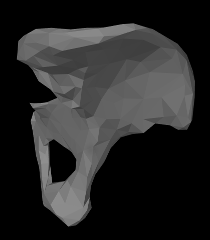
\includegraphics[]{images/hipBodyGray}&
   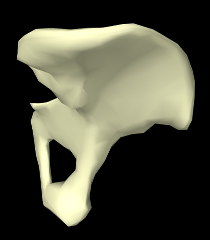
\includegraphics[]{images/hipBodySmooth}&
   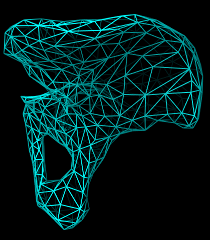
\includegraphics[]{images/hipBodyEdges}\\
 \else
   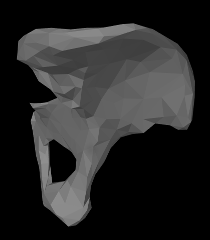
\includegraphics[width=2in]{images/hipBodyGray}&
   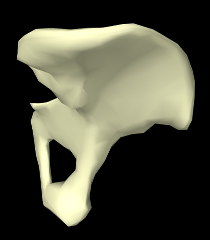
\includegraphics[width=2in]{images/hipBodySmooth}&
   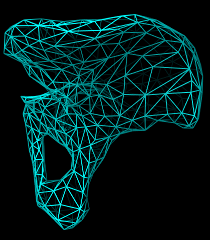
\includegraphics[width=2in]{images/hipBodyEdges}\\
 \fi
\end{tabular}
\end{center}
\caption{Different rendering settings for a rigid body hip mesh
showing the default (left), smooth rendering with a lighter color
(center), and wireframe (right).}
\label{HipRendering:fig}
\end{figure}

Properties can also be set in code, usually during the {\tt build()}
method. Typically this is done using a static method of the
\javaclass[maspack.render]{RenderProps} class that has the form
%
\begin{lstlisting}[]
  RenderProps.setXXX (comp, value)
\end{lstlisting}
%
where {\tt XXX} is the property name, {\tt comp} is the component for
which the property should be set, and {\tt value} is the desired
value. Some examples are shown in Figure \ref{HipRendering:fig} for a
rigid body hip representation with a fairly coarse mesh.  The
left image shows the default rendering, using a gray color and flat
shading. The center image shows a lighter color and smooth shading,
which could be set by the following code fragment:
%
\begin{lstlisting}[]
import maspack.render.*;
import maspack.render.Renderer.*;
  ...

  RigidBody hipBody;
  ...

  RenderProps.setFaceColor (hipBody, new Color (255, 255, 204));
  RenderProps.setShading (hipBody, Shading.SMOOTH);
\end{lstlisting}
%
Finally, the right image shows the body rendered as a wire
frame, which can by done by setting {\sf faceStyle} to {\tt NONE}
and {\sf drawEdges} to {\tt true}:
\begin{lstlisting}[]
  RenderProps.setFaceStyle (hip, FaceStyle.NONE);
  RenderProps.setDrawEdges (hip, true);
  RenderProps.setEdgeWidth (hip, 2);
  RenderProps.setEdgeColor (hip, Color.CYAN);
\end{lstlisting}
%

Render properties can also be set in higher level model components,
from which their values will be inherited by lower level components
that have not explicitly set their own values. For example, setting
the {\sf faceColor} render property in the {\tt MechModel} will
automatically set the face color for all subcomponents which have not
explicitly set {\sf faceColor}. More details on render properties are
given in Section \ref{RenderProperties:sec}.

\begin{figure}[h]
\begin{center}
\begin{tabular}{cc}
 \iflatexml
   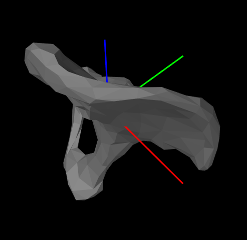
\includegraphics[]{images/hipBodyLineAxes}&
   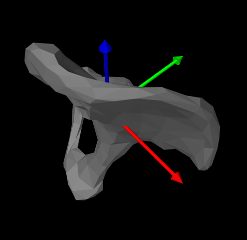
\includegraphics[]{images/hipBodyArrowAxes}\\
 \else
   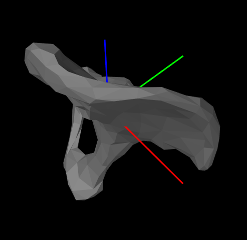
\includegraphics[width=2.5in]{images/hipBodyLineAxes}&
   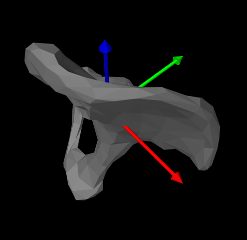
\includegraphics[width=2.5in]{images/hipBodyArrowAxes}\\
 \fi
\end{tabular}
\end{center}
\caption{Rigid body axes rendered with {\sf axisDrawStyle}
set to {\tt LINE} (left) and {\tt ARROW} (right).}
\label{AxisRendering:fig}
\end{figure}

In addition to mesh rendering, it is often useful to draw a rigid
body's coordinate frame, which can be done using its {\sf axisLength}
and {\sf axisDrawStyle} properties. Setting {\sf axisLength} to a
positive value will cause the body's three coordinate axes to be
drawn, with the indicated length, with the $x$, $y$ and $z$ axes
colored red, green, and blue, respectively. The {\tt axisDrawStyle}
property controls how the axes are rendered (Figure
\ref{AxisRendering:fig}). It has the type
\javaclass[maspack.render]{Renderer\$AxisDrawStyle}, and can
be set to the following values:
%
\begin{description}

\item[OFF]\mbox{}

Axes are not rendered.

\item[LINE]\mbox{}

Axes are rendered as simple red-green-blue lines,
with a width given by the joint's {\sf lineWidth} rendering property.

\item[ARROW]\mbox{}

Axes are rendered as solid red-green-blue arrows.

\end{description}
%

As with the rendering proprieties, the {\sf axisLength} and {\sf
axisDrawStyle} properties can be managed either interactively in the
GUI (by selecting the body, right clicking and choosing {\sf Edit
properties ...}), or in code, using the following methods:
% method table
\begin{lstlisting}[]
  double getAxisLength()
  void setAxisLength (double len)

  AxisDrawStyle getAxisDrawStyle()
  void setAxisDrawStyle (AxisDrawStyle style)
\end{lstlisting}
%

\subsection{Multiple meshes}
\label{rigidBodyMultipleMeshes:sec}

A {\tt RigidBody} may contain multiple meshes, which can be useful for
various reasons:

\begin{itemize}

\item It may be desirable to use different meshes for collision
detection, inertia computation, and visual presentation;

\item Different render properties can be set for different mesh
components, allowing the body to be rendered in a more versatile way;

\item Different mesh components can be selected individually.

\end{itemize}

Each rigid body mesh is encapsulated inside a
\javaclass[\mech]{RigidMeshComp} component, which is in turn stored in
a subcomponent list called {\tt meshes}. Meshes do not need to be
instances of \javaclass[maspack.geometry]{PolygonalMesh}; instead,
they can be any instance of \javaclass[maspack.geometry]{MeshBase},
including \javaclass[maspack.geometry]{PointMesh} and
\javaclass[maspack.geometry]{PolylineMesh}.

\begin{sideblock}
The default surface mesh, returned by {\tt getSurfaceMesh()}, is also
stored inside a {\tt RigidMeshComp} in the {\tt meshes} list. By
default, the surface mesh is the first mesh in the list, but is
otherwise defined to be the first mesh in {\tt meshes} which is also
an instance of {\tt PolygonalMesh}. The {\tt RigidMeshComp} containing
the surface mesh can be obtained using the method {\tt
getSurfaceMeshComp()}.
\end{sideblock}

A {\tt RigidMeshComp} contains a number of properties that control how
the mesh is displayed and interacts with its rigid body:

\begin{description}

\item[renderProps]\mbox{}

Render properties controlling how the mesh is
rendered (see Section \ref{RenderProperties:sec}).

\item[hasMass]\mbox{} 

A boolean, which if {\tt true} means that the mesh
will contribute to the body's inertia when the {\sf inertiaMethod}
is either {\tt MASS} or {\tt DENSITY}. The default value is {\tt true}.

\item[massDistribution]\mbox{} 

An enumerated type defined by
\javaclass[maspack.geometry]{MassDistribution} which specifies how the
mesh's inertia contribution is determined for a given mass.  {\tt
VOLUME}, {\tt AREA}, {\tt LENGTH}, and {\tt POINT} indicate,
respectively, that the mass is distributed evenly over the mesh's
volume, area (faces), length (edges), or points. The default value is
determined by the mesh type: {\tt VOLUME} for a closed {\tt
PolygonalMesh}, {\tt AREA} for an open {\tt PolygonalMesh}, {\tt
LENGTH} for a {\tt PolylineMesh}, and {\tt POINT} for a {\tt
PointMesh}. Applications can specify an alternate value providing the
mesh has the features to support it. Specifying {\tt DEFAULT} will
restore the default value.

\item[isCollidable]\mbox{} 

A boolean, which if {\tt true}, and if the mesh is a
{\tt PolygonalMesh}, means that the mesh will take part in collision
and wrapping interactions (Chapter \ref{ContactAndCollision:sec} and
Section \ref{GeneralSurfaceWrapping:sec}). The default value is {\tt true},
and the get/set accessors have the names {\tt isCollidable()} and
{\tt setIsCollidable()}.

\item[volume]\mbox{} 

A double whose value is the volume of the mesh.  If the
mesh is a {\tt PolygonalMesh}, this is the value returned by its
\javamethod[maspack.geometry.PolygonalMesh]{computeVolume()} method.
Otherwise, the volume is 0, unless
\javamethodAlt{\mech.RigidMeshComp.setVolume(double)}{setVolume(vol)} is
used to explicitly set a non-zero volume value.

\item[mass]\mbox{} 

A double whose default value is the product of the {\sf
density} and {\sf volume} properties. Otherwise,
if {\sf mass} has been explicitly set using
\javamethodAlt{\mech.RigidMeshComp.setMass(double)}{setMass(mass)},
the value is the explicit mass.

\item[density]\mbox{}

A double whose default value is the rigid body's
density.  Otherwise, if {\sf density} has been explicitly set using
\javamethodAlt{\mech.RigidMeshComp.setDensity(double)}{setDensity(density)},
the value is the explicit density, or if {\sf mass} has been explicitly
set using
\javamethodAlt{\mech.RigidMeshComp.setMass(double)}{setMass(mass)}, the
value is the explicit {\sf mass} divided by {\sf volume}.

\end{description}

Note that by default, the {\sf density} of a {\tt RigidMeshComp} is
simply the {\sf density} setting for the rigid body, and the {\sf
mass} is this times the {\sf volume}. However, it is possible to set
either an explicit mass or a density value that will override
this. (Also, explicitly setting a mass will unset any explicit
density, and explicitly setting the density will unset any explicit
mass.)

When the {\sf inertiaMethod} of the rigid body is either {\tt MASS} or
{\tt DENSITY}, then its inertia is computed from the sum of all the
inertias $\M_k$ of the component meshes $k$ for which {\sf hasMass} is
{\tt true}. Each $\M_k$ is computed by the mesh's
\javamethodAlt{maspack.geometry.MeshBase.createInertia(double,)}%
{createInertia(mass,massDistribution)} method,
using the {\sf mass} and {\sf massDistribution} properties of
its {\tt RigidMeshComp}.

\begin{sideblock}
When forming the body inertia from the inertia components of
individual meshes, no attempt is made to account for mesh overlap.  If
this is important, the meshes themselves should be modified in advance
so that they do not overlap, perhaps by using the CSG primitives
described in Section \ref{CSG:sec}.
\end{sideblock}

Instances of {\tt RigidMeshComp} can be created directly, using
constructions such as
%
\begin{lstlisting}[]
  PolygonalMesh mesh;

  ... initialize mesh ...

  RigidMeshComp mcomp = new RigidMeshComp (mesh);
\end{lstlisting}
%
or
%
\begin{lstlisting}[]
  RigidMeshComp mcomp = new RigidMeshComp ("meshName");
  mcomp.setMesh (mesh);
\end{lstlisting}
%
after which they can be added or removed from the {\tt meshes} list
using the methods
% method table
\begin{lstlisting}[]
  void addMeshComp (RigidMeshComp mcomp)
  void addMeshComp (RigidMeshComp mcomp, int idx)
  int numMeshComps()
  boolean removeMeshComp (RigidMeshComp mcomp)
  boolean removeMeshComp (String name)
  void clearMeshComps()
\end{lstlisting}
%
It is also possible to add meshes directly to the {\tt meshes} list,
using the methods
% method table
\begin{lstlisting}[]
  RigidMeshComp addMesh (MeshBase mesh)
  RigidMeshComp addMesh (MeshBase mesh, boolean hasMass, boolean collidable)
\end{lstlisting}
%
each of which creates a {\tt RigidMeshComp}, adds it to the mesh list,
and returns it.  The second method also specifies the values of the
{\sf hasMass} and {\sf collidable} properties (both of which are {\tt
true} by default).

\iflatexml
\subsection{Example: a composite rigid body}
\fi

\begin{figure}[ht]
\begin{center}
\iflatexml
 \includegraphics[]{images/RigidCompositeBody}
\else
 \includegraphics[width=3.75in]{images/RigidCompositeBody}
\fi
\end{center}
\caption{{\tt RigidCompositeBody} loaded into ArtiSynth and run for 0.75 seconds.
The ball on the right falls less because it has a lower
density than the rest of the body.}
\label{RigidCompositeBody:fig}
\end{figure}

\iflatexml
\else
\subsection{Example: a composite rigid body}
\fi

An example of constructing a rigid body from multiple meshes is
defined in
%
\begin{verbatim}
  artisynth.demos.tutorial.RigidCompositeBody
\end{verbatim}
%
This uses three meshes to construct a rigid
body whose shape resembles a dumbbell. The code, with the include
files omitted, is listed below:
\lstset{numbers=left}
\iflatexml
%% Hack: latexml lstinputlisting doesn't handle firstline correctly
\lstset{firstnumber={-14}}
\lstinputlisting[firstline=1]{../../src/artisynth/demos/tutorial/RigidCompositeBody.java}
\lstset{firstnumber={1}}
\else
\lstinputlisting[firstline=16]{../../src/artisynth/demos/tutorial/RigidCompositeBody.java}
\fi
\lstset{numbers=none}

As in the previous examples, the {\tt build()} method starts by
creating a {\tt MechModel} (lines 6-7). Three different meshes
(two balls and an axis) are then constructed at lines 10-15,
using {\tt MeshFactory} methods (Section \ref{Meshes:sec})
and transforming each result to an appropriate position/orientation with
respect to the body's coordinate frame.

The body itself is constructed at lines 18-24. Its default density is
set to 10, and its frame damping (Section \ref{RigidBodyDamping:sec})
is also set to 10 (the previous rigid body example in Section 
\ref{RigidBodySpringExample:sec} relied on spring damping to dissipate energy).
The meshes are added using
\javamethod*[\mech.RigidBody]{addMesh()},
which allocates and returns a 
\javaclass[\mech]{RigidMeshComp}. For the ball meshes,
these are saved in {\tt bcomp1} and {\tt bcomp2} and used later to
adjust density and/or render properties.

Lines 27-34 create a simple linear spring, connected to a fixed point
{\tt p0} and a marker {\tt mkr}. The marker is created and attached to
the body by the {\tt MechModel} method
\javamethod*[\mech.MechModel]{addFrameMarkerWorld(,)}, which places the
marker at a known position in world coordinates.  The spring is
created using an \javaclass[\mech]{AxialSpring} constructor that
accepts a name, along with stiffness, damping, and rest length
parameters to specify a
\javaclass[artisynth.core.materials]{LinearAxialMaterial}.

At line 37, {\tt bcomp1} is used to set the density of {\tt ball1} to
8. Since this is less than the default body density, the inertia
component of {\tt ball1} will be lighter than that of {\tt ball2}.
Finally, render properties are set at lines 41-45. This includes
setting the default face colors for the body and for each ball.

To run this example in ArtiSynth, select {\sf All demos > tutorial >
RigidCompositeBody} from the {\sf Models} menu. The model should load
and initially appear as in Figure \ref{RigidCompositeBody:fig}.
Running the model (Section \ref{LoadingAndRunning:sec}) will cause the
rigid body to fall and swing about under gravity, with the right ball
({\tt ball1}) not falling as far because it has less density.

\section{Mesh components}
\label{MeshComponents:sec}

ArtiSynth models frequently incorporate 3D mesh geometry, as defined
by the geometry classes \javaclass[maspack.geometry]{PolygonalMesh},
\javaclass[maspack.geometry]{PolylineMesh}, and
\javaclass[maspack.geometry]{PointMesh} described in Section
\ref{Meshes:sec}. Within a model, these basic classes are typically
enclosed within container components that are subclasses of
\javaclass[artisynth.core.mechmodels]{MeshComponent}. Commonly
used instances of these include

\begin{description}

\item[\protect{\javaclass[\mech]{RigidMeshComp}}]\mbox{}

Introduced in Section \ref{rigidBodyMultipleMeshes:sec}, these contain
the mesh geometry for rigid bodies, and are stored in a rigid body
subcomponent list named {\tt meshes}. Their mesh vertex positions
are fixed with respect to their body's coordinate frame.

\item[\protect{\javaclass[\fem]{FemMeshComp}}]\mbox{}

Contain mesh geometry associated with finite element models (Chapter
\ref{FEMModels:sec}), including surfaces meshes and embedded mesh
geometry, and are stored in a subcomponent list of the FEM model
named {\tt meshes}. Their mesh vertex positions change as the FEM model
deforms.

\item[\protect{\javaclass[\fem]{SkinMeshBody}}]\mbox{}

Described in detail in Chapter \ref{skinning:sec}, these describe
``skin'' geometry that encloses both rigid bodies and/or FEM models.
Their mesh vertex positions change as the underlying bodies move and
deform. Skinning meshes may be placed anywhere, but are typically
stored in the {\tt meshBodies} component list of a {\tt MechModel}.

\item[\protect{\javaclass[\mech]{FixedMeshBody}}]\mbox{}

Described further below, these store arbitrary mesh geometry
(polygonal, polyline, and point) and provide (like rigid bodies) a
rigid coordinate frame that allows the mesh to be positioned and
oriented arbitrarily. As their name suggests, their mesh vertex
positions are fixed with respect to this coordinate frame. Fixed body
meshes may be placed anywhere, but are typically stored in the {\tt
meshBodies} component list of a {\tt MechModel}.

\end{description}

\subsection{Fixed mesh bodies}
\label{FixedMeshBodies:sec}

As mentioned above, \javaclass[\mech]{FixedMeshBody} can be used for
placing arbitrary mesh geometry within an ArtiSynth model.  These mesh
bodies are non-dynamic: they do not interact or collide with other
model components, and they function primarily as 3D graphical
objects. They can be created from primary mesh components using
constructors such as:
%
\begin{methodtable}{0.5}{0.5}
\midline
%
\methodentry
{\mech .FixedMeshBody.FixedMeshBody(MeshBase)}%
{FixedMeshBody (MeshBase mesh)}%
{Create an unnamed body containing a specified mesh.}%
%
\methodentry
{\mech .FixedMeshBody.FixedMeshBody(String,MeshBase)}%
{FixedMeshBody (String name, MeshBase mesh)}%
{Create a named body containing a specified mesh.}%
%
\midline
\end{methodtable}
%
It should be noted that the primary meshes are not copied and are
instead stored by reference, and so any subsequent changes to them
will be reflected in the mesh body. As with rigid bodies, fixed mesh
bodies contain a coordinate frame, or {\it pose}, that describes the
position and orientation of the body with respect to world
coordinates. Methods to control the pose include:
%
\begin{methodtable}{0.5}{0.5}
\midline
%
\methodentry
{\mech .FixedMeshBody.getPose()}%
{RigidTransform3d getPose()}%
{Returns the pose of the body (with respect to world).}%
%
\methodentry
{\mech .FixedMeshBody.setPose()}%
{void setPose (RigidTransform3d XFrameToWorld)}%
{Sets the pose of the body.}%
\methodspace{0.5em}
%
\methodentry
{\mech .FixedMeshBody.getPosition()}%
{Point3d getPosition()}%
{Returns the body position (pose translation component).}%
%
\methodentry
{\mech .FixedMeshBody.setPosition()}%
{void setPosition (Point3d pos)}%
{Sets the body position.}%
\methodspace{0.5em}
%
\methodentry
{\mech .FixedMeshBody.getOrientation()}%
{AxisAngle getOrientation()}%
{Returns the body orientation (pose rotation component).}%
%
\methodentry
{\mech .FixedMeshBody.setOrientation()}%
{void setOrientation (AxisAngle axisAng)}%
{Sets the body orientation.}%
%
\midline
\end{methodtable}
%
Once created, a canonical place for storing mesh bodies is the {\tt
MechModel} component list {\tt meshBodies}. Methods for
maintaining this list include:
%
\begin{methodtable}{0.5}{0.5}
\midline
%
\methodentry{\mech .MechModel.meshBodies()}%
{ComponentListView<MeshComponent> meshBodies()}%
{Returns the {\tt meshBodies} list.}%
%
\methodentry{\mech .MechModel.addMeshBody()}%
{void addMeshBody (MeshComponent mcomp)}%
{Adds {\tt mcomp} to {\tt meshBodies}.}%
%
\methodentry{\mech .MechModel.removeMeshBody()}%
{boolean removeMeshBody (MeshComponent mcomp)}%
{Removes {\tt mcomp} from {\tt meshBodies}.}%
%
\methodentry{\mech .MechModel.clearMeshBodies()}%
{void clearMeshBodies()}%
{Clears the {\tt meshBodies} list.}%
%
\midline
\end{methodtable}
%
Meshes used for instantiating fixed mesh bodies are typically read
from files (Section \ref{MeshFileIO:sec}), but can also be created
using factory methods (Section \ref{MeshCreation:sec}).  As an
example, the following code fragment creates a torus mesh using a
factory method, set its pose, and then adds it to a {\tt MechModel}:
%
\begin{lstlisting}[]
   MechModel mech;
   ...
   PolygonalMesh mesh = MeshFactory.createTorus (
      /*rmajor=*/1.0, /*rminor=*/0.2, /*nmajor=*/32, /*nminor=*/10);
   FixedMeshBody mbody = new FixedMeshBody ("torus", mesh);
   mbody.setPose (
      new RigidTransform3d (/*xyz=*/0,0,0, /*rpy=*/0,0,Math.toRadians(90)));
   mech.addMeshBody (mbody);
\end{lstlisting}
%

Rendering of mesh bodies is controlled using the same properties
described in Section \ref{rigidBodyRendering:sec} for rigid bodies,
including the {\sf renderProps} subproperties {\sf faceColor}, {\sf
shading}, {\sf alpha}, {\sf faceStyle}, and {\sf drawEdges}, and the
properties {\sf axisLength} and {\sf axisDrawStyle} for displaying a
body's coordinate frame.

\subsection{Example: adding mesh bodies to MechModel}
\label{FixedMeshesExample:sec}

\begin{figure}[h]
\begin{center}
\iflatexml
 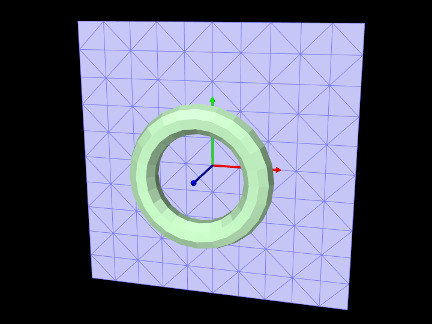
\includegraphics[]{images/FixedMeshes}
\else
 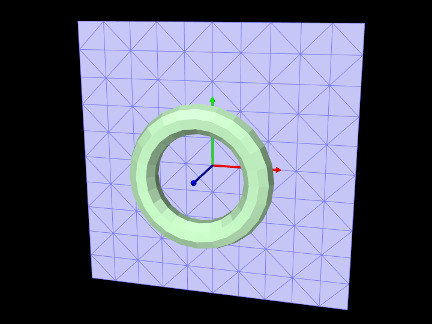
\includegraphics[width=3.75in]{images/FixedMeshes}
\fi
\end{center}
\caption{FixedMeshes model loaded into ArtiSynth.}
\label{FixedMeshes:fig}
\end{figure}

An simple application that creates a pair of fixed meshes and adds
them to a {\tt MechModel} is defined in
%
\begin{verbatim}
  artisynth.demos.tutorial.FixedMeshes
\end{verbatim}
%
The {\tt build()} method for this is shown below:
\lstset{numbers=left}
\iflatexml
%% Hack: latexml lstinputlisting doesn't handle firstline correctly
\lstset{firstnumber={-18}}
\lstinputlisting[firstline=1,lastline=42]{../../src/artisynth/demos/tutorial/FixedMeshes.java}
\lstset{firstnumber={1}}
\else
\lstinputlisting[firstline=20,lastline=61]{../../src/artisynth/demos/tutorial/FixedMeshes.java}
\fi
\lstset{numbers=none}
%
After creating a {\tt MechModel} (lines 3-4), a torus shaped mesh is
imported from the file {\tt data/torus\_9\_24.obj} (lines 8-16). As
described in Section \ref{PathFinder:sec}, the {\tt RootModel} method
{\tt getSourceRelativePath()} is used to locate this file relative to
the model's source folder. The file path is used in the {\tt
PolygonalMesh} constructor, which is enclosed within a {\tt try/catch}
block to handle possible I/O exceptions. Once imported, the mesh is
used to instantiate a {\tt FixedMeshBody} named {\tt "torus"} which is
added to the {\tt MechModel} (lines 18-19).

Another mesh, representing a square, is created with a factory method
and used to instantiate a mesh body named {\tt "square"} (lines
22-26). The factory method specifies both the size and triangle
density of the mesh in the $x$-$y$ plane. Once created, the square's
pose is set to a 90 degree rotation about the $x$ axis and a
translation of 0.5 along $y$ (lines 28-29).

Rendering properties are set at lines 33-41. The torus is made pale
green by setting it face color; the coordinate frame for the square is
made visible as solid arrows using the {\tt axisLength} and {\tt
axisDrawStyle} properties; and the square is made blue gray, with its
edges made visible and drawn using a darker color, and its face style
set to {\tt FRONT\_AND\_BACK} so that it's visible from either side.

To run this example in ArtiSynth, select {\sf All demos > tutorial >
FixedMeshes} from the {\sf Models} menu. The model should load and
initially appear as in Figure \ref{FixedMeshes:fig}.

\section{Joints and connectors}
\label{JointsAndConnectors:sec}

In a typical mechanical model, many of the rigid bodies are
interconnected, either using spring-type components that exert binding
forces on the bodies, or through joints and connectors that enforce
the connection using hard constraints. This section describes the
latter. While the discussion focuses on rigid bodies, joints and
connectors can be used more generally with any body that implements
the \javaclass[artisynth.core.mechmodels]{ConnectableBody}
interface. In particular, this allows joints to also interconnect
finite element models, as described in Section \ref{FEMJoints:sec}.

\subsection{Joints and coordinate frames}
\label{JointsAndFrames:sec}

Consider two rigid bodies A and B. The pose of body B with respect to
body A can be described by the 6 DOF rigid transform $\T_{BA}$.  If A
and B are unconnected, $\T_{BA}$ may assume any possible value and has
a full six degrees of freedom. A {\it joint} between A and B
constrains the set of poses that are possible between the two bodies
and reduces the degrees of freedom available to $\T_{BA}$.  For ease
of use, the constraining action of a joint is described with respect
to a pair of local coordinate frames C and D that are connected to
frames A and B, respectively, by auxiliary transformations.  This
allows joints to be placed at locations that do not correspond
directly to frames A or B.

\begin{figure}[ht]
\begin{center}
 \iflatexml
   \includegraphics[width=2in]{images/jointExample}
 \else
   \includegraphics[width=2in]{images/jointExample}
 \fi
\end{center}
\caption{Coordinate frames D and C for a hinge joint.}
\label{jointExample:fig}
\end{figure}

The joint frames C and D move with respect to each other as the joint
moves. The allowed joint motions therefore correspond to the allowed
values of the {\it joint transform} $\T_{CD}$.  Although both frames
typically move with their attached bodies, D is considered the {\it
base} frame and C the {\it motion} frame (this is because when a joint
is used to connect a single body to ground, body B is set to {\tt
null} and the world frame takes its place).  As an example of a
joint's constraining effect, consider a hinge joint (Figure
\ref{jointExample:fig}), which allows C to move with respect to D {\it only} by
rotating about the $z$ axis while the origins of C and D remain
coincident. Other motions are prohibited. If we let $\theta$ describe
the counter-clockwise rotation angle of C about the $z$ axis, then
$\T_{CD}$ should always have the form
%
\begin{equation}
\T_{CD} = \matl
\cos(\theta) & -\sin(\theta) & 0 & 0 \\
\sin(\theta) &  \cos(\theta) & 0 & 0 \\
0 & 0 & 1 & 0 \\
0 & 0 & 0 & 1 
\matr.
\end{equation}
%

\begin{figure}[ht]
\begin{center}
 \iflatexml
   \includegraphics[width=3.74in]{images/jointBodyFrames}
 \else
   \includegraphics[width=3.74in]{images/jointBodyFrames}
 \fi
\end{center}
\caption{Transforms connecting joint coordinate frames C and D with
rigid bodies A and B.}
\label{jointBodyFrames:fig}
\end{figure}

When a joint is attached to bodies A and B, frame C is fixed to body A
and frame D is fixed to body B. Except in special cases, the joint
frames C and D are not coincident with the body frames A
and B.  Instead, they are located relative to A and B by the
transforms $\T_{CA}$ and $\T_{DB}$, respectively
(Figure \ref{jointBodyFrames:fig}). Since $\T_{CA}$ and $\T_{DB}$ are
both fixed, the joint constraints on $\T_{CD}$ constrain the relative
poses of A and B, with $\T_{AB}$ determined from
%
\begin{equation}
\T_{AB} = \T_{DB} \, \T_{CD} \, \T_{CA}^{-1}.
\label{jointPose:eqn}
\end{equation}
%
(See Section \ref{RigidTransforms:sec} for a discussion of determining
transforms between related coordinate frames).

\subsection{Joint coordinates, constraints, and errors}
\label{JointCoordinates:sec}

Each different joint and connector type restricts the motion between
two bodies to $M$ degrees of freedom, for some $M < 6$.  Sometimes,
the joint also defines a set of $M$ coordinates that parameterize
these $M$ DOFs. For example, the hinge joint described above is
parameterized by $\theta$. Other examples are given in
Section \ref{JointTypes:sec}: a 2 DOF cylindrical has coordinates $z$
and $\theta$, a 3 DOF gimbal joint is parameterized by the
roll-pitch-yaw angles $\theta$, $\phi$, and $\psi$, etc.  When
$\T_{CD} = \I$ (where $\I$ is the identity transform), the coordinates
are usually all equal to zero, and the joint is said to be in the {\it
zero state}.

As explained in Section \ref{PhysicsSimulation:sec}, ArtiSynth uses a
full coordinate formulation for dynamic simulation. That means that
instead of using joint coordinates to describe system state, it uses
the combined full coordinates $\q$ of all dynamic components. For
example, a model consisting of a single rigid body connected to ground
by a hinge joint will have 6 DOF (corresponding to the 6 DOF of the
body), rather than the 1 DOF implied by the hinge joint.  The DOF
restrictions imposed by the joints are then enforced by a set of
linearized constraint relationships
%
\begin{equation}
\G(\q) \u = \g, \qquad \N(\q) \u \ge \n
\label{constraints2:eqn}
\end{equation}
%
that restrict the body velocities $\u$ computed at each simulation
step, usually by solving an MLCP like (\ref{KKTvelocity:eqn}). As
explained in Section \ref{PhysicsSimulation:sec}, the right side
vectors $\g$ and $\n$ in (\ref{constraints2:eqn}) contain time
derivative terms, which for simplicity much of the following
presentation will assume to be 0.

Each joint contributes its own set of constraint equations to
(\ref{constraints2:eqn}). Typically these take the form of {\it
bilateral}, or equality, constraints
%
\begin{equation}
\G_\text{J}(\q) \u = 0
\label{bilateralG:eqn}
\end{equation}
%
which are added to the system's global bilateral constraint matrix
$\G$. $\G_\text{J}$ contains $6 - M$ rows providing $6 - M$ individual
constraints $\G_k$.
During simulation, these give rise to $6 - M$ constraint
forces (corresponding to $\Blam$ in (\ref{impulsesToForces:eqn}))
which enforce the constraints.

In some cases, the joint also maintains {\it unilateral}, or inequality
constraints, to keep $\T_{CD}$ out of inadmissible regions. These take
the form
%
\begin{equation}
\N_\text{J}(\q) \u \ge 0
\label{unilateralN:eqn}
\end{equation}
%
and are added to the system's global unilateral constraint matrix
$\N$.  They give rise to constraint forces corresponding to $\Bthe$ in
(\ref{impulsesToForces:eqn}). A common use of unilateral constraints
is to enforce range limits of the joint coordinates (Section
\ref{coordinateLimitsAndLocking:sec}), such as
%
\begin{equation}
\theta_{\text{min}} \le \theta \le \theta_{\text{max}}.
\end{equation}
%
A specific unilateral constraint is added to $\N_\text{J}$ only when
$\T_{CD}$ is on or within the boundary of the inadmissible region
associated with that constraint. The constraint is then said to be
{\it engaged}. The combined number of bilateral and engaged unilateral
constraints for a particular joint should not exceed 6; otherwise, the
joint would be overconstrained.

Joint coordinates, when supported for a particular joint, can be both
read and set. Setting a coordinate causes the joint transform
$\T_{CD}$ to change. To accommodate this, the system adjusts the poses
of one or both bodies connected to the joint, along with adjacent
bodies connected to them, with preference given to bodies that are not
attached to ``ground''.  However, if this is done during simulation,
and particularly if one or both of the bodies connected to the joint
are moving dynamically, the results will be unpredictable and will
likely conflict with the simulation.

Joint coordinates are also often exported as properties. For example,
the
\javaclass[artisynth.core.mechmodels]{HingeJoint}
class (Section \ref{JointTypes:sec}) exports its $\theta$ coordinate
as the property {\sf theta}, which can be accessed in the GUI, or via
the accessor methods
% method table
\begin{lstlisting}[]
  double getTheta()          // get theta in degrees

  void setTheta (double deg) // set theta in degrees
\end{lstlisting}
%

Since joint constraints are generally nonlinear, their linearized
enforcement at the velocity level by (\ref{constraints2:eqn}) will
usually produce small errors as the simulation proceeds.  These errors
are reduced using a position correction step described in
Section \ref{JointConstraints:sec} and \cite{lloyd2012artisynth}.
Errors can also be caused by joint compliance
(Section \ref{JointCompliance:sec}).  Both effects mean that the joint
transform $\T_{CD}$ may deviate from the allowed values dictated by
the joint type. In ArtiSynth, this is accounted for by introducing an
additional {\it constraint} frame G between D and C
(Figure \ref{jointFrames:fig}).  G is computed to be the nearest frame
to C that lies exactly in the joint constraint space. $\T_{GD}$ is
therefore a valid joint transform, $\T_{GC}$ accommodates the error,
and the whole joint transform is given by the composition
%
\begin{equation}
\T_{CD} = \T_{GD} \; \T_{CG}.
\end{equation}
%
If there is no compliance or joint error, then frames G and C are
identical, $\T_{CG} = \I$, and $\T_{CD} = \T_{GD}$.  Because $\T_{CG}$
describes the joint error, we sometimes refer to it as $\T_{err}
= \T_{CG}$.

\begin{figure}[ht]
\begin{center}
 \iflatexml
   \includegraphics[width=3.5in]{images/jointFrames}
 \else
   \includegraphics[width=3.5in]{images/jointFrames}
 \fi
\end{center}
\caption{2D schematic showing the joint frames D and C, along with
the intermediate frame G that accounts for numeric error
and complaint motion.}
\label{jointFrames:fig}
\end{figure}

\subsection{Creating joints}
\label{CreatingJoints:sec}

Joint and connector components in ArtiSynth are both derived from the
superclass
\javaclass[artisynth.core.mechmodels]{BodyConnector},
with joints being further derived from
\javaclass[artisynth.core.mechmodels]{JointBase},
which provides support for coordinates.  Some of the commonly used
joints and connectors are described in Section
\ref{JointTypes:sec}.

An application creates a joint by constructing it and adding it to a {\tt
MechModel}. For this, two things need to be specified:
%
\begin{enumerate}
\item The bodies A and B being connected;

\item The initial locations of the C and D frames.	
\end{enumerate}
%
For the second item, it is often more convenient to specify C and D in world
coordinates, i.e., as $\T_{CW}$ and $\T_{DW}$, and then determine $\T_{CA}$ and
$\T_{DB}$ from
%
\begin{align}
\T_{CA} & = \T_{AW}^{-1} \; \T_{CW} \\
\T_{DB} & = \T_{BW}^{-1} \; \T_{DW},
\end{align}
%
where $\T_{AW}$ and $\T_{BW}$ are the current poses of A and B.

Many joints have constructors of the form
%
\begin{lstlisting}[]
  XXXJoint (bodyA, bodyB, TDW)
\end{lstlisting}
%
which specifies {\it only} $\T_{DW}$ and the bodies A and B. The constructor
then computes $\T_{CW}$ from
%
\begin{equation}
\T_{CW} = \T_{BW} \T_{CD},
\label{initialTCW:eqn}
\end{equation}
%
where $\T_{CD}$ is the joint's initial $\T_{CD}$ value returned by
\javamethod*[\mech.BodyConnector]{getCurrentTCD()}. For joints
with coordinates, the initial $\T_{CD}$ is determined from the initial
coordinate values (which are usually 0). Typically (but not always), the
initial $\T_{CD}$ is also the identity, so that $\T_{CW} = \T_{DW}$.

After the joint is created, it should be added to the system's {\tt
MechModel} using
\javamethod[artisynth.core.mechmodels.MechModel]{addBodyConnector()}, as
shown in the following code fragment:
%
\begin{lstlisting}[]
   MechModel mech; 
   RigidBody bodyA, bodyB;
   RigidTransform3d TDW;

   ... initialize mech, bodyA, bodyB, and TDW ...
   
   HingeJoint joint = new HingeJoint (bodyA, bodyB, TDW);
   mech.addBodyConnector (joint);
\end{lstlisting}
%

Joints usually offer a number of other constructors that let its world
location and body relationships to be specified in different
ways. These may include:
%
\begin{lstlisting}[]
  XXXJoint (bodyA, TCA, bodyB, TDB)

  XXXJoint (bodyA, bodyB, TCW, TDW)
\end{lstlisting}
%
The first, which is restricted to rigid bodies, allows the application
to explicitly specify transforms $\T_{CA}$ and $\T_{DB}$ connecting
frames C and D to the body frames A and B, and is useful when
$\T_{CA}$ and $\T_{DB}$ are explicitly known, or the initial value of
$\T_{CD}$ is {\it not} the identity. Likewise, the second constructor
allows $\T_{CW}$ and $\T_{DW}$ to be explicitly specified, with
$\T_{CD} \ne \I$ if $\T_{CW} \ne \T_{DW}$.  For instance, suppose
$\T_{CD}$ and $\T_{DW}$ are both known. Then we can use the
relationship
%
\begin{equation}
\T_{CW} = \T_{DW} \, \T_{CD}
\end{equation}
%
to create the joint as in the following code fragment:
%
\begin{lstlisting}[]
   MechModel mech;
   RigidBody bodyA, bodyB;
   RigidTransform3d TDW, TCD;

   ... initialize mech, bodyA, bodyB, TDW, and TCD ...

   // compute TCW:
   RigidTransform3d TCW = new RigidTransform3d();
   TCW.mul (TDW, TCD);
   HingeJoint joint = new HingeJoint (bodyA, bodyB, TCW, TDW);
   mech.addBodyConnector (joint);
\end{lstlisting}
%

As an alternative to specifying $\T_{DW}$ or its equivalents, some
joint types provide constructors that let the application locate
specific joint features. These may be easier to use in some cases. For
instance, \javaclass[artisynth.core.mechmodels]{HingeJoint} provides a
constructor
% method table
\begin{lstlisting}[]
   HingeJoint (bodyA, bodyB, originD, zaxis)
\end{lstlisting}
%
that specifies origin of D and its $z$ axis (which is the rotation
axis), with the remaining orientation of D aligned as closely as
possible with the world.
\javaclass[artisynth.core.mechmodels]{SphericalJoint} provides a
constructor
% method table
\begin{lstlisting}[]
   SphericalJoint (bodyA, bodyB, originD)
\end{lstlisting}
%
that specifies origin of D and aligns its orientation with the world.
Users should consult the source code or API documentation for specific
joints to see what special constructors may be available.

It is also possible to use a joint to connect a single body to ``ground''
(i.e., the world frame). When this is done, the body in question is always {\tt
bodyA}, and {\tt bodyB} is {\tt null}. Most joints provide a constructor of the
form
%
\begin{lstlisting}[]
  XXXJoint (bodyA, TDW)
\end{lstlisting}
%
which allows this to be done explicitly. Alternatively, most joint
constructors which supply body B will allow this to be specified as
{\tt null}, so that body A will be connected to ground by default.

\begin{sideblock}
When using joints to build an articulated structure, the usual convention is
for {\tt bodyA} to be on the distal, or ``outer'', side of the joint and for
{\tt bodyB} to be on the proximal, or ``inner side.
\end{sideblock}

Finally, it is also possible to create a joint using its default constructor
and attach it to the bodies {\it afterward}, using the various {\tt setBodies()}
methods:
%
\begin{methodtable}{0.67}{0.33}
\midline
%
\methodentry
{\mech.BodyConnector.setBodies(ConnectableBody,ConnectableBody,)}%
{void setBodies (ConnectableBody bodyA, ConnectableBody bodyB,\brh
RigidTransform3d TDW)}%
{Set A and B given TDW.}%
%
\methodentry
{\mech.BodyConnector.setBodies(ConnectableBody,ConnectableBody,,)}%
{void setBodies (ConnectableBody bodyA, ConnectableBody bodyB,\brh
RigidTransform3d TCW, RigidTransform3d TDW)}%
{Set A and B given TCW and TDW.}%
%
\methodentry
{\mech.BodyConnector.setBodies(RigidBody,,,)}%
{void setBodies (RigidBody bodyA, RigidTransform3d TCA,\brh
RigidBody bodyB, RigidTransform3d TDB)}%
{Set A and B given TCA and TDB.}%
%
\methodentry
{\mech.BodyConnector.setBodies(ConnectableBody,FrameAttachment,,)}%
{void setBodies (ConnectableBody bodyA, FrameAttachment attachmentA,\brh
ConnectableBody bodyB, FrameAttachment attachmentB)}%
{Set A and B with custom attachments.}%
\methodspace{0.5em}%
\methodentry
{\mech.BodyConnector.setBodyA(ConnectableBody,RigidTransform3d)}%
{void setBodyA (ConnectableBody bodyA, RigidTransform3d TCW)}%
{Set A given TCW.}%
%
\methodentry
{\mech.BodyConnector.setBodyA(ConnectableBody,FrameAttachment)}%
{void setBodyA (ConnectableBody bodyA, FrameAttachment attachmentA)}%
{Set A with custom attachment.}%
%
\methodentry
{\mech.BodyConnector.setBodyB(ConnectableBody,RigidTransform3d)}%
{void setBodyB (ConnectableBody bodyB, RigidTransform3d TDW)}%
{Set B given TDW.}%
%
\methodentry
{\mech.BodyConnector.setBodyB(ConnectableBody,FrameAttachment)}%
{void setBodyB (ConnectableBody bodyB, FrameAttachment attachmentB)}%
{Set B with custom attachment.}%
%
%\brh
\midline
\end{methodtable}
%
As with the constructors, {\tt TDW} and {\tt TCW} give the locations of D and C
in world coordinates, and if {\tt TCW} is needed but not specified, it is
computed per equation (\ref{initialTCW:eqn}). {\tt bodyB} can also be given as
{\tt null}, which will cause body A to be attached to ground.  The methods
specifying {\tt FrameAttachment}s allow for situations where special attachment
types are needed, such as when connecting joints to finite element models
(Section \ref{FEMJoints:sec}).  The {\tt setBodyA()} and {\tt setBodyB()}
methods connect body A (or body B) while leaving body B (or body A) alone, and
are useful when it is necessary to set (or reset) only one body connection.

The following example creates a {\tt HingeJoint} using {\tt setBodies()}:
%
\begin{lstlisting}[]
   RigidTransform3d TDW;
   ConnectableBody bodyA, bodyB;
   ...
   HingeJoint joint = new HingeJoint();
   joint.setBodies (bodyA, bodyB, TDW);
   mech.addBodyConnector (joint);
\end{lstlisting}
%
A more complicated, but exactly equivalent, version using {\tt setBodyA()} and
{\tt setBodyB()} is given by
%
\begin{lstlisting}[]
   RigidTransform3d TCD = new RigidTransform3d();
   RigidTransform3d TCW = new RigidTransform3d();

   HingeJoint joint = new HingeJoint();
   joint.getCurrentTCD (TCD);
   TCW.mul (TDW, TCD);
   joint.setBodyA (bodyA, TCW);
   joint.setBodyB (bodyB, TDW);
   mech.addBodyConnector (joint);
\end{lstlisting}
%
One reason for using {\tt setBodies()} is that it allows the joint transform
$\T_{CD}$ to be modified (by setting coordinate values) {\it before} {\tt
setBodies()} is called; this is discussed further in
Section \ref{workingWithCoordinates:sec}.

\subsection{Working with coordinates}
\label{workingWithCoordinates:sec}

As mentioned in Section \ref{JointCoordinates:sec}, some joints
support coordinates that parameterize the valid motions within the
joint transform $\T_{CD}$. All such joints are subclasses of
\javaclass[artisynth.core.mechmodels]{JointBase},
which provides some generic methods for querying and setting
coordinate values ({\tt JointBase} is in turn a subclass of
\javaclass[artisynth.core.mechmodels]{BodyConnector}).

The number of coordinates is returned by the method {\tt
numCoordinates()}; if this returns 0, then coordinates are not
supported. Each coordinate has an index in the range $0 \ldots M-1$,
where $M$ is the number of coordinates. Coordinate values can be
queried or set using the following methods:
% method table
\begin{lstlisting}[]
  getCoordinate (int idx)               // get coordinate value with index idx
  getCoordinates (VectorNd coords)      // get all coordinates values

  setCoordinate (int idx, double value) // set coordinate value with index idx
  setCoordinates (VectorNd values)      // set all coordinates values
\end{lstlisting}
%

Specific joint types usually also provide names for their joint
coordinates, along with integer constants describing their indices
and methods for accessing their values. For example,
\javaclass[artisynth.core.mechmodels]{CylindricalJoint}
supports two coordinates, $z$ and $\theta$, along with
the following:
%
\begin{lstlisting}[]
  // coordinate indices
  static final int Z_IDX = 0;
  static final int THETA_IDX = 1;

  // set/get z value and range
  double getZ()
  void setZ (double z)

  // set/get theta value and range in degrees
  double getTheta()
  void setTheta (double theta)
\end{lstlisting}
%
The coordinate values are also exported as the properties {\sf z} and
{\sf theta}, allowing them to be set in the GUI. For convenience,
particularly in GUI applications, the properties and methods for
controlling specific angular coordinates generally use degrees instead
of radians.

As discussed in Section \ref{JointCoordinates:sec}, unlike in some
multibody simulation systems (such as OpenSim), joint coordinates are
{\it not} fundamental quantities that describe system state. As such,
then, coordinates can usually only be set in specific circumstances
that avoid simulation conflicts. In general, when joint coordinates
are set, the system adjusts the poses of one or both bodies connected
to this joint, along with adjacent bodies connected to them, with
preference given to bodies that are not attached to ``ground''.
However, if this is done during simulation, and particularly if one or
both of the bodies connected to the joint are moving dynamically, the
results will be unpredictable and will likely conflict with the
simulation.

If a joint has been created with its default constructor and not yet
attached to any bodies, then setting joint values will simply set the
joint transform $\T_{CD}$. This can be useful in situations where one
needs to initialize a joint's $\T_{CD}$ to a non-identity value
corresponding to a particular set of joint coordinates:
%
\begin{lstlisting}[]
  RigidTransform3d TDW; // known location for D frame
  double z, theta; // desired initial coordinate values
  ...
  CylindricalJoint joint = new CylindricalJoint();
  joint.setZ (z);
  joint.setTheta (thetaDeg);
  joint.setBodies (bodyA, bodyB, TDW);
\end{lstlisting}
%
This can also be done in vector form:
%
\begin{lstlisting}[]
  RigidTransform3d TDW; // known location for D frame
  VectorNd coordValues; // desired initial coordinate values
  ...
  CylindricalJoint joint = new CylindricalJoint();
  joint.setCoordinates (coordValues);
  joint.setBodies (bodyA, bodyB, TDW);
\end{lstlisting}
%
In either of these cases, {\tt setBodies()} will not use $\T_{CD}
= \I$ but instead use the value determined by the initial coordinate
values.

To determine the $\T_{CD}$ corresponding to a particular set of
coordinates, one may use the method
% method table
\begin{lstlisting}[]
  void coordinatesToTCD (RigidTransform3d TCD, VectorNd coords)
\end{lstlisting}
%

In some cases, within a model's {\tt build()} method, one may wish to
set initial coordinates {\it after} a joint has been attached to its
bodies, in order to move those bodies (along with the bodies attached
to them) into an initial configuration without having to explicitly
calculate the poses from the joint coordinates. As mentioned
above, the system will make a decision about which attached bodies are
most ``free'' and adjust their poses accordingly. This is done in the
example of the next section.

\subsection{Coordinate limits and locking}
\label{coordinateLimitsAndLocking:sec}

It is possible to set limits on a joint coordinate's range, and also
to lock a coordinate in place at its current value.

When a joint coordinate hits either an upper or lower range limit, a
unilateral constraint is invoked to prevent it from violating the
limit, and remains engaged until the joint moves away from the
limit. Each range constraint that is engaged reduces the number of
joint DOFs by one.

By default, joint range limits are usually disabled (i.e., they are
set to $(-\inf, \inf)$). They can be queried and set, for a given
joint with index {\tt idx}, using the methods:
% method table
\begin{lstlisting}[]
  DoubleInterval getCoordinateRange (int idx)	
  double getMinCoordinate (int idx)
  double getMaxCoordinate (int idx)
  void setCoordinateRange (idx, DoubleInterval rng)
\end{lstlisting}
%
where range limits for angular coordinates are specified in
radians. For convenience, the following methods are also provided
which use degrees instead of radians for angular coordinates:
% method table
\begin{lstlisting}[]
  DoubleInterval getCoordinateRangeDeg (int idx)
  double getMinCoordinateDeg (int idx)
  double getMaxCoordinateDeg (int idx)
  void setCoordinateRangeDeg (idx, DoubleInterval rng)
\end{lstlisting}
%
Range checking can be disabled by setting the range to
$(-\inf, \inf)$, or by specifying {\tt rng} as {\tt null}, which
implicitly does the same thing.

\begin{sideblock}
Ranges for angular coordinates are not limited to $\pm 180^\circ$ but
can instead be set to larger values; the joint will continue to wrap
until the limit is reached.
\end{sideblock}

Joint coordinates can also be {\it locked}, so that they hold their
current value and don't move. A joint is locked using a bilateral
constraint that prevents motion in either direction and reduces the
joint's DOF count by one.  The following methods are available for
querying or setting a coordinate's locked status:
% method table
\begin{lstlisting}[]
  boolean isLocked (int idx)	
  void setLocked (int idx, boolean locked)
\end{lstlisting}
%

As with coordinate values, specific joint types usually provide
methods for controlling the ranges and locking status of individual
coordinates, with ranges for angular coordinates specified in degrees
instead of radians.  For example,
\javaclass[artisynth.core.mechmodels]{CylindricalJoint}
supplies the methods
% method table
\begin{lstlisting}[]
  // set/get z range
  DoubleInterval getZRange()
  void setZRange (double min, double max)

  // control z locking
  boolean isZLocked()
  void setZLocked (boolean locked)

  // set/get theta range in degrees
  DoubleInterval getThetaRange()
  void setThetaRange (double min, double max)
  void setThetaRange (DoubleInterval rng)

  // control theta locking
  boolean isThetaLocked()
  void setThetaLocked (boolean locked)
\end{lstlisting}
%
The range and locking information is also exported as the properties
{\sf zRange}, {\sf thetaRange}, {\sf zLocked}, and {\sf thetaLocked},
allowing them to be set in the GUI.

\subsection{Example: a simple hinge joint}
\label{RigidBodyJoint:sec}

\begin{figure}[ht]
\begin{center}
\iflatexml
 \includegraphics[]{images/RigidBodyJoint}
\else
 \includegraphics[width=3.75in]{images/RigidBodyJoint}
\fi
\end{center}
\caption{RigidBodyJoint model loaded into ArtiSynth.}
\label{RigidBodyJoint:fig}
\end{figure}

A simple model showing two rigid bodies connected by
a joint is defined in
%
\begin{verbatim}
  artisynth.demos.tutorial.RigidBodyJoint
\end{verbatim}
%

The build method for this model is given below:
\lstset{numbers=left}
\begin{lstlisting}[]
   public void build (String[] args) {

      // create MechModel and add to RootModel
      mech = new MechModel ("mech");
      mech.setGravity (0, 0, -98);
      mech.setFrameDamping (1.0);
      mech.setRotaryDamping (4.0);
      addModel (mech);

      PolygonalMesh mesh;  // bodies will be defined using a mesh

      // create first body and set its pose
      mesh = MeshFactory.createRoundedBox (lenx1, leny1, lenz1, /*nslices=*/8);
      RigidTransform3d TMB = 
         new RigidTransform3d (0, 0, 0, /*axisAng=*/1, 1, 1, 2*Math.PI/3);
      mesh.transform (TMB);
      bodyB = RigidBody.createFromMesh ("bodyB", mesh, /*density=*/0.2, 1.0);
      bodyB.setPose (new RigidTransform3d (0, 0, 1.5*lenx1, 1, 0, 0, Math.PI/2));
      bodyB.setDynamic (false);

      // create second body and set its pose
      mesh = MeshFactory.createRoundedCylinder (
         leny2/2, lenx2, /*nslices=*/16, /*nsegs=*/1, /*flatBottom=*/false);
      mesh.transform (TMB);
      bodyA = RigidBody.createFromMesh ("bodyA", mesh, 0.2, 1.0);
      bodyA.setPose (new RigidTransform3d (
                        (lenx1+lenx2)/2, 0, 1.5*lenx1, 1, 0, 0, Math.PI/2));

      // create the joint      
      RigidTransform3d TDW = 
         new RigidTransform3d (lenx1/2, 0, 1.5*lenx1, 1, 0, 0, Math.PI/2);
      HingeJoint joint = new HingeJoint (bodyA, bodyB, TDW);

      // add components to the mech model
      mech.addRigidBody (bodyB);
      mech.addRigidBody (bodyA);
      mech.addBodyConnector (joint);

      joint.setTheta (35);  // set joint position

      // set render properties for components
      RenderProps.setFaceColor (joint, Color.BLUE);
      joint.setShaftLength (4);
      joint.setShaftRadius (0.2);
   }
\end{lstlisting}
\lstset{numbers=none}

A {\tt MechModel} is created as usual at line 4. However, in this
example, we also set some parameters for it:
\javamethod*[artisynth.core.mechmodels.MechModel]{setGravity()} is
used to set the gravity acceleration vector to $(0, 0, -98)^T$ instead
of the default value of $(0, 0, -9.8)^T$, and the {\tt frameDamping}
and {\tt rotaryDamping} properties (Section
\ref{RigidBodyDamping:sec}) are set to provide appropriate damping.

Each of the two rigid bodies are created from a mesh and a density.
The meshes themselves are created using the factory methods
\javamethod*[maspack.geometry]{MeshFactory.createRoundedBox(,,,)} and
\javamethod*[maspack.geometry]{MeshFactory.createRoundedCylinder(,,,,)}
(lines 13 and 22), and then
\javamethod*[artisynth.core.mechmodels]{RigidBody.createFromMesh(,,,)} is
used to turn these into rigid bodies with a density of 0.2 (lines 17
and 25). The pose of the two bodies is set using {\tt
RigidTransform3d} objects created with x, y, z translation and
axis-angle orientation values (lines 18 and 26).

The hinge joint is implemented using
\javaclass[artisynth.core.mechmodels]{HingeJoint}, which is
constructed at line 32 with the joint coordinate frame D being located
in world coordinates by {\tt TDW} 
as described in Section \ref{CreatingJoints:sec}.

Once the joint is created and added to the {\tt MechModel}, the method
\javamethod*[artisynth.core.mechmodels.HingeJoint]{setTheta()} is
used to explicitly set the joint parameter to 35 degrees. The joint
transform $\T_{CD}$ is then set appropriately and {\tt bodyA} is moved
to accommodate this ({\tt bodyA} being chosen since it is the most
free to move).

Finally, joint rendering properties are set starting at line 42. We
render the joint as a cylindrical shaft about the rotation axis, using
its {\sf shaftLength} and {\sf shaftRadius} properties. Joint
rendering is discussed in more detail in
Section \ref{RenderingJoints:sec}).

To run this example in ArtiSynth, select {\sf All demos > tutorial >
RigidBodyJoint} from the {\sf Models} menu. The model should load and
initially appear as in Figure \ref{RigidBodyJoint:fig}.  Running the
model (Section \ref{LoadingAndRunning:sec}) will cause {\tt bodyA} to
fall and swing under gravity.

\subsection{Constraint forces}

During each simulation solve step, the joint velocity constraints
described by (\ref{bilateralG:eqn}) and (\ref{unilateralN:eqn}) are
enforced by bilateral and unilateral constraint forces $\f_g$ and
$\f_n$:
%
\begin{equation}
\f_g = \G_\text{J}^T \Blam_J, \quad \f_n = \N_\text{J}^T \Bthe_J.
\end{equation}
%
Here, $\f_g$ and $\f_n$ are spatial forces (or {\it wrenches}, Section
\ref{SpatialVelocitiesAndForces:sec}) acting in the joint coordinate
frame C, and $\Blam_J$ and $\Bthe_J$ are the Lagrange multipliers
computed as part of the mechanical system solve (see
(\ref{KKTvelocity:eqn}) and (\ref{impulsesToForces:eqn})).  The sizes
of $\Blam_J$ and $\Bthe_J$ equal the number of bilateral and {\it
engaged} unilateral constraints in the joint; these numbers can be
queried for a particular joint using the methods
\javamethod[artisynth.core.mechmodels.BodyConnector]{numBilateralConstraints()}
and
\javamethod[artisynth.core.mechmodels.BodyConnector]{%
numEngagedUnilateralConstraints()}.
(The number of engaged unilateral constraints may be less than the
total number of unilateral constraints; the latter may be queried with
\javamethod[artisynth.core.mechmodels.BodyConnector]{numUnilateralConstraints()},
while the total number of
constraints is returned by
\javamethod[artisynth.core.mechmodels.BodyConnector]{numConstraints()}.

Applications may sometimes need to query the current constraint force
values, typically from within a controller
or monitor (Section \ref{ControllersAndMonitors:sec}).
The Lagrange multipliers themselves may be obtained with
% method table
\begin{lstlisting}[]
  void getBilateralForces (VectorNd lam)

  void getUnilateralForces (VectorNd the)
\end{lstlisting}
%
which load the multipliers into {\tt lam} or {\tt the} and set their
sizes to the number of bilateral or engaged unilateral
constraints. Alternatively, one can retrieve the individual multiplier
for the constraint indexed by {\tt idx} using
% method table
\begin{lstlisting}[]
  double getConstraintForce (int idx);
\end{lstlisting}
%

Typically, it is more useful to find the spatial constraint forces
$\f_g$ and $\f_n$, which can be obtained with respect to frame C:
% method table
\begin{lstlisting}[]
  // place the forces in the wrench f
  void getBilateralForcesInC (Wrench f)
  void getUnilateralForcesInC (Wrench f)

  // convenience methods that allocate the wrench and return it
  Wrench getBilateralForcesInC();
  Wrench getUnilateralForcesInC();
\end{lstlisting}
%
If the attached bodies A and B are rigid bodies, it is also possible
to obtain the constraint wrenches experienced by those bodies:
% method table
\begin{lstlisting}[]
  // place the forces in the wrench f
  void getBilateralForcesInA (Wrench f)
  void getUnilateralForcesInA (Wrench f)
  void getBilateralForcesInB (Wrench f)
  void getUnilateralForcesInB (Wrench f)

  // convenience methods that allocate the wrench and return it
  Wrench getBilateralForcesInA();
  Wrench getUnilateralForcesInA();
  Wrench getBilateralForcesInB();
  Wrench getUnilateralForcesInB();
\end{lstlisting}
%
Constraint wrenches obtained for bodies A or B are given in world
coordinates, which is consistent with the forces reported by rigid
bodies via their {\tt getForce()} method. To orient the forces into
body coordinates, one may use the inverse of the rotation matrix $\R$
of the body's pose. For example:
%
\begin{lstlisting}[]
   RigidBody bodyA;

   // ... body A initialized, etc. ...

   Wrench force = joint.getBilateralForceInA();
   force.inverseTransform (bodyA.getPose().R);
\end{lstlisting}
%

\subsection{Compliance and regularization}
\label{JointCompliance:sec}

By default, the constraints used to implement joints and couplings are
treated as {\it hard}, so that the system tries to respect the
constraint conditions (\ref{constraints2:eqn}) as exactly as possible
as the simulation proceeds.  Sometimes, however, it is desirable to
introduce some ``softness'' into the constraints, whereby constraint
forces are determined as a linear function of their distance from the
constraint. Adding compliance also allows an application to {\it
regularize} a system of joint constraints that would otherwise be
overconstrained, as illustrated in Section \ref{FourBar:sec}.

To describe compliance precisely, consider the bilateral constraint
portion of the MLCP in (\ref{KKTvelocity:eqn}), which solves for the
updated system velocities $\u^{k+1}$ at each time step:
%
\begin{equation}
\matl
\hat\M^{k} & -\G^{T} \\
\G & 0
\matr
\matl
\u^{k+1} \\
\tilde\Blam
\matr
=
\matl
\M \u^{k} - h \hat\f^{k} \\
0
\matr.
\label{KKThard:eqn}
\end{equation}
%
Here $\G$ is the system's bilateral constraint matrix, $\tilde\Blam$
denotes the constraint impulses (from which the constraint forces
$\Blam$ can be determined by $\Blam = \tilde\Blam/h$), and for
simplicity we have assumed that $\G$ is constant and so the $\g$ term
on the lower right side is $0$.

Solving (\ref{KKThard:eqn}) results in constraint forces that satisfy
$\G \u^{k+1} = 0$ precisely, corresponding to hard constraints. To
implement soft constraints, start by defining a function $\Bphi(\q)$
that defines the {\it distances} from each constraint, where $\q$ is the
vector of system positions; these distances are
the local translational and rotational deviations from each
constraint's correct position and are discussed in more detail in
Section \ref{JointConstraints:sec}. Then assume that the constraint
forces are a linear function of these distances:
%
\begin{equation}
\Blam = -\C^{-1} \Bphi(\q),
\label{compliance:eqn}
\end{equation}
%
where $\C$ is a diagonal {\it compliance} matrix that is equivalent to
an inverse stiffness matrix. We also note that $\Bphi$ will be time
varying, and that we can approximate its change between time steps as
%
\begin{equation}
\Bphi^{k+1} \approx \Bphi^k + h \dot\Bphi^{k+1}, \quad \text{with}
\quad \dot\Bphi^{k+1} = \G \u^{k+1}.
\label{BphiApprox:eqn}
\end{equation}
%
Next, assume that in using (\ref{compliance:eqn}) to determine $\Blam$
for a particular time step, we use the {\it average} value of $\Bphi$
over the step, represented by $\bar\Bphi = (\Bphi^{k+1} + \Bphi^k)/2$.
Substituting this and (\ref{BphiApprox:eqn}) into
(\ref{compliance:eqn}), multiplying by $\C$, and rearranging yields:
%
\begin{equation}
\G \u^{k+1} + \frac{2 \C}{h} \Blam = -\frac{2}{h} \Bphi^k.
\end{equation}
%
Then noting that $\tilde\Blam = h \Blam$, we obtain
a revised form of (\ref{KKThard:eqn}),
%
\begin{equation}
\matl
\hat\M^{k} & -\G^{T} \\
\G & 2 \C /h^2 
\matr
\matl
\u^{k+1} \\
\tilde\Blam
\matr
=
\matl
\M \u^{k} - h \hat\f^{k} \\
- 2 \Bphi^k/h
\matr,
\label{KKTsoft:eqn}
\end{equation}
%
in the which the zeros in the matrix and right hand side have been
replaced by compliance terms.
The resulting constraint behavior is different from that of
(\ref{KKThard:eqn}) in two important ways:

\begin{enumerate}

\item The joint now allows 6 DOF, with motion along the constrained directions
limited by restoring spring constants given by the reciprocals of the
diagonal entries of $\C$.

\item If $\C$ has no zero diagonal entries, then the system
(\ref{KKTsoft:eqn}) is {\it regularized} by the $2 \C/h^2$ term in the
lower right matrix block. This means that the matrix is always
non-singular, even if $\G$ is rank deficient, and so compliance offers
a way to handle overconstrained models, as discussed further in
Section \ref{FourBar:sec}.

\end{enumerate}

Unilateral constraints can be regularized using the same approach,
with a distance function defined such that $\Bphi(\q) \le 0$.  

The reason for specifying soft constraints using compliance instead of
stiffness is that by setting $\C = 0$ we can easily handle the case of
{\it infinite} stiffness where the constraints are strictly enforced.
The ArtiSynth compliance implementation uses a slightly more complex
version of (\ref{KKTsoft:eqn}) that accounts for non-constant $\G$ and
also allows for a damping term $-\D \dot\Bphi$, where $\D$ is again a
diagonal matrix.  For more details, see \cite{lacoursiere2007ghosts}
and \cite{servin2006interactive}.

When using compliance, damping is often needed for stability, and, in
the case of unilateral constraints, to prevent ``bouncing''.  A good
choice for damping is usually {\it critical damping}, which is
discussed further below.

Any joint which is a subclass of
\javaclass[artisynth.core.mechmodels]{BodyConnector} allows
individual compliance values $C_i$ and damping values $D_i$ to be set
for each of the joint's $i$ constraints. These values comprise the
diagonal entries in the compliance and damping matrices $\C$ and $\D$,
and can be queried and set using the methods
% method table
\begin{lstlisting}[]
  VectorNd getCompliance()
  void setCompliance (VectorNd compliance)

  VectorNd getDamping()
  void setCompliance (VectorNd damping)
\end{lstlisting}
%
The vectors supplied to the above {\tt set} methods contain the
requested compliance or damping values. If their size $n$ is less than
{\tt numConstraints()}, then compliance or damping will be set for the
first $n$ constraints.  Damping for a specific constraint only has an
effect if the compliance for that constraint is nonzero.

What compliance and damping values should be specified? Compliance is
usually relatively easy to figure out. Each of the joint's individual
constraints $i$ corresponds to a row in its bilateral constraint matrix
$\G_\text{J}$ or unilateral constraint matrix $\N_\text{J}$, and represents a
specific 6 DOF direction along which the spatial velocity
$\hat\v_{CD}$ (of frame C with respect to D) is restricted (more
details on this are given in Section \ref{JointConstraints:sec}).
Each of these constraint directions is usually predominantly linear or
rotational; specific descriptions for the constraints of different
joints are provided in Section \ref{JointTypes:sec}. To determine
compliance for a constraint $i$, estimate the typical force $f$ likely
to act along its direction, decide how much displacement $\delta q$
(translational or rotational) along that constraint is desirable, and
then set the compliance $C_i$ to the associated inverse stiffness:
%
\begin{equation}
C_k = \delta q/f.
\end{equation}
%
Once $C_k$ is determined, the damping $D_k$ can be estimated based on
the desired damping ratio $\zeta$, using the formula
%
\begin{equation}
D_k = 2 \zeta \sqrt{M/C_k}
\label{constraintDamping:eqn}
\end{equation}
%
where $M$ is total mass of the bodies attached to the joint.
Typically, the desired damping will be close to critical damping, for
which $\zeta = 1$.

Constraints associated with linear motion will typically require
different compliance values from those associated with rotation.  To
make this process easier, joint components allow the setting of
collective compliance values for their linear and rotary constraints,
using the methods
% method table
\begin{lstlisting}[]
  void setLinearCompliance (double c)
  double getLinearCompliance()

  void setRotaryCompliance (double c)
  double getRotaryCompliance()
\end{lstlisting}
%
The {\tt set()} methods will set a uniform compliance for all linear or
rotary constraints, except for unilateral constraints associated with
coordinate limits. At the same time, they will also set an {\it
automatically} computed critical damping value. Likewise, the {\tt
get()} methods query these linear or rotary constraints for uniform
compliance values (with the corresponding critical damping), and
return either that value, or -1 if it does not exist.

Most of the demonstration models for the joints described in
Section \ref{JointTypes:sec} allow these linear and rotary compliance
settings to be adjusted interactively using a control panel, enabling
users to experimentally gain a feel for their behavior.

To determine programmatically whether a particular constraint is linear
or rotary, one can use the joint method
% method table
\begin{lstlisting}[]
  VectorNi getConstraintFlags()
\end{lstlisting}
%
which returns a vector of information flags for all its constraints.
Linear and rotary constraints are indicated by the flags {\tt LINEAR}
and {\tt ROTARY}, defined in 
\javaclass[maspack.spatialmotion]{RigidBodyConstraint}.

\subsection{Example: an overconstrained linkage}
\label{FourBar:sec}

Situations may occasionally arise in which a model is {\it
overconstrained}, which means that the rows of the bilateral
constraint matrix $\G$ in (\ref{constraints2:eqn}) are not all
linearly dependent, or in other words, $\G$ does not have {\it full
row rank}. At present, the ArtiSynth solver has difficultly handling
overconstrained models, but these situations can often be handled by
adding a small amount of compliance to the
constraints. (Overconstraining is not a problem with unilateral
constraints $\N$, because of the way they are handled by the solver.)

One possible symptom of an overconstrained system is a error message
in the application's terminal output, such as
%
\begin{verbatim}
Pardiso: num perturbed pivots=12
\end{verbatim}

Overconstraining frequently occurs in closed-chain linkages, involving
loops in which a jointed sequence of links is connected back on
itself. Depending on how the constraints are configured and how
redundant they are, the system may still be able to move.  A classical
example is the {\it four-bar linkage}, a common version of which
consists of four links, or ``bars'', arranged as a parallelogram and
connected by hinge joints at the corners. One link is usually
connected to ground, and so the remaining three links together have 18
DOF, while the four hinge joints together remove 20 DOF,
overconstraining the system. However, the constraints are redundant in
such as way that the linkage still actually has 1 DOF.

\begin{figure}[ht]
\begin{center}
\iflatexml
 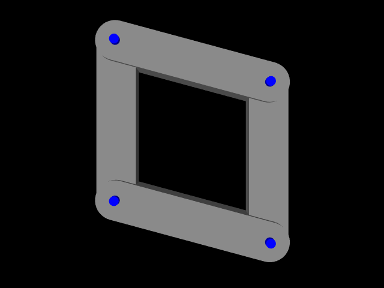
\includegraphics[]{images/FourBarLinkage}
\else
 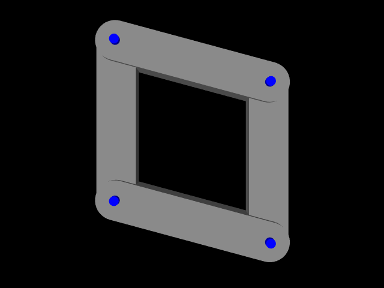
\includegraphics[width=3.75in]{images/FourBarLinkage}
\fi
\end{center}
\caption{FourBarLinkage model, several steps into the simulation.}
\label{FourBarLinkage:fig}
\end{figure}

To model a four-bar in ArtiSynth presently requires adding compliance
to the hinge joints. An example of this is defined by the demo program
%
\begin{verbatim}
  artisynth.demos.tutorial.FourBarLinkage
\end{verbatim}
%
shown in Figure \ref{FourBarLinkage:fig}.
The code for the {\tt build()} method and a couple of supporting
methods is given below:
\lstset{numbers=left}
\iflatexml
%% Hack: latexml lstinputlisting doesn't handle firstline correctly 
  \lstset{firstnumber={-25}}
  \lstinputlisting[firstline=1,lastline=73]{../../src/artisynth/demos/tutorial/FourBarLinkage.java}
  \lstset{firstnumber={1}}
\else
  \lstinputlisting[firstline=27,lastline=99]{../../src/artisynth/demos/tutorial/FourBarLinkage.java}
\fi
\lstset{numbers=none}
Two helper methods are used to construct the model: {\tt createLink()}
(lines 6-17), and {\tt createJoint()} (lines 23-36).  {\tt
createLink()} makes the individual rigid bodies used to build the
linkage: a mesh is produced defining the body's shape (a box with
rounded ends), and then passed to the
\javaclass[artisynth.core.mechmodels]{RigidBody}
{\tt createFromMesh()} method which creates the body and sets its
inertia according to a specified density. The body's pose is then set
so as to center it at $(x, 0, z)$ while rotating it about the $y$ axis
by the angle {\tt deg} (in degrees). The completed body is then added to the
{\tt MechModel} {\tt mech} and returned.

The second helper method, {\tt createJoint()}, connects two rigid
bodies ({\tt link0} and {\tt link1}) together using a {\tt
HingeJoint}. Because we know the location of the joint in
body-relative coordinates, it is easier to create the joint using the
transforms $\T_{CA}$ and $\T_{DB}$ instead of $\T_{DW}$: $\T_{CA}$
locates the joint at the top end of {\tt link0}, at $(0, 0, 0.5)$,
with the $z$ axis parallel to the body's $y$ axis, while $\T_{DB}$
similarly locates the joint at the bottom of {\tt link1}.  After the
joint is created and added to the {\tt MechModel}, its render
properties are set so that its axis drawn as a blue cylinder.

The {\tt build()} method itself begins by creating a {\tt MechModel}
and setting damping parameters for the rigid bodies (lines
40-43). Next, {\tt createLink()} is used to create and store the four
links (lines 46-50), and the left bar is attached to ground by making
it non-dynamic (line 52). The links are then connected together using
joints created by {\tt createJoint()} (lines 55-59). Finally, uniform
compliance and damping values are set for each of the joint's
bilateral constraints, using the {\tt setCompliance()} and {\tt
setDamping()} methods (lines 63-72). Values are set for the first five
constraints, since for a {\tt HingeJoint} these are the bilateral
constraints. The compliance value of $C = 10^{-6}$ was found
experimentally to be low enough so as to not cause noticeable
deflections in the joints. Given $C$ and an
average mass of around $M = 150$ for each link pair,
(\ref{constraintDamping:eqn}) suggests the damping factor of $D =
25000$. Note that for this example, very similar settings could be
achieved by simply calling
%
\begin{lstlisting}[]
  for (int i=0; i<joints.length; i++) {
     joints[i].setLinearCompliance (0.000001);
     joints[i].setRotaryCompliance (0.000001);
  }
\end{lstlisting}
%
In principle, we only need to set compliance for the constraints that
are redundant, but it can sometimes be difficult to determine exactly
which these are. Also, different values are often needed for linear
and rotary constraints; that is not necessary here because the
links have unit length and so the linear and rotary units have similar
scales.

\subsection{Rendering joints}
\label{RenderingJoints:sec}

Most joints provide a means to render themselves in order to provide a
graphical representation of their position and configuration.  Control
over this is achieved by setting various properties in the joint
component, including both specialized properties and the standard
render properties (Section \ref{RenderProperties:sec}) used by all
renderable components.

All joints which are subclasses of
\javaclass[artisynth.core.mechmodels]{JointBase} support rendering of
both their C and D coordinate frames, through the properties {\sf
drawFrameC}, {\sf drawFrameD}, and {\sf axisLength}.  The first two
properties are of the type
\javaclass[maspack.render]{Renderer\$AxisDrawStyle} (described
in detail in Section \ref{rigidBodyRendering:sec}), and can be set to
{\tt LINE} or {\tt ARROW} to enable the coordinate axes to be drawn
either as lines or solid arrows. The {\sf axisLength} property has
type {\tt double} and specifies the length with which the axes are
drawn. As with all properties, these properties can be set either in
the GUI, or in code using accessor methods supplied by the joint:
% method table
\begin{lstlisting}[]
  void setAxisLength (double l)
  double getAxisLength()

  void setDrawFrameC (AxisDrawStyle style)
  (AxisDrawStyle getDrawFrameC()

  void setDrawFrameD (AxisDrawStyle style)
  (AxisDrawStyle getDrawFrameD()
\end{lstlisting}
%

Another pair of properties used by several joints is {\sf shaftLength}
and {\sf shaftRadius}, which specify the length and radius used to
draw shaft or axis structures associated with the joint.  These are
rendered as solid cylinders, using the color indicated by the {\sf
faceColor} rendering property.  The default value of both properties
is 0; if {\sf shaftLength} is 0, then the structures are not drawn,
while if {\sf shaftRadius} is 0, a default value proportional to {\sf
shaftLength} is used. For example, to enable rendering of a blue shaft
along the rotation axis of a hinge joint, one may use the code
fragment
%
\begin{lstlisting}[]
  HingeJoint joint;
  ...

  joint.setShaftLength (0.5); // set shaft dimensions
  joint.setShaftRadius (0.05);
  RenderProps.setFaceColor (joint, Color.BLUE); // set the color
\end{lstlisting}
%
As another example, to enable rendering of a green ball about the
center of a spherical joint, one may use the fragment
%
\begin{lstlisting}[]
  SphericalJoint joint;
  ...

  joint.setJointRadius (0.02); // set the ball size
  RenderProps.setFaceColor (joint, Color.GREEN); // set the color
\end{lstlisting}
%

Specific joints may define additional properties to control how they
are rendered.

\section{Joint components}
\label{JointTypes:sec}

ArtiSynth supplies a number of basic joints and connectors in the package {\tt
artisynth.core.mechmodels}, the most common of which are described
here. 

Many of the descriptions are associated with a demonstration model,
named {\tt XXXJointDemo}, where {\tt XXX} is the joint type.  These
demos are located in the package {\tt artisynth.demos.mech}, and can
be loaded by selecting {\sf All demos > mech > XXXJointDemo} from the
{\sf Models} menu. When run, they can be interactively controlled,
using either the pull tool (see the section ``Pull Manipulation'' in
the \artisynthManual{uiguide}{ArtiSynth User Interface Guide}), or the
interactive control panel. The control panel allows the adjustment of
coordinate values and ranges (if supported), some of the render
properties, and the different {\sf compliance} and {\sf damping}
properties (Section \ref{JointCompliance:sec}).  One can inspect the
source code for each demo in its {\tt .java} file located in the
folder {\tt <ARTISYNTH\_HOME>/src/artisynth/demos/mech}.

\subsection{Hinge joint}
\label{HingeJoint:sec}

\begin{figure}[h]
\begin{center}
\begin{tabular}{c@{\hskip .5in}c}
 \iflatexml
   \includegraphics[width=2.333in]{images/hingeJoint}&
   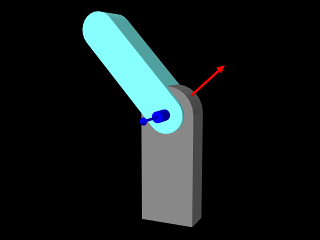
\includegraphics[width=3.1in]{images/HingeJointDemo}\\
 \else
   \includegraphics[width=1.75in]{images/hingeJoint}&
   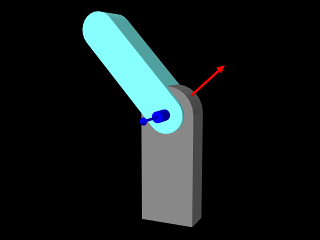
\includegraphics[width=2.333in]{images/HingeJointDemo}\\
 \fi
\end{tabular}
\end{center}
\caption{Coordinate frames (left) and demo model (right)
for the hinge joint.}
\label{HingeJoint:fig}
\end{figure}

The \javaclass[artisynth.core.mechmodels]{HingeJoint} 
(Figure \ref{HingeJoint:fig}) is a 1 DOF joint that
constrains motion between frames C and D to a simple rotation about
the $z$ axis of D.  It implements six constraints and one coordinate
$\theta$ (Table \ref{HingeConstraints:tbl}), to which the joint transform
$\T_{CD}$ is related by
%
\begin{equation*}
\T_{CD} = \matl
\cos(\theta) & -\sin(\theta) & 0 & 0 \\
\sin(\theta) &  \cos(\theta) & 0 & 0 \\
0 & 0 & 1 & 0 \\
0 & 0 & 0 & 1 
\matr.
\end{equation*}
%
The value and ranges for $\theta$ are exported by the properties {\sf
theta} and {\sf thetaRange}, and the $\theta$ coordinate index is
defined by the constant {\tt THETA\_IDX}.  For rendering, the
properties {\sf shaftLength} and {\sf shaftRadius} control the size of
a shaft drawn about the rotation axis, using the {\sf faceColor}
rendering property.  A demo is provided by \\ {\tt
artisynth.demos.mech.HingeJointDemo}.

In addition to the standard constructors described in
Section \ref{CreatingJoints:sec},
% method table
\begin{lstlisting}[]
  HingeJoint (bodyA, bodyB, originD, zaxis)
\end{lstlisting}
%
creates a hinge joint with a specified origin and $z$ axis direction
for frame D (in world coordinates), and frames C and D coincident.

\begin{table}[h]
\centering
\begin{tabular}{|l|l|l|}
\hline
Index & type/name & description \\
\hline
0 & bilateral & restricts translation along $x$ \\
1 & bilateral & restricts translation along $y$ \\
2 & bilateral & restricts translation along $z$ \\
3 & bilateral & restricts rotation about $x$ \\
4 & bilateral & restricts rotation about $y$ \\
5 & unilataral & enforces limits on $\theta$ \\
\hline
\hline
0 & $\theta$ & counter-clockwise rotation of $C$ about the $z$ axis \\
\hline
\end{tabular}
\caption{Constraints (top) and coordinates (bottom) for the hinge joint.}
\label{HingeConstraints:tbl}
\end{table}

\subsection{Slider joint}

\begin{figure}[h]
\begin{center}
\begin{tabular}{c@{\hskip .5in}c}
 \iflatexml
   \includegraphics[width=2.333in]{images/sliderJoint}&
   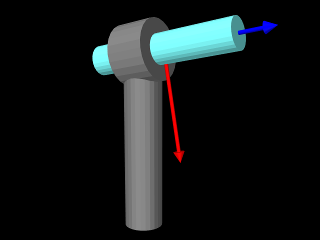
\includegraphics[width=3.1in]{images/SliderJointDemo}\\
 \else
   \includegraphics[width=1.75in]{images/sliderJoint}&
   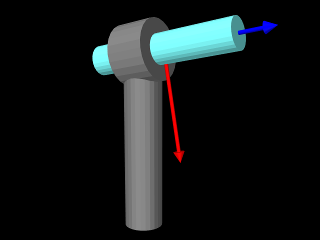
\includegraphics[width=2.333in]{images/SliderJointDemo}\\
 \fi
\end{tabular}
\end{center}
\caption{Coordinate frames (left) and demo model (right)
for the slider joint.}
\label{SliderJoint:fig}
\end{figure}

The \javaclass[artisynth.core.mechmodels]{SliderJoint} 
(Figure \ref{SliderJoint:fig}) is a 1 DOF joint
that constrains motion between frames C and D to a simple translation
along the $z$ axis of D.  It implements six constraints and one
coordinate $z$ (Table \ref{SliderConstraints:tbl}), to which the joint
transform $\T_{CD}$ is related by
%
\begin{equation*}
\T_{CD} = \matl
1 & 0 & 0 & 0 \\
0 & 1 & 0 & 0 \\
0 & 0 & 1 & z \\
0 & 0 & 0 & 1 
\matr.
\end{equation*}
%\
The value and ranges for $z$ are exported by the properties {\sf z}
and {\sf zRange}, and the $z$ coordinate index is defined by the
constant {\tt Z\_IDX}.  For rendering, the properties {\sf
shaftLength} and {\sf shaftRadius} control the size of a shaft drawn
about the sliding axis, using the {\sf faceColor} rendering property.
A demo is provided by {\tt artisynth.demos.mech.SliderJointDemo}.

In addition to the standard constructors described in
Section \ref{CreatingJoints:sec},
% method table
\begin{lstlisting}[]
  SliderJoint (bodyA, bodyB, originD, zaxis)
\end{lstlisting}
%
creates a slider joint with a specified origin and $z$ axis direction
for frame D (in world coordinates), and frames C and D coincident.

\begin{table}[h]
\centering
\begin{tabular}{|l|l|l|}
\hline
Index & type/name & description \\
\hline
0 & bilateral & restricts translation along $x$ \\
1 & bilateral & restricts translation along $y$ \\
2 & bilateral & restricts rotation about $x$ \\
3 & bilateral & restricts rotation about $y$ \\
4 & bilateral & restricts rotation about $z$ \\
5 & unilataral & enforces limits on the $z$ coordinate \\
\hline
\hline
0 & $z$ & translation of $C$ along the $z$ axis \\
\hline
\end{tabular}
\caption{Constraints (top) and coordinates (bottom) for the slider joint.}
\label{SliderConstraints:tbl}
\end{table}

\subsection{Cylindrical joint}

\begin{figure}[h]
\begin{center}
\begin{tabular}{c@{\hskip .5in}c}
 \iflatexml
   \includegraphics[width=2.333in]{images/cylindricalJoint}&
   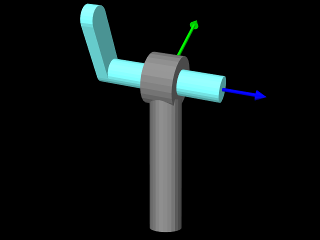
\includegraphics[width=3.1in]{images/CylindricalJointDemo}\\
 \else
   \includegraphics[width=1.75in]{images/cylindricalJoint}&
   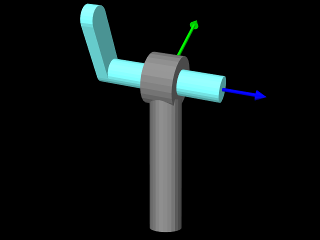
\includegraphics[width=2.333in]{images/CylindricalJointDemo}\\
 \fi
\end{tabular}
\end{center}
\caption{Coordinate frames (left) and demo model (right)
for the cylindrical joint.}
\label{CylindricalJoint:fig}
\end{figure}

The \javaclass[artisynth.core.mechmodels]{CylindricalJoint} 
(Figure \ref{CylindricalJoint:fig}) is a 2 DOF
joint that constrains motion between frames C and D to translation and
rotation along and about the $z$ axis of D.  It implements six
constraints and two coordinates $z$ and $\theta$
(Table \ref{CylindricalConstraints:tbl}), to which the joint transform
$\T_{CD}$ is related by
%
\begin{equation*}
\T_{CD} = \matl
\cos(\theta) & -\sin(\theta) & 0 & 0 \\
\sin(\theta) &  \cos(\theta) & 0 & 0 \\
0 & 0 & 1 & z \\
0 & 0 & 0 & 1 
\matr.
\end{equation*}
%\
The value and ranges for $z$ and $\theta$ are exported by the
properties {\sf z}, {\sf theta}, {\sf zRange} and {\sf thetaRange},
and the coordinate indices are defined by the constants {\tt Z\_IDX}
and {\tt THETA\_IDX}. For rendering, the properties {\sf shaftLength}
and {\sf shaftRadius} control the size of a shaft drawn about the
sliding/rotation axis, using the {\sf faceColor} rendering property.
A demo is provided by {\tt artisynth.demos.mech.CylindricalJointDemo}.

In addition to the standard constructors described in
Section \ref{CreatingJoints:sec},
% method table
\begin{lstlisting}[]
  CylindricalJoint (bodyA, bodyB, originD, zaxis)
\end{lstlisting}
%
creates a cylindrical joint with a specified origin and $z$ axis direction
for frame D (in world coordinates), and frames C and D coincident.

\begin{table}[h]
\centering
\begin{tabular}{|l|l|l|}
\hline
Index & type/name & description \\
\hline
0 & bilateral & restricts translation along $x$ \\
1 & bilateral & restricts translation along $y$ \\
2 & bilateral & restricts rotation about $x$ \\
3 & bilateral & restricts rotation about $y$ \\
4 & unilataral & enforces limits on the $z$ coordinate \\
5 & unilataral & enforces limits on the $\theta$ coordinate \\
\hline
\hline
0 & $z$ & translation of $C$ along the $z$ axis \\
1 & $\theta$ & rotation of $C$ about the $z$ axis \\
\hline
\end{tabular}
\caption{Constraints (top) and coordinates (bottom) for the cylindrical joint.}
\label{CylindricalConstraints:tbl}
\end{table}

\subsection{Slotted hinge joint}
\label{SlottedHingeJoint:sec}

\begin{figure}[h]
\begin{center}
\begin{tabular}{c@{\hskip .5in}c}
 \iflatexml
   \includegraphics[width=2.333in]{images/slottedHingeJoint}&
   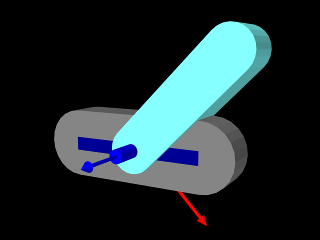
\includegraphics[width=3.1in]{images/SlottedHingeJointDemo}\\
 \else
   \includegraphics[width=1.75in]{images/slottedHingeJoint}&
   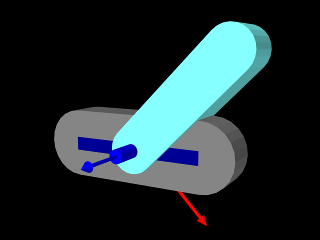
\includegraphics[width=2.333in]{images/SlottedHingeJointDemo}\\
 \fi
\end{tabular}
\end{center}
\caption{Coordinate frames (left) and demo model (right)
for the slotted hinge joint.}
\label{SlottedHingeJoint:fig}
\end{figure}

The \javaclass[artisynth.core.mechmodels]{SlottedHingeJoint} 
(Figure \ref{SlottedHingeJoint:fig}) is
a 2 DOF joint that constrains motion between frames C and D to
translation along the $x$ axis and rotation about the $z$ axis of D.
It implements six constraints and two coordinates $x$ and $\theta$
(Table \ref{SlottedHingeConstraints:tbl}), to which the joint
transform $\T_{CD}$ is related by
%
\begin{equation}
\T_{CD} = \matl
\cos(\theta) & -\sin(\theta) & 0 & x \\
\sin(\theta) &  \cos(\theta) & 0 & 0 \\
0 & 0 & 1 & 0 \\
0 & 0 & 0 & 1 
\matr.
\label{SlottedHingeTCD:eqn}
\end{equation}
%\
The value and ranges for $x$ and $\theta$ are exported by the
properties {\sf x}, {\sf theta}, {\sf xRange} and {\sf thetaRange},
and the coordinate indices are defined by the constants {\tt X\_IDX}
and {\tt THETA\_IDX}. For rendering, the properties {\sf shaftLength}
and {\sf shaftRadius} control the size of a shaft drawn about the
rotation axis, while {\sf slotWidth} and {\sf slotDepth} control the
width and depth of a slot drawn along the sliding ($x$) axis; both are
drawn using the {\sf faceColor} rendering property. When rendering the
slot, its bounds along the $x$ axis are set to {\sf xRange} by
default. However, this may be too large, particularly if {\sf xRange}
is unbounded. As an alternate, the property {\sf slotRange} will be
used instead if its range (i.e., the upper bound minus the lower
bound) exceeds 0.  A demo of {\tt SlottedHingeJoint} is provided by
{\tt artisynth.demos.mech.SlottedHingeJointDemo}.

In addition to the standard constructors described in
Section \ref{CreatingJoints:sec},
% method table
\begin{lstlisting}[]
  SlottedHingeJoint (bodyA, bodyB, originD, zaxis)
\end{lstlisting}
%
creates a slotted hinge joint with a specified origin and $z$ axis direction
for frame D (in world coordinates), and frames C and D coincident.

\begin{table}[h]
\centering
\begin{tabular}{|l|l|l|}
\hline
Index & type/name & description \\
\hline
0 & bilateral & restricts translation along $y$ \\
1 & bilateral & restricts translation along $z$ \\
2 & bilateral & restricts rotation about $x$ \\
3 & bilateral & restricts rotation about $y$ \\
4 & unilataral & enforces limits on the $x$ coordinate \\
5 & unilataral & enforces limits on the $\theta$ coordinate \\
\hline
\hline
0 & $x$ & translation of $C$ along the $x$ axis \\
1 & $\theta$ & rotation of $C$ about the $z$ axis \\
\hline
\end{tabular}
\caption{Constraints (top) and coordinates (bottom) for the slotted hinge joint.}
\label{SlottedHingeConstraints:tbl}
\end{table}

\subsection{Universal joint}

\begin{figure}[h]
\begin{center}
\begin{tabular}{c@{\hskip .5in}c}
 \iflatexml
   \includegraphics[width=2.333in]{images/universalJoint}&
   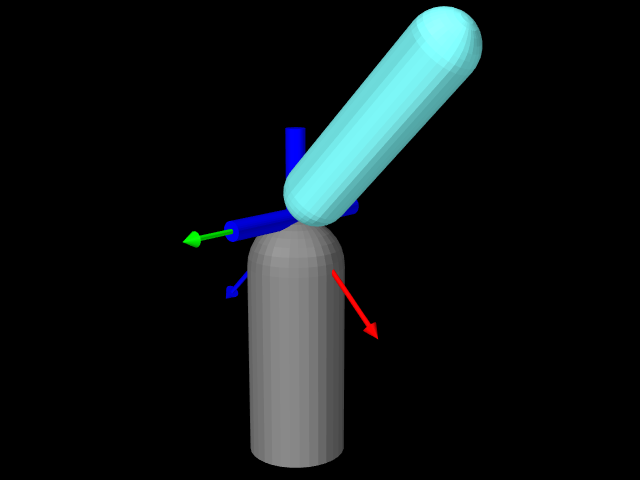
\includegraphics[width=3.1in]{images/UniversalJointDemo}\\
 \else
   \includegraphics[width=1.75in]{images/universalJoint}&
   \includegraphics[width=2.333in]{images/UniversalJointDemo}\\
 \fi
\end{tabular}
\end{center}
\caption{Coordinate frames (left) and demo model (right)
for the universal joint.}
\label{UniversalJoint:fig}
\end{figure}

\begin{table}[h]
\centering
\begin{tabular}{|l|l|l|}
\hline
Index & type/name & description \\
\hline
0 & bilateral & restricts translation along $x$ \\
1 & bilateral & restricts translation along $y$ \\
2 & bilateral & restricts translation along $z$ \\
3 & bilateral & restricts rotation about the final $x$ axis of C \\
4 & unilataral & enforces limits on the roll coordinate \\
5 & unilataral & enforces limits on the pitch coordinate \\
\hline
\hline
0 & $\theta$ (roll) & first rotation of $C$ about the $z$ axis of D \\
1 & $\phi$ (pitch) & second rotation of $C$ about the rotated $y'$ axis \\
\hline
\end{tabular}
\caption{Constraints (top) and coordinates (bottom) for the universal joint.}
\label{UniversalConstraints:tbl}
\end{table}

The \javaclass[artisynth.core.mechmodels]{UniversalJoint} 
(Figure \ref{UniversalJoint:fig}) is a 2 DOF joint
that allows C two rotational degrees of freedom with respect to D: a
{\it roll} rotation $\theta$ about D's $z$ axis, followed by a {\it
pitch} rotation $\phi$ about the rotated $y'$ axis. It implements six
constraints and the two coordinates $\theta$ and $\phi$
(Table \ref{UniversalConstraints:tbl}), to which the joint transform
$\T_{CD}$ is related by
%
\begin{equation*}
\T_{CD} = \matl
\Cr \Cp & -\Sr & \Cr \Sp & 0 \\
\Sr \Cp & \Cr & \Sr \Sp & 0 \\
-\Sp & 0 & \Cp & 0 \\
0 & 0 & 0 & 1 
\matr,
\end{equation*}
%\
where 
%
\begin{equation*}
\Cr \equiv \cos(\theta),\; 
\Sr \equiv \sin(\theta),\;
\Cp \equiv \cos(\phi),\;
\Sp \equiv \sin(\phi).
\end{equation*}
%
The value and ranges for $\theta$ and $\phi$ are exported by the
properties {\sf roll}, {\sf pitch}, {\sf rollRange} and {\sf
pitchRange}, and the coordinate indices are defined by the constants
{\tt ROLL\_IDX} and {\tt PITCH\_IDX}.  

For rendering, the properties {\sf shaftLength} and {\sf shaftRadius} control
the size of shafts drawn about the roll and pitch axes, while {\sf jointRadius}
specifies the radius of a ball drawn around the origin of D; both are drawn
using the {\sf faceColor} rendering property. It is also
possible to add a rendering mesh, using the methods:
% method table
\begin{lstlisting}[]
  void setRenderMesh (PolygonalMesh mesh)
  PolygonalMesh getRenderMesh()
\end{lstlisting}
%
If present, the rendering mesh is rendered in the intermediate
frame between D and C, i.e., D rotated about $z$ by $\theta$.
Rendering is controlled by the face rendering properties (
{\sf faceStyle}, {\sf faceColor}, etc.).

A demo is provided by {\tt artisynth.demos.mech.UniversalJointDemo}.

\subsection{Skewed universal joint}

The \javaclass[artisynth.core.mechmodels]{SkewedUniversalJoint}
(Figure \ref{SkewedUniversalJoint:fig}) is a version of the universal
joint in which the pitch axis is skewed relative to its nominal direction
by an angle $\alpha$. More precisely, let $x'$ and $y'$ be the $x$ and
$y$ axes of C after the initial roll rotation. For a regular universal
joint, the pitch axis is $y'$, whereas for a skewed universal joint it
is $y'$ rotated by $\alpha$ clockwise about $x'$. The joint still has
2 DOF, but the space of allowed rotations is reduced.

\begin{figure}[hhh]
\begin{center}
\begin{tabular}{c@{\hskip .5in}c}
 \iflatexml
   \includegraphics[width=2.333in]{images/skewedUniversalJoint}&
   \includegraphics[width=3.1in]{images/SkewedUniversalJointDemo}\\
 \else
   \includegraphics[width=1.75in]{images/skewedUniversalJoint}&
   \includegraphics[width=2.333in]{images/SkewedUniversalJointDemo}\\
 \fi
\end{tabular}
\end{center}
\caption{Left: diagram for a skewed universal joint, showing the 
pitch axis (dotted line) skewed by an angle $\alpha$ relative to its
nominal direction along the $y'$ axis. Right: demo model with skew
angle of $30^\circ$.}
\label{SkewedUniversalJoint:fig}
\end{figure}

The constraints and the coordinates are the same as for the universal
joint, although the relationship between $\T_{CD}$ is now more complicated.
With $\Cr$, $\Sr$, $\Cp$, and $\Sp$ defined as for the universal
joint, $\T_{CD}$ is given by
%
\begin{equation*}
\T_{CD} = \matl
\Cr\Cp - \Sr\Sa\Sp & -\Sr\beta - \Sa\Cr\Sp & \Ca(\Cr\Sp - \Sa\Sr\Vp) & 0 \\
\Sr\Cp + \Cr\Sa\Sp & \Cr\beta - \Sa\Sr\Sp  & \Ca(\Sr\Sp + \Sa\Cr\Vp) & 0 \\
-\Ca \Sp           & \Ca\Sa\Vp             &  \Sa^2 + \Ca^2\Cp       & 0 \\
0 & 0 & 0 & 1 
\matr,
\end{equation*}
%\
where 
%
\begin{equation*}
\Ca \equiv \cos(\alpha), \quad
\Sa \equiv \sin(\alpha), \quad
\Vp \equiv 1 - \Cp, \quad \beta \equiv \Ca^2 + \Sa^2 \Cp.
\end{equation*}
%
Rendering is controlled using the properties {\sf shaftLength}, {\sf
shaftRadius} and {\sf jointRadius} in the same way as for the {\tt
UniversalJoint}.  A demo is provided by calling {\tt
artisynth.demos.mech.UniversalJointDemo} with the model arguments {\tt
-skew <angDeg>}, where {\tt <angDeg>} is the desired skew angle in
degrees.

Constructors for skewed universal joints take the standard forms
described in Section \ref{CreatingJoints:sec}, with an additional
argument at the end indicating the skew angle:
% method table
\begin{lstlisting}[]
  SkewedUniveralJoint (bodyA, TCA, bodyB, TCB, skewAngle)

  SkewedUniveralJoint (bodyA, bodyB, TDW, skewAngle)

  SkewedUniveralJoint (bodyA, bodyB, TCW, TDW, skewAngle)
\end{lstlisting}
%
In addition, the constructor
% method table
\begin{lstlisting}[]
  SkewedUniveralJoint (bodyA, bodyB, originD, rollAxis, pitchAxis)
\end{lstlisting}
%
creates a skewed universal joint specifying the origin of frame D
together with the directions of the roll and pitch axes (in world
coordinates). Frames C and D are coincident and the skew angle is
inferred from the angle between the axes.

\subsection{Gimbal joint}

\begin{figure}[h]
\begin{center}
\begin{tabular}{c@{\hskip .5in}c}
 \iflatexml
   \includegraphics[width=2.333in]{images/sphericalJoint2}&
   \includegraphics[width=3.1in]{images/GimbalJointDemo}\\
 \else
   \includegraphics[width=1.75in]{images/sphericalJoint2}&
   \includegraphics[width=2.333in]{images/GimbalJointDemo}\\
 \fi
\end{tabular}
\end{center}
\caption{Coordinate frames (left; rotation angles not shown) 
and demo model (right) for the gimbal joint.}
\label{GimbalJoint:fig}
\end{figure}

The \javaclass[artisynth.core.mechmodels]{GimbalJoint}
(Figure \ref{GimbalJoint:fig}) is a 3 DOF spherical joint that anchors
the origins of C and D together but otherwise allows C complete
rotational freedom. The rotational degrees of freedom are
parameterized by three roll-pitch-yaw angles, denoted by
$\theta, \phi, \psi$, which define a rotation $\theta$ about D's $z$
axis, followed by a second rotation $\phi$ about the rotated $y'$
axis, followed by a third rotation $\psi$ about the final $x''$ axis.
It implements six constraints and the three coordinates
$\theta, \phi, \psi$ (Table \ref{GimbalConstraints:tbl}), to which the
joint transform $\T_{CD}$ is related by
%
\begin{equation*}
\T_{CD} = \matl
\Cr \Cp & \Cr \Sp \Sy - \Sr \Cy & \Cr \Sp \Cy + \Sr \Sy & 0 \\
\Sr \Cp & \Sr \Sp \Sy + \Cr \Cy & \Sr \Sp \Cy - \Cr \Sy & 0 \\
-\Sp & \Cp \Sy & \Cp \Cy & 0 \\
0 & 0 & 0 & 1 
\matr,
\end{equation*}
%\
where 
%
\begin{equation*}
\Cr \equiv \cos(\theta),\;
\Sr \equiv \sin(\theta),\;
\Cp \equiv \cos(\phi),\;
\Sp \equiv \sin(\phi),\;
\Cy \equiv \cos(\psi),\;
\Sy \equiv \sin(\psi).
\end{equation*}
%
The value and ranges for $\theta, \phi, \psi$ are exported by the
properties {\sf roll}, {\sf pitch}, {\sf yaw}, {\sf rollRange}, {\sf
pitchRange}, and {\sf yawRange}, and the coordinate indices are
defined by the constants {\tt ROLL\_IDX}, {\tt PITCH\_IDX}, and {\tt
YAW\_IDX}. For rendering, the property {\sf jointRadius} specifies the
radius of a ball drawn around the origin of D, using the {\sf
faceColor} rendering property.  A demo is provided by {\tt
artisynth.demos.mech.GimbalJointDemo}.

In addition to the standard constructors described in
Section \ref{CreatingJoints:sec},
% method table
\begin{lstlisting}[]
  GimbalJoint (bodyA, bodyB, originD)
\end{lstlisting}
%
creates a gimbal joint with a specified origin for frame D (in world
coordinates), and frames C and D coincident and world aligned.

\begin{sideblock}
The constraints implementing {\tt GimbalJoint} are designed so that it
is immune to {\it gimbal lock}, in which a degree of freedom is lost
when $\phi = \pm \pi/2$. However, the coordinate values themselves are
not immune to this singularity, and neither are the unilateral
constraints which enforce limits on their values. Therefore, if
coordinate limits are implemented, the joint should be deployed so as try
and avoid pitch values near $\pm \pi/2$.
\end{sideblock}

\begin{table}[h]
\centering
\begin{tabular}{|l|l|l|}
\hline
Index & type/name & description \\
\hline
0 & bilateral & restricts translation along $x$ \\
1 & bilateral & restricts translation along $y$ \\
2 & bilateral & restricts translation along $z$ \\
3 & unilataral & enforces limits on the roll coordinate \\
4 & unilataral & enforces limits on the pitch coordinate \\
5 & unilataral & enforces limits on the yaw coordinate \\
\hline
\hline
0 & $\theta$ (roll) & first rotation of $C$ about the $z$ axis of D \\
1 & $\phi$ (pitch) & second rotation of $C$ about the rotated $y'$ axis \\
2 & $\psi$ (yaw) & third rotation of $C$ about the final $x''$ axis \\
\hline
\end{tabular}
\caption{Constraints (top) and coordinates (bottom) for the gimbal joint.}
\label{GimbalConstraints:tbl}
\end{table}

\subsection{Spherical joint}

\begin{figure}[h]
\begin{center}
\begin{tabular}{c@{\hskip .5in}c}
 \iflatexml
   \includegraphics[width=2.333in]{images/sphericalJoint3}&
   \includegraphics[width=3.1in]{images/SphericalJointDemo}\\
 \else
   \includegraphics[width=1.75in]{images/sphericalJoint3}&
   \includegraphics[width=2.333in]{images/SphericalJointDemo}\\
 \fi
\end{tabular}
\end{center}
\caption{Left: coordinate frames of the spherical joint, showing the
tilt angle $\phi$ between the $z$ axes of C and D.  Right: demo model
for the spherical joint.}
\label{SphericalJoint:fig}
\end{figure}

The \javaclass[artisynth.core.mechmodels]{SphericalJoint} (Figure
\ref{SphericalJoint:fig}) is a 3 DOF spherical joint that, like
\javaclass[artisynth.core.mechmodels]{GimbalJoint}, anchors the
origins of C and D together but otherwise allows C complete rotational
freedom. {\tt SphericalJoint} does not implement any coordinates, and
so is conceptually more like a {\it ball} joint.  However, it does
provide two choices for limiting its rotation:

\begin{itemize}

\item A limit on the {\it tilt} angle $\phi$ between
the $z$ axes of D and C, such that
%
\begin{equation}
\phi \le \phi_\text{max}.
\end{equation}
%
This is intended to emulate the limit imposed by a ball joint socket.

\item A limit on the total rotation, defined as follows: Let $(\u, \theta)$
be the axis-angle representation of the rotation matrix of $\T_{CD}$,
normalized such that $\theta \ge 0$ and $\|u\| = 1$, and let
$\r_\text{max}$ be a three-vector giving maximum rotation angles with
$x$, $y$, and $z$ components. Then $\theta$ is constrained by
%
\begin{equation}
\theta \le \| \r_\text{max} \circ \u \|,
\end{equation}
%
where $\circ$ denotes the element-wise product. If the components of
$\r_\text{max}$ are set to a uniform value $\theta_\text{max}$, this
simplifies to $\theta \le \theta_\text{max}$.

\end{itemize}

These limits can be enabled by setting the joint's properties {\sf
isTiltLimited} and {\sf isRotationLimited}, respectively, where
enabling one disables the other. The limit values $\phi_\text{max}$
and $\r_\text{max}$ are managed using the properties {\sf maxTilt} and
{\sf maxRotation}, and setting either automatically enables tilt or
rotation limiting, as appropriate. Finally, the tilt angle $\phi$ can
be queried using the (read-only) {\sf tilt} property.  For rendering,
the property {\sf jointRadius} specifies the radius of a ball drawn
around the origin of D, using the {\sf faceColor} rendering
property. A demo of the {\tt SphericalJoint} is provided by {\tt
artisynth.demos.mech.SphericalJointDemo}.

In addition to the standard constructors described in
Section \ref{CreatingJoints:sec},
% method table
\begin{lstlisting}[]
  SphericalJoint (bodyA, bodyB, originD)
\end{lstlisting}
%
creates a spherical joint with a specified origin for frame D (in
world coordinates), and frames C and D coincident and world aligned.

\begin{sideblock}
One should use the rotation limit with some caution, as the
orientations which it prohibits can be somewhat hard to predict,
particularly when $\r_\text{max}$ has non-uniform values.
\end{sideblock}

\begin{table}[h]
\centering
\begin{tabular}{|l|l|l|}
\hline
Index & type/name & description \\
\hline
0 & bilateral & restricts translation along $x$ \\
1 & bilateral & restricts translation along $y$ \\
2 & bilateral & restricts translation along $z$ \\
3 & unilataral & enforces either the ``tilt'' or ``rotation'' limits\\
\hline
\end{tabular}
\caption{Constraints for the spherical joint.}
\label{SphericalConstraints:tbl}
\end{table}

\subsection{Planar joint}

\begin{figure}[h]
\begin{center}
\begin{tabular}{c@{\hskip .5in}c}
 \iflatexml
   \includegraphics[width=2.333in]{images/planarJoint}&
   \includegraphics[width=3.1in]{images/PlanarJointDemo}\\
 \else
   \includegraphics[width=1.75in]{images/planarJoint}&
   \includegraphics[width=2.333in]{images/PlanarJointDemo}\\
 \fi
\end{tabular}
\end{center}
\caption{Coordinate frames (left) and demo model (right)
for the planar joint.}
\label{PlanarJoint:fig}
\end{figure}

The \javaclass[artisynth.core.mechmodels]{PlanarJoint} 
(Figure \ref{PlanarJoint:fig}) is a 3 DOF
joint that constrains C to translation in the $x$-$y$ plane 
and rotation about the $z$ axis of D.  It implements six
constraints and three coordinates $x$, $y$ and $\theta$
(Table \ref{PlanarConstraints:tbl}), to which the joint transform
$\T_{CD}$ is related by
%
\begin{equation*}
\T_{CD} = \matl
\cos(\theta) & -\sin(\theta) & 0 & x \\
\sin(\theta) &  \cos(\theta) & 0 & y \\
0 & 0 & 1 & 0 \\
0 & 0 & 0 & 1 
\matr.
\end{equation*}
%\
The value and ranges for $x$, $y$ and $\theta$ are exported by the
properties {\sf x}, {\sf y}, {\sf theta}, {\sf xRange}, {\sf yRange}
and {\sf thetaRange}, and the coordinate indices are defined by the
constants {\tt X\_IDX}, {\tt Y\_IDX} and {\tt THETA\_IDX}.  
A planar joint can be rendered as a square centered on the origin
of D, using face rendering properties and with a size given by the
{\sf planeSize} property. For example,
%
\begin{lstlisting}[]
  PlanarJoint joint;
  ...
  joint.setPlaneSize (5.0);
  RenderProps.setFaceColor (joint, Color.LIGHT_GRAY);
\end{lstlisting}
%
will cause {\tt joint} to be drawn as a light gray square with size
5.0. The default value of {\sf planeSize} is 0, so drawing the plane
is disabled by default. Also, the default {\sf faceStyle} rendering
property for {\tt PlanarConnector} is set to {\tt FRONT\_AND\_BACK},
so that the plane (when drawn) can be seen from both sides.  A shaft
about the rotation axis can also be drawn, as controlled by the
properties {\sf shaftLength} and {\sf shaftRadius} and using the {\sf
faceColor} rendering property.  A demo is provided by {\tt
artisynth.demos.mech.PlanarJointDemo}.

In addition to the standard constructors described in
Section \ref{CreatingJoints:sec},
% method table
\begin{lstlisting}[]
  PlanarJoint (bodyA, bodyB, originD, zaxis)
\end{lstlisting}
%
creates a planar joint with a specified origin and $z$ axis direction
for frame D (in world coordinates), and frames C and D coincident.

\begin{table}[h]
\centering
\begin{tabular}{|l|l|l|}
\hline
Index & type/name & description \\
\hline
0 & bilateral & restricts translation along $z$ \\
1 & bilateral & restricts rotation about $x$ \\
2 & bilateral & restricts rotation about $y$ \\
3 & unilataral & enforces limits on the $x$ coordinate \\
3 & unilataral & enforces limits on the $y$ coordinate \\
5 & unilataral & enforces limits on the $\theta$ coordinate \\
\hline
\hline
0 & $x$ & translation of $C$ along the $x$ axis of D \\
1 & $y$ & translation of $C$ along the $y$ axis of D \\
2 & $\theta$ & rotation of $C$ about the $z$ axis of D\\
\hline
\end{tabular}
\caption{Constraints (top) and coordinates (bottom) for the planar joint.}
\label{PlanarConstraints:tbl}
\end{table}

\subsection{Planar translation joint}

\begin{figure}[h]
\begin{center}
\begin{tabular}{c@{\hskip .5in}c}
 \iflatexml
   \includegraphics[width=2.333in]{images/planarTranslationJoint}&
   \includegraphics[width=3.1in]{images/PlanarTranslationJointDemo}\\
 \else
   \includegraphics[width=1.75in]{images/planarTranslationJoint}&
   \includegraphics[width=2.333in]{images/PlanarTranslationJointDemo}\\
 \fi
\end{tabular}
\end{center}
\caption{Coordinate frames (left) and demo model (right)
for the planar translation joint.}
\label{PlanarTranslationJoint:fig}
\end{figure}

\begin{table}[h]
\centering
\begin{tabular}{|l|l|l|}
\hline
Index & type/name & description \\
\hline
0 & bilateral & restricts translation along $z$ \\
1 & bilateral & restricts rotation about $x$ \\
2 & bilateral & restricts rotation about $y$ \\
3 & bilateral & restricts rotation about $z$ \\
4 & unilataral & enforces limits on the $x$ coordinate \\
5 & unilataral & enforces limits on the $y$ coordinate \\
\hline
\hline
0 & $x$ & translation of $C$ along the $x$ axis of D \\
1 & $y$ & translation of $C$ along the $y$ axis of D \\
\hline
\end{tabular}
\caption{Constraints (top) and coordinates (bottom) for the planar
translation joint.}
\label{PlanarTranslationConstraints:tbl}
\end{table}

The \javaclass[artisynth.core.mechmodels]{PlanarTranslationJoint} 
(Figure \ref{PlanarTranslationJoint:fig}) is a 2 DOF joint
that is the same as the planar joint without rotation:
C is restricted to translation in the $x$-$y$ plane of D.
It implements six
constraints and two coordinates $x$ and $y$
(Table \ref{PlanarTranslationConstraints:tbl}), to which the joint transform
$\T_{CD}$ is related by
%
\begin{equation*}
\T_{CD} = \matl
1 & 0 & 0 & x \\
0 & 1 & 0 & y \\
0 & 0 & 1 & 0 \\
0 & 0 & 0 & 1 
\matr.
\end{equation*}
%\
The value and ranges for $x$ and $y$ are exported by the properties
{\sf x}, {\sf y}, {\sf xRange} and {\sf yRange}, and the coordinate
indices are defined by the constants {\tt X\_IDX} and {\tt Y\_IDX}.  A
planar translation joint can be rendered as a square centered on the
origin of D, using face rendering properties and with a size given by
the {\sf planeSize} property, in the same way as described for {\tt
PlanarJoint}.  A demo is provided by {\tt
artisynth.demos.mech.PlanarJointDemo}.

In addition to the standard constructors described in
Section \ref{CreatingJoints:sec},
% method table
\begin{lstlisting}[]
  PlanarTranslationJoint (bodyA, bodyB, originD, zaxis)
\end{lstlisting}
%
creates a planar translation joint with a specified origin and $z$
axis direction for frame D (in world coordinates), and frames C and D
coincident.

\subsection{Ellipsoid joint}

The \javaclass[artisynth.core.mechmodels]{EllipsoidJoint} is a 4 DOF
joint that provides similar functionality to the ellipsoidal and
scapulothoracic joints available in OpenSim. It allows the origin of C
to slide around on the surface of an ellipsoid centered on the origin
of D, together with two additional rotational degrees of freedom.

\begin{figure}[h]
\begin{center}
\begin{tabular}{c@{\hskip .5in}c@{\hskip .5in}c}
 \iflatexml
   \includegraphics[width=2.333in]{images/ellipsoidJointS}&
   \includegraphics[width=1.8in]{images/ellipsoidJointC}&
   \includegraphics[width=2.333in]{images/EllipsoidJointDemo}
 \else
   \includegraphics[width=1.75in]{images/ellipsoidJointS}&
   \includegraphics[width=1.4in]{images/ellipsoidJointC}&
   \includegraphics[width=1.75in]{images/EllipsoidJointDemo}
 \fi
\end{tabular}
\end{center}
\caption{Ellipsoidal joint. Left: frame relationships between
D and S (blue). Middle: frame relationships between S and C (blue).
Right: the demo model {\tt EllipsoidJointDemo}, with
$\psi$, $\gamma$, $\theta$ and $\phi$ set to $45^\circ$, $30^\circ$,
$-40^\circ$, and $20^\circ$.}
\label{EllipsoidalJoint:fig}
\end{figure}

The joint kinematics is easiest to describe in terms of an
intermediate frame S whose origin lies on the ellipsoid surface,
with its position controlled by two coordinates: a {\it longitude}
angle $\psi$, and a {\it latitude} angle $\gamma$ (Figure
\ref{EllipsoidalJoint:fig}, left). Frame C has the same origin as
S, with two additional coordinates, $\theta$ and $\phi$ which allow it
to rotate about S (Figure \ref{EllipsoidalJoint:fig}, middle).  If the
transform $\T_{SD}$ from S to D and the (rotational-only) transform
$\T_{CS}$ from C to S are given by
%
\begin{equation*}
\T_{SD} = \matl \R_{SD} & \p_{SD} \\ 0 & 1 \matr
\quad \text{and} \quad
\T_{CS} = \matl \R_{CS} & 0 \\ 0 & 1 \matr,
\end{equation*}
%
then $\T_{CD}$ is given by
%
\begin{equation*}
\T_{CD} = \T_{SD} \T_{CS} =
\matl \R_{SD} \R_{CS} & \p_{SD} \\ 0 & 1 \matr.
\end{equation*}
%
The six constraints and four coordinates of the ellipsoidal joint are
described in table \ref{EllipsoidalConstraints:tbl}.

\begin{table}[h]
\centering
\begin{tabular}{|l|l|l|}
\hline
Index & type/name & description \\
\hline
0 & bilateral & restricts C to the ellipsoid surface and limits rotation \\
1 & bilateral & restricts C to the ellipsoid surface and limits rotation \\
2 & unilateral & enforces limits on the $\psi$ coordinate \\
3 & unilateral & enforces limits on the $\gamma$ coordinate \\
4 & unilataral & enforces limits on the $\theta$ coordinate \\
5 & unilataral & enforces limits on the $\phi$ coordinate \\
\hline
\hline
0 & $\psi$ & longitude angle for origin of S (and C) on the ellipsoid \\
1 & $\gamma$ & latitude angle for origin of S (and C) on the ellipsoid \\
2 & $\theta$ & first rotation of C about the $z$ axis of S \\
3 & $\phi$ & second rotation of C about rotated $x$ (or $x'$ if $\alpha \ne 0$) \\
\hline
\end{tabular}
\caption{Constraints (top) and coordinates (bottom) for the
ellipsoidal joint.}
\label{EllipsoidalConstraints:tbl}
\end{table}

For frame S, if $A$, $B$ and $C$ are the ellipsoid semi-axis lengths
for the $x$, $y$, and $z$ axes, and $c_\psi$, $s_\psi$, $c_\gamma$,
and $s_\gamma$ are the cosines and sines of $\psi$ and $\gamma$, we
can show that
%
\begin{equation*}
\p_{SD} = \matl A \, s_\gamma \\ -B \, s_\psi c_\gamma \\ C \, c_\psi c_\gamma \matr.
\end{equation*}
%
For the orientation of S, the $z$ axis of S is parallel to the surface
normal and the $x$ axis is parallel to the tangent direction imparted
by the latitudinal velocity $\dot\gamma$.  That means $x$ and $z$
axes are parallel to the direction vectors $\d_x$ and $\d_z$
given by
%
\begin{equation}
\d_x = \matl A \, c_\gamma \\ B \, s_\psi s_\gamma \\ -C \, c_\psi s_\gamma \matr
\quad \text{and} \quad
\d_z = \matl p_x/A^2 \\ p_y/B^2 \\ p_z/C^2 \matr.
\label{xzdirections:eqn}
\end{equation}
%
The columns of $\R_{SD}$ are then given by the normalized values
of $\d_x$, $\d_z \times \d_x$, and $\d_z$, respectively.

The rotation $\R_{CS}$ is formed by a rotation $\theta$ about the $z$
axis, followed by a rotation of $\phi$ about the new $x$ axis.
Letting $\Ct$, $\St$, $\Cp$, and $\Sp$ be the cosines and sines of
$\theta$ and $\phi$, we then have
%
\begin{equation*}
\R_{CS} = \matl 
\Ct & -\St \Cp & \St \Sp \\
\St & \Ct \Cp & -\Ct \Sp \\
0 & \Sp & \Cp
\matr.
\end{equation*}
%

If desired, the $\phi$ rotation can instead be performed about a
modified axis $x'$ that makes an angle $\alpha$ with respect to $x$
in the $x$-$y$ plane. $\alpha$ is controlled by the joint's {\sf alpha}
property (default value $0$) and corresponds to the ``winging'' angle
of the OpenSim scapulothoracic joint. If $\alpha \ne 0$,
$\R_{CS}$ takes the more complex form
%
\begin{equation*}
\R_{CS} = \matl 
c_0 \Ca + s_0 \Cp \Sa & c_0 \Sa - s_0 \Cp \Ca & s_0 \Sp \\
s_0 \Ca - c_0 \Cp \Sa & s_0 \Sa + c_0 \Cp \Ca & -c_0 \Sp\\
-\Sp \Sa & \Sp \Ca & \Cp 
\matr
\end{equation*}
%
where $c_0$, $s_0$, $\Ca$, and $\Sa$ are the cosines and sines of
$\theta + \alpha$ and $\alpha$, respectively.

Within an {\tt EllipsoidJoint}, the values and ranges for $\psi$,
$\gamma$, $\theta$ and $\phi$ are exported by the properties {\sf
longitude}, {\sf latitude}, {\sf theta}, {\sf phi}, {\sf
longitudeRange}, {\sf latitudeRange}, {\sf thetaRange}, and {\sf
phiRange}, and the coordinate indices are defined by the constants
{\tt LONGITUDE\_IDX}, {\tt LATITUDE\_IDX}, {\tt THETA\_IDX}, and {\tt
PHI\_IDX}.  For rendering, the property {\sf drawEllipsoid} specifies
whether the ellipsoid surface should be drawn; if {\tt true}, it will
be drawn using the joint's face rendering properties.  A demo is
provided by {\tt artisynth.demos.mech.EllipsoidJointDemo}.

Ellipsoid joints can be created with the following constructors:
%
\begin{lstlisting}[]
  EllipsoidJoint (A, B, C, alpha, openSimCompatible)

  EllipsoidJoint (rbodyA, TCA, rbodyB, TDB, A, B, C, alpha, openSimCompatible)

  EllipsoidJoint (cbodyA, cbodyB, TCW, TDW, A, B, C)
\end{lstlisting}
%
The first of these creates a joint that is {\it not} attached to any
bodies; attachment can be done later using one of the {\tt
setBodies()} methods.  Its semi-axis lengths are given by {\tt A},
{\tt B}, and {\tt C}, its $\alpha$ angle is given by {\tt alpha}, and
the argument {\tt openSimCompatible}, if {\tt true}, makes the joint
kinematics compatible with OpenSim (Section \ref{OpenSimCompat:sec}).
The second constructor creates a joint and then attaches it to rigid
bodies {\tt rbodyA} and {\tt rbodyB}, with the specified $\T_{CA}$ and
$\T_{DB}$ transformations. The third constructor creates a joint and
attaches it to connectable bodies {\tt cbodyA} and {\tt cbodyB}, with
the locations of the C and D frames specified in world coordinates by
{\tt TCW} and {\tt TDW}.

\begin{sideblock}
Unlike in many joints, $\T_{CD}$ is {\it not} the identity when the
joint coordinates are all $0$. That is because the origin of C must
lie on the ellipsoid surface, and since D is at the center of the
ellipsoid, $\T_{CD}$ can never be the identity. In particular,
when all coordinate values are 0, $\R_{CD} = \I$ but
$\p_{CD} = \p_{SD} = (0, 0, C)^T$.
\end{sideblock}

\subsubsection{OpenSim compatibility}
\label{OpenSimCompat:sec}

The {\tt openSimCompatible} argument in some of the joint's
constructors makes the kinematics compatible with the ellipsoidal
joint used by OpenSim. This means that $\R_{SD}$ is computed
differently: in OpenSim, instead of
using (\ref{xzdirections:eqn}), the $z$ and $x$ axis directions of
$\R_{SD}$ are computed using
%
\begin{equation}
\d_x = \matl c_\gamma \\ s_\psi s_\gamma \\ -c_\psi s_\gamma \matr
\quad \text{and} \quad
\d_z = \matl p_x/A \\ p_y/B \\ p_z/C \matr.
\end{equation}
%
In particular, this means that the $z$ axis is only approximately
parallel to the ellipsoid surface normal.

\begin{sideblock}
In OpenSim, the axes of the C frame of both the ellipsoid and
scapulothoracic joints are oriented differently that those of the
ArtiSynth joint: they are rotated by $-\pi/2$ about $z$, so that the
$x$ and $y$ axes correspond to the $-y$ and $x$ axes of the ArtiSynth
joint.
\end{sideblock}

\subsection{Solid joint}

The \javaclass[artisynth.core.mechmodels]{SolidJoint} 
is a 0 DOF joint that rigidly constrains C to D.  It
implements six constraints and no coordinates
(Table \ref{SolidJointConstraints:tbl}) and the resulting $\T_{CD}$ is the
identity.

\begin{sideblock}
There aren't normally many uses for solid joints. If one wishes to
create a complex rigid body by joining together a variety of shapes,
this can be done more efficiently by making these shapes mesh
components of a single rigid body
(Section \ref{rigidBodyMultipleMeshes:sec}).
\end{sideblock}

\begin{table}[h]
\centering
\begin{tabular}{|l|l|l|}
\hline
Index & type/name & description \\
\hline
0 & bilateral & restricts translation along $x$ \\
1 & bilateral & restricts translation along $y$ \\
2 & bilateral & restricts translation along $z$ \\
3 & bilateral & restricts rotation about $x$ \\
4 & bilateral & restricts rotation about $y$ \\
5 & bilateral & restricts rotation about $z$ \\
\hline
\end{tabular}
\caption{Constraints for the solid joint.}
\label{SolidJointConstraints:tbl}
\end{table}

\subsection{Planar Connector}

\begin{figure}[h]
\begin{center}
\begin{tabular}{c}
 \iflatexml
   \includegraphics[]{images/PlanarConnectorDemo}\\
 \else
   \includegraphics[width=3.00in]{images/PlanarConnectorDemo}\\
 \fi
\end{tabular}
\end{center}
\caption{Demo model for the planar connector, in which
a corner point of a box is constrained to the $x$-$y$ plane of D.}
\label{PlanarConnector:fig}
\end{figure}

\begin{table}[h]
\centering
\begin{tabular}{|l|l|l|}
\hline
Index & type/name & description \\
\hline
0 & bilateral {\it or} unilateral & restricts translation along $z$ \\
\hline
\end{tabular}
\caption{Constraints for the planar connector.}
\label{PlanarConnectorConstraints:tbl}
\end{table}

The \javaclass[artisynth.core.mechmodels]{PlanarConnector}
(Figure \ref{PlanarConnector:fig}) is a 5 DOF connector that attaches
the origin of C to the $x$-$y$ plane of D. C is completely free to
rotate, and to translate within the $x$-$y$ plane. Only motion in the
$z$ direction is restricted. {\tt PlanarConnector} implements one
constraint and has no coordinates
(Table \ref{PlanarConnectorConstraints:tbl}).

A {\tt PlanarConnector} constrains a point on body A (located at the
origin of C) to move within a plane on body B. Several planar
connectors can be employed to constrain body motions in more
complicated ways, although one must be careful to avoid
overconstraining the system. The connector can also be configured to
function {\it unilaterally}, via its {\sf unilateral} property, in
which case the point is constrained to lie in the half-space defined by
$z \ge 0$ with respect to D. Several unilateral {\tt PlanarConnector}s
can therefore be used to implement a cheap and approximate collision
mechanism with fixed collision points.

\begin{sideblock}
When set to function unilaterally, overconstraining the system is not
an issue because of the way in which ArtiSynth solves unilateral
constraints.
\end{sideblock}

A planar connector can be rendered as a square centered on the origin
of D, using face rendering properties and with a size given by the
{\sf planeSize} property. The point attached to A can also be rendered
using point rendering properties. For example,
%
\begin{lstlisting}[]
  PlanarConnector connector;
  ...
  connector.setPlaneSize (5.0);
  RenderProps.setFaceColor (connector, Color.LIGHT_GRAY);
  RenderProps.setSphericalPoints (connector, 0.1, Color.BLUE);
\end{lstlisting}
%
will cause {\tt connector} to be drawn as a light gray square with
size 5, and for the point on body A to be drawn as a blue sphere with
radius 0.1. The default value of {\sf planeSize} is 0, so drawing the
plane is disabled by default. Also, the default {\sf faceStyle}
rendering property for {\tt PlanarConnector} is set to {\tt
FRONT\_AND\_BACK}, so that the plane (when drawn) can be seen from
both sides.

Constructors for the {\tt PlanarConnector} include
% method table
\begin{lstlisting}[]
  PlanarConnector (bodyA, pCA, bodyB, TDB)

  PlanarConnector (bodyA, pCA, TDW)

  PlanarConnector (bodyA, bodyA, TDW)
\end{lstlisting}
%
where {\tt pCA} gives the connection point of body A {\it with respect
to frame A}, {\tt TDB} gives the transform from frame D
to frame B, and {\tt TDW} gives the transform from frame D to world.

\subsection{Segmented Planar Connector}

\begin{figure}[h]
\begin{center}
\begin{tabular}{c@{\hskip .5in}c}
 \iflatexml
   \includegraphics[width=2.333in]{images/segmentedPlanarConnector}&
   \includegraphics[width=3.1in]{images/SegmentedPlaneDemo}\\
 \else
   \includegraphics[width=1.75in]{images/segmentedPlanarConnector}&
   \includegraphics[width=2.333in]{images/SegmentedPlaneDemo}\\
 \fi
\end{tabular}
\end{center}
\caption{Left: cross-section in the $x$-$z$ plane of frame $D$ showing
the segments of a segmented planar connector, with the points defining
the segments shown as black dots.  Right: demo model for the segmented
planar connector.}
\label{SegmentedPlanarConnector:fig}
\end{figure}

\begin{table}[h]
\centering
\begin{tabular}{|l|l|l|}
\hline
Index & type/name & description \\
\hline
0 & bilateral {\it or} unilateral & restricts translation normal to the surface \\
\hline
\end{tabular}
\caption{Constraints for the segmented planar connector.}
\label{SegmentedPlanarConstraints:tbl}
\end{table}

The \javaclass[artisynth.core.mechmodels]{SegmentedPlanarConnector}
(Figure \ref{SegmentedPlanarConnector:fig}) is a 5 DOF connector that
generalizes {\tt PlanarConnector} to a piecewise linear surface, to
which the origin of $C$ is constrained while $C$ is otherwise
completely free to rotate. The surface is specified by a sequence of
2D points defining a piecewise linear curve in the $x$-$z$ plane of D
(Figure \ref{SegmentedPlanarConnector:fig}, left). This curve does not
need to be a function; the segment nearest to C is the one used to
enforce the constraint at any given time. The surface has infinite
extent and is extrapolated beyond the first and last segments.  It
implements one constraint and has no coordinates (Table
\ref{SegmentedPlanarConstraints:tbl}).

By appropriate choice of segments, a {\tt SegmentedPlanarConnector}
can approximate any surface defined by a curve in the $x$-$z$ plane.
As with {\tt PlanarConnector}, it can also be configured as
unilateral, constraining the origin of $C$ to lie on the side of the
surface defined by the normal vectors $\n_k$ of each segment $k$. If
$\p_{k-1}$ and $\p_k$ are the points in the $x$-$z$ plane defining the
$k$-th segment, and $\hat\y$ is the $y$ axis unit vector, then $\n_k$
is given by
%
\begin{equation}
\n_k = \frac{\u \times \hat\y}{\| \u \times \hat\y\|},
\quad \u \equiv \p_{k} -\p_{k-1}.
\end{equation}
%

The properties controlling the rendering of a segmented planar
connector are the same as for a planar connector, with each of the
individual plane segments drawn as a rectangle whose length along the
$y$ axis is controlled by {\sf planeSize}.

Constructors for a {\tt SegmentedPlanarConnector} are analogous to
those used for {\tt PlanarConnector},
% method table
\begin{lstlisting}[]
  SegmentedPlanarConnector (bodyA, pCA, bodyB, TDB, segs)

  SegmentedPlanarConnector (bodyA, pCA, TDW, segs)

  SegmentedPlanarConnector (bodyA, bodyA, TDW, segs)
\end{lstlisting}
%
where {\tt segs} is an additional argument of type {\tt double[]}
giving the 2D coordinates defining the segments in the $x$-$z$ plane.

\subsection{Legacy Joints}

ArtiSynth maintains three legacy joint for compatibility with earlier
software:

\begin{itemize}

\item \javaclass[artisynth.core.mechmodels]{RevoluteJoint} is identical
to the \javaclass[artisynth.core.mechmodels]{HingeJoint}, except that
its coordinate $\theta$ is oriented {\it clockwise} about the $z$ axis
instead of {\it counter-clockwise}. Rendering is also done
differently, with shafts about the rotation axis drawn using
line rendering properties.

\item \javaclass[artisynth.core.mechmodels]{RollPitchJoint} is identical
to the \javaclass[artisynth.core.mechmodels]{UniversalJoint}, except
that its roll-pitch coordinates $\theta, \phi$ are computed with
respect to the rotation $\R_{DC}$ from frame D to C, instead of the
rotation $\R_{CD}$ from frame C to D. Rendering is also done
differently, with shafts along the roll and pitch axes drawn
using line rendering properties, and the ball around the
origin of D drawn using point rendering properties.

\item \javaclass[artisynth.core.mechmodels]{SphericalRpyJoint}
is identical to
the \javaclass[artisynth.core.mechmodels]{GimbalJoint}, except that
its roll-pitch-yaw coordinates $\theta, \phi, \psi$ are computed with
respect to the rotation $\R_{DC}$ from frame D to C, instead of the
rotation $\R_{CD}$ from frame C to D. Rendering is also done
differently, with the ball around the origin of D drawn using point
rendering properties.

\end{itemize}

\subsection{Example: A multijointed arm}

\label{MultiJointedArm:sec}

\begin{figure}[ht]
\begin{center}
\begin{tabular}{cc}
 \iflatexml \includegraphics[]{images/MultiJointedArmInit}& \includegraphics[]{images/MultiJointedArm}\\ \else \includegraphics[height=2.5in]{images/MultiJointedArmInit}& \includegraphics[height=2.5in]{images/MultiJointedArm}\\ \fi
\end{tabular}
\end{center}
\caption{{\tt MultiJointedArm} as initially assembled in code (left),
and after repositioning by moving the joint angles (right).}
\label{MultiJointedArm:fig}
\end{figure}

The example model
%
\begin{verbatim}
  artisynth.demos.tutorial.MultiJointedArm
\end{verbatim}
%
shows two links connected by universal and hinge joints to form a 3 DOF
robot-like arm. The model class definition, excluding the include directives,
is shown here:
%
\lstset{numbers=left}
\iflatexml
%% Hack: latexml lstinputlisting doesn't handle firstline correctly
\lstset{firstnumber={-23}}
\lstinputlisting[firstline=1]{../../src/artisynth/demos/tutorial/MultiJointedArm.java}
\lstset{firstnumber={1}}
\else
\lstinputlisting[firstline=25]{../../src/artisynth/demos/tutorial/MultiJointedArm.java}
\fi
\lstset{numbers=none}
%
Line 3 uses {\tt getSourceRelativePath()} to locate the geometry folder
relative to the model's source folder and lines 4-5 define some constants.  The
{\tt build()} method begins by creating and adding a {\tt MechModel},
specifying a standard inertial damping of 1, as well as a rotary damping value
to reduce spinning of the first joint about the $z$ axis. The class member
variable {\tt myMech} is used to store a reference to the {\tt MechModel} so
that it is available to subclasses.

A {\tt FixedMeshBody} is used to illustrate a mounting plate (lines 15-21);
this is purely decorative and has no dynamic purpose. The links and joints are
then created and assembled in the configuration shown in
Figure \ref{MultiJointedArm:fig} (left). The first link, {\tt link0}, is
created from a rounded-box mesh, and then repositioned to align vertically
along the $z$ axis under the mounting plate (lines 23-31).  The link is then
attached to ground, just below the mounting plate, using a 2 DOF universal
joint (lines 33-42), with a rendering mesh added to illustrate a mounting
bracket and a range limit of $\pm 240^\circ$ set on the roll angle. (Note that
similar physics could be achieved with two hinge joints and an additional
link.) The second link, {\tt link1}, is then also created from a rounded-box
mesh and repositioned vertically along the $z$ axis under {\tt link0} (lines
41-52), to which it is attached using a hinge joint (lines 54-60).

After the linkage has been assembled, some marker points are added to the
links (lines 62-67), and the linkage is repositioned by setting some of the
joint coordinates (lines 70-72) to assume the configuration shown in
Figure \ref{MultiJointedArm:fig} (right). Finally, some
additional render properties are set (lines 73-78).

To run this example in ArtiSynth, select {\sf All demos > tutorial >
MultiJointedArm} from the {\sf Models} menu. The model should load and
initially appear as in Figure \ref{MultiJointedArm:fig}.  Running the model
will cause the links to fall under gravity.  Forces can also be interactively
applied using the pull tool (see the section ``Pull Manipulation'' in the
\artisynthManual{uiguide}{ArtiSynth User Interface Guide}).

\section{Frame springs}
\label{FrameSprings:sec}

Another way to connect two rigid bodies together is to use a {\it
frame spring}, which is a six dimensional spring that generates
restoring forces and moments between coordinate frames.

\subsection{Frame spring coordinate frames}

\begin{figure}[ht]
\begin{center}
 \iflatexml
   \includegraphics[width=3in]{images/frameSpring}
 \else
   \includegraphics[width=3in]{images/frameSpring}
 \fi
\end{center}
\caption{A frame spring connecting two coordinate frames D and C.}
\label{frameSpring:fig}
\end{figure}

The basic idea of a frame spring is shown in Figure
\ref{frameSpring:fig}. It generates restoring forces and moments on
two frames C and D which are a function of $\T_{DC}$ and $\hat\v_{DC}$
(the spatial velocity of frame D with respect to frame C).

Decomposing forces into stiffness and damping terms, the force
$\f_C$ and moment $\Btau_C$ acting on C can be expressed as 
%
\begin{align}
\f_C & = \f_{k} (\T_{DC}) + \f_{d} (\hat\v_{DC}) \notag \\
\Btau_C & = \Btau_{k} (\T_{DC}) + \Btau_{d} (\hat\v_{DC}).
\label{ftauC:eqn}
\end{align}
%
where the translational and rotational forces $\f_{k}$, $\f_{d}$,
$\Btau_{k}$, and $\Btau_{d}$ are general functions of $\T_{DC}$ and
$\hat\v_{DC}$.

The forces acting on D are equal and opposite, so that
%
\begin{align}
\f_D & = - \f_C, \notag \\
\Btau_D & = - \Btau_C.
\label{ftau2:eqn}
\end{align}
%

\begin{figure}[ht]
\begin{center}
 \iflatexml
   \includegraphics[width=3in]{images/frameSpringBodies}
 \else
   \includegraphics[width=3in]{images/frameSpringBodies}
 \fi
\end{center}
\caption{A frame spring connecting two rigid bodies A and B.}
\label{frameSpringBodies:fig}
\end{figure}

If frames C and D are attached to a pair of rigid bodies A and B, then
a frame spring can be used to connect them in a manner analogous to a
joint. As with joints, C and D generally do not coincide with the body
frames, and are instead offset from them by fixed transforms $\T_{CA}$
and $\T_{DB}$ (Figure \ref{frameSpringBodies:fig}).

\begin{sideblock}

For historical reasons, the default behavior for frame springs is to base the
restoring forces on $\T_{DC}$ and $\hat\v_{DC}$, as per (\ref{ftauC:eqn}).
However, it may be more convenient to instead use $\T_{CD}$ and $\hat\v_{CD}$
and compute the force $\f_D$ and moment $\Btau_D$ acting on frame D:
%
\begin{align}
\f_D & = \f_{k} (\T_{CD}) + \f_{d} (\hat\v_{CD}) \notag \\
\Btau_D & = \Btau_{k} (\T_{CD}) + \Btau_{d} (\hat\v_{CD}).
\label{ftauD:eqn}
\end{align}
%
For example, using $\T_{CD}$ is consistent with the usual coordinate frame
conventions for joints, and so may be preferable when a spring is being used as
a ``soft'' replacement for a joint.  To use $\T_{CD}$ instead of $\T_{DC}$, the
application should set the spring's {\sf useTranformDC} property to {\tt false}.
\end{sideblock}

\subsection{Frame materials}

The restoring forces (\ref{ftauC:eqn}) generated in a frame spring
depend on the {\it frame material} associated with the spring. Frame
materials are defined in the package {\tt artisynth.core.materials},
and are subclassed from
\javaclass[artisynth.core.materials]{FrameMaterial}.
The most basic type of material is a 
\javaclass[artisynth.core.materials]{LinearFrameMaterial},
in which the restoring forces are determined from
%
\begin{align*}
\f_C & = 
\K_{t} \, \x_{DC} + \D_{t} \, \v_{DC} \\
\Btau_C & = 
\K_{r} \, \hat\Bthe_{DC} + \D_{r} \, \Bom_{DC}
\label{flinear:eqn}
\end{align*}
%
where $\hat\Bthe_{DC}$ gives the small angle approximation of the
rotational components of $\T_{DC}$ with respect to the $x$, $y$, and
$z$ axes, and
%
\begin{gather*}
\K_{t} \equiv 
\matl k_{tx} & 0 & 0 \\ 0 & k_{ty} & 0 \\ 0 & 0 & k_{tz} \matr, \;
\D_{t} \equiv 
\matl d_{tx} & 0 & 0 \\ 0 & d_{ty} & 0 \\ 0 & 0 & d_{tz} \matr, \;\\
\K_{r} \equiv
\matl k_{r x} & 0 & 0 \\ 0 & k_{r y} & 0 \\ 0 & 0 & k_{r z} \matr, \;
\D_{r} \equiv
\matl d_{r x} & 0 & 0 \\ 0 & d_{r y} & 0 \\ 0 & 0 & d_{r z} \matr.
\end{gather*}
%
are the stiffness and damping matrices. The diagonal values defining
each matrix are stored in the 3-dimensional vectors $\k_t$, $\k_r$,
$\d_t$, and $\d_r$ which are exposed as the {\tt stiffness}, {\tt
rotaryStiffness}, {\tt damping}, and {\tt rotaryDamping} properties of
the material. Each of these specifies stiffness or damping values
along or about a particular axis. Specifying different values for
different axes will result in anisotropic behavior.

Other frame materials offering nonlinear behavior may be defined in
{\tt artisynth.core.materials}.

\subsubsection{PowerFrameMaterial}

An useful alternative to {\tt LinearFrameMaterial} 
is \javaclass[\mats]{PowerFrameMaterial}, which computes restoring forces along
each of the translational and rotational directions according to a power law of
the form
%
\begin{equation}
f = k \, \text{sgn} (x) |x|^n
\label{powerForce:eqn}
\end{equation}
%
where $k$ is a stiffness, $x$ is displacement, and $n$ is an exponent
in the range $n \in \{1,2,3\}$. It is also possible to specify both upper and
lower deadbands, $b_u$ and $b_l$, such that if $x_t$ is the true
displacement, $x$ is computed according to
%
\begin{equation}
x = \begin{cases}
x_t - b_l & x_t < b_l, \\
x_t - b_u & x_t > b_u, \\
0 & \text{otherwise} 
\end{cases}.
\label{powerDeadbands:eqn}
\end{equation}
%
{\tt PowerFrameMaterial} effects the same damping behavior as {\tt
LinearFrameMaterial}.

If rotational deadbands are specified, the rotational displacement may be large
enough that the the small angle approximation used for {\tt
LinearFrameMaterial} no longer applies. Therefore, rotational displacements are
computed as the three x-y-z Tait-Bryan angles of $\R_{DC}$.  The use of
these finite displacement angles introduces a coupling such that if $\Btau$ is
the nominal moment produced by applying (\ref{powerForce:eqn}) and
(\ref{powerDeadbands:eqn}) to each of the
three rotational angles, the actual resulting moment $\Btau_C$ is
%
\begin{equation}
\Btau_C = \matl
1 & 0 & 0 \\
\frac{s_y s_x}{c_y} & c_x & -\frac{s_x}{c_y} \\
-\frac{s_y c_x}{c_y} & s_x & \frac{c_x}{c_y}
\matr
\,
\Btau,
\label{rotForceCoupling:eqn}
\end{equation}
%
where $s_x$, $c_x$, $s_y$, $c_y$ are the sines and cosines of the x and y
rotations. The coupling is associated with the non-commutativity of rotations and
the fact that the x-y-z angles have a singularity when the y rotation
approaches $\pm \pi/2$. This appears as the division by $c_y$ in
(\ref{rotForceCoupling:eqn}), and so care should be taken to avoid such
orientations.

The parameters controlling the behavior of {\tt PowerFrameMaterial} can be set
independently for each of the six translational and rotational displacements,
using the following properties, each of which is described by a three-vector:
%
\begin{center}
\begin{tabular}{|l|l|l|} \hline
 & Property & Description \\
\hline
$\k_t$ & {\sf stiffness} & translational stiffness \\
$\n_t$ & {\sf exponents} & translational exponents \\
$\b_{ut}$ & {\sf upperDeadband} & upper deadband for translations \\
$\b_{lt}$ & {\sf lowerDeadband} & lower deadband for translations \\
$\d_t$ & {\sf damping} & translational damping \\
$\k_r$ & {\sf rotaryStiffness} & rotational stiffness \\
$\n_r$ & {\sf rotaryExponents} & rotational exponents \\
$\b_{ur}$ & {\sf upperRotaryDeadband} & upper deadband for rotations \\
$\b_{lr}$ & {\sf lowerRotaryDeadband} & lower deadband for rotations \\
$\d_r$ & {\sf rotaryDamping} & rotational damping \\
\hline
\end{tabular}
\end{center}
Each of these has a default value of $\mathbf{0}$, except for the exponents,
which have a default value of $(\mathbf{1}$.

\begin{figure}[ht]
\begin{center}
\begin{tabular}{ccc}
   \includegraphics[width=2in]{images/PowerFrame1}&
   \includegraphics[width=2in]{images/PowerFrame2}&
   \includegraphics[width=2in]{images/PowerFrame3}
\end{tabular}
\end{center}
\caption{Example force-displacement curves produced by {\tt PowerFrameMaterial}.
Left: linear behavior with $k=20$, $n=1$, $b_l=-0.5$, and $b_u=0.25$;
middle: quadratic behavior with $k=20$, $n=2$, and $b_l= b_u=0$;
right: cubic behavior with $k=80$, $n=3$, $b_l=0$, and $b_u=0.5$.}
\label{PowerFrameMaterial:fig}
\end{figure}

If used with exponents of 1 and no deadbands, {\tt PowerFrameMaterial} behaves
like {\tt LinearFrameMaterial} with finite rotation displacements.  Otherwise,
Figure \ref{PowerFrameMaterial:fig} illustrates some of the force-displacement
curves that can be produced. Using a power $n > 1$ (rightmost panels) has the
advantage of producing a curve that is differentiable.  However, the forces
grow more slowly for smaller displacements; a cubic force (right panel) almost
behaves as if it has a small deadband, even with $b_l = b_u = 0$.

An important application of {\tt PowerFrameMaterial} is creating one-sided
force behaviors by setting $b_l$ or $b_u$ to sufficiently low or high values.

\subsection{Creating frame springs}
\label{CreatingFrameSprings:sec}

Frame springs are implemented by the class
\javaclass[artisynth.core.mechmodels]{FrameSpring}.  Creating a frame
spring generally involves instantiating this class, and then setting
the material, the bodies A and B, and the transforms $\T_{CA}$ and
$\T_{DB}$.

A typical construction sequence might look like this:
%
\begin{lstlisting}[]
  FrameSpring spring = new FrameSpring ("springA");
  spring.setMaterial (new LinearFrameMaterial (kt, kr, dt, dr));
  spring.setFrames (bodyA, bodyB, TDW);
\end{lstlisting}
%
The material is set using
\javamethod*[artisynth.core.mechmodels.FrameSpring]{setMaterial()}.
The example above uses a {\tt LinearFrameMaterial}, created with a
constructor that sets $\k_t$, $\k_r$, $\d_t$, and $\d_r$ to uniform
Isotropic values specified by {\tt kt}, {\tt kr}, {\tt dt}, and {\tt
dr}. 

The bodies and transforms can be set in the same manner as for joints
(Section \ref{CreatingJoints:sec}), with the
methods\\ \javamethodAlt{artisynth.core.mechmodels.FrameSpring.setFrames(Frame,Frame,RigidTransform3d)}{setFrames(bodyA,bodyB,TDW)}
and
\javamethodAlt{artisynth.core.mechmodels.FrameSpring.setFrames(Frame,RigidTransform3d,Frame,RigidTransform3d)}{setFrames(bodyA,TCA,bodyB,TDB)}
assuming the role of the {\tt setBodies()} methods used for joints.
The former takes D specified in world coordinates and computes
$\T_{CA}$ and $\T_{DB}$ assuming that there is no initial spring
displacement (i.e., that $\T_{DC} = \I$), while the latter allows
$\T_{CA}$ and $\T_{DB}$ to be specified explicitly with $\T_{DC}$
assuming whatever value is implied.

Frame springs and joints are often placed together, using the same
transforms $\T_{CA}$ and $\T_{DB}$, with the spring providing
restoring forces to help keep the joint within prescribed bounds.

As with joints, a frame spring can be connected to only a single body,
by specifying {\tt frameB} as {\tt null}. Frame B is then taken to be
the world coordinate frame W.

\subsection{Example: two bodies connected by a frame spring}
\label{LumbarFrameSpring:sec}

\begin{figure}[ht]
\begin{center}
\iflatexml
 \includegraphics[]{images/LumbarFrameSpring}
\else
 \includegraphics[width=3.75in]{images/LumbarFrameSpring}
\fi
\end{center}
\caption{LumbarFrameSpring model loaded into ArtiSynth.}
\label{LumbarFrameSpring:fig}
\end{figure}

A simple model showing two simplified lumbar vertebrae, modeled as
rigid bodies and connected by a frame spring, is defined in
%
\begin{verbatim}
  artisynth.demos.tutorial.LumbarFrameSpring
\end{verbatim}
%
The definition for the entire model class is shown here:
\lstset{numbers=left}
\lstinputlisting{../../src/artisynth/demos/tutorial/LumbarFrameSpring.java}
\lstset{numbers=none}

For convenience, the code to create and add each vertebrae is wrapped
into the method {\tt addBone()} defined at lines 27-32. This method
takes two arguments: the {\tt MechModel} to which the bone should be
added, and the name of the bone. Surface meshes for the bones are
located in {\tt .obj} files located in the directory {\tt
../mech/geometry} relative to the source directory for the model
itself.
\javamethod*[maspack.util]{PathFinder.getSourceRelativePath(,)}
is used to find a proper path to this directory (see Section
\ref{PathFinder:sec}) given the model class type ({\tt
LumbarFrameSpring.class}), and this is stored in the static string
{\tt geometryDir}. Within {\tt addBone()}, the directory path and the
bone name are used to create a path to the bone mesh itself, which is
in turn used to create a {\tt PolygonalMesh} (line 28). The mesh is
then used in conjunction with a {\tt density} to create a rigid body
which is added to the {\tt MechModel} (lines 29-30) and returned.

The {\tt build()} method begins by creating and adding a {\tt
MechModel}, specifying a low value for gravity, and setting the rigid
body damping properties {\tt frameDamping} and {\tt
rotaryDamping} (lines 37-41). (The damping parameters are needed
here because the frame spring itself is created with no damping.)
Rigid bodies representing the vertebrae {\tt lumbar1} and {\tt
lumbar2} are then created by calling {\tt addBone()} (lines 44-45),
{\tt lumbar1} is translated by setting the origin of its pose to
$(-0.016, 0.039, 0)^T$, and {\tt lumbar2} is set to be fixed by making
it non-dynamic (line 47).

\begin{figure}[ht]
\begin{center}
\iflatexml
 \includegraphics[]{images/LumbarFrameSpringNoflip}
\else
 \includegraphics[width=3.75in]{images/LumbarFrameSpringNoflip}
\fi
\end{center}
\caption{LumbarFrameSpring model as it would appear if not rotated
about the $x$ axis.}
\label{LumbarFrameSpringNoflip:fig}
\end{figure}

At this point in the construction, if the model were to be loaded, it
would appear as in Figure \ref{LumbarFrameSpringNoflip:fig}. To change
the viewpoint to that seen in Figure \ref{LumbarFrameSpring:fig}, we
rotate the entire model about the $x$ axis (line 50).  This is done
using
\javamethodAlt{artisynth.core.mechmodels.MechModel.transformGeometry()}
{transformGeometry(X)}, which transforms the geometry of an entire
model using a rigid or affine transform. This method is
described in more detail in Section \ref{TransformingGeometry:sec}.

The frame spring is created and added at lines 54-59, using the
methods described in Section \ref{CreatingFrameSprings:sec}, with
frame D set to the (initial) pose of {\tt lumbar1}.

Render properties are set starting at line 62. By default, a frame
spring renders as a pair of red, green, blue coordinate axes showing
frames C and D, along with a line connecting them. The line width and
the color of the connecting line are controlled by the line render
properties {\tt lineWidth} and {\tt lineColor}, while the length of
the coordinate axes is controlled by the special frame spring property
{\tt axisLength}.

To run this example in ArtiSynth, select {\sf All demos > tutorial >
LumbarFrameSpring} from the {\sf Models} menu. The model should load
and initially appear as in Figure \ref{LumbarFrameSpring:fig}.
Running the model (Section \ref{LoadingAndRunning:sec}) will cause
{\tt lumbar1} to fall slightly under gravity until the frame spring
arrests the motion. To get a sense of the spring's behavior, one can
interactively apply forces to {\tt lumbar1} using the pull tool
(see the section ``Pull Manipulation'' in the
\artisynthManual{uiguide}{ArtiSynth User Interface Guide}).

\section{Other point-based forces}
\label{OtherPointForces:sec}

All ArtiSynth components which are capable of exerting forces, including the
axial springs of Section \ref{ParticlesAndSprings:sec} and the frame springs of
Section \ref{FrameSprings:sec}, are subclasses of
\javaclass[\mech]{ForceComponent}. Other force effector
types include
\javaclass[\mech]{PointPlaneForce} and
\javaclass[\mech]{PointMeshForce}, described in this section.

\subsection{Forces between points and planes or meshes}

A \javaclass[\mech]{PointPlaneForce} component produces forces between a point
and a plane, based on the point's signed distance $d$ from the plane.
Similarly, a \javaclass[\mech]{PointMeshForce} component produces forces
between one or more points and a closed polygonal mesh, based on the signed
distance $d$ to the mesh. These components thus implement ``soft'' constraint
forces that bind points to either a plane or a mesh. If the component's {\sf
unilateral} property is set to {\tt true}, as described below, forces are
applied only when $d < 0$. This allows the simulation of force-based contact
between points and planes or meshes.

\begin{sideblock}
{\tt PointPlaneForce} and {\tt PointMeshForce} can be used for particles, FEM
nodes and point-based markers, all of which are subclasses of {\tt Point}.
\end{sideblock}

These force components result in a force $\f$ acting on the point given by
%
\begin{equation*}
\f = f(d, \dot d) \; \n, \qquad
f(d, \dot d) = - \text{sgn}(d) f_K (|d|) - D \dot d,
\end{equation*}
%
where $d$ is the signed distance to the plane (or mesh), $\n$ is the plane
normal (or surface normal at the nearest mesh point), $f_K(d)$ is a stiffness
force and $D$ is a damping constant. The stiffness force may be either linear
or quadratic, according to
%
\begin{equation*}
f_K (d) =
\begin{cases}
K d & \text{(linear)} \\
K d^2 & \text{(quadratic)}
\end{cases}
\end{equation*}
%
where $K$ is a stiffness constant and the choice of linear or quadratic is
controlled by the component's {\sf forceType} property.

If the component's {\sf unilateral} property is set to {\tt true}, then the
computed force will be 0 whenever $d > 0$:
%
\begin{equation*}
\f = 
\begin{cases}
f (d, \dot d) d & d \le 0 \\
0 & d > 0
\end{cases}
\end{equation*}
%
This allows plane and mesh force objects to implement ``soft'' collisions.

\begin{sideblock}
In the unilateral case, a quadratic force function provides smoother force
transitions at $d = 0$.
\end{sideblock}

{\tt PointPlaneForce} may be created with the following constructors:
%
\begin{methodtable}{0.6}{0.4}
\midline
%
\methodentry
{\mech.PointPlaneForce.PointPlaneForce(Point,Plane)}%
{PointPlaneForce (Point p, Plane plane)}%
{Plane force component for point {\tt p}}%
%
\methodentry
{\mech.PointPlaneForce.PointPlaneForce(Point,Vector3d,Point3d)}%
{PointPlaneForce (Point p, Vector3d nrml, Point3d center)}%
{Plane is specified by its normal and center.}%
%
%\methodspace{0.5em}%
%\brh
\midline
\end{methodtable}
%
Each of these creates a force component for a single point {\tt p}, with the
plane specified by either a {\tt Plane} object or by its normal and center.

{\tt PointMeshForce} may be created with the following constructors:
%
\begin{methodtable}{0.6}{0.4}
\midline
%
\methodentry
{\mech.PointMeshForce.PointMeshForce(MeshComponent)}%
{PointMeshForce (MeshComponent mcomp)}%
{Mesh force for the mesh component {\tt mcomp}.}%
%
\methodentry
{\mech.PointMeshForce.PointMeshForce(String,MeshComponent)}%
{PointMeshForce (String name, MeshComponent mcomp)}%
{Named mesh force for mesh {\tt mcomp}.}%
%
\methodentry
{\mech.PointMeshForce.PointMeshForce(String,MeshComponent,double,double)}%
{PointMeshForce (String name, MeshComponent mcomp,\brh double K, double D)}%
{Named mesh force with specified stiffness and damping.}%
%
%\methodspace{0.5em}%
%\brh
\midline
\end{methodtable}
%
These create {\tt PointMeshForce} for a mesh contained within a
\javaclass[\mech]{MeshComponent} (Section \ref{MeshComponents:sec}).
The mesh must a polygonal mesh composed of triangles.

The points associated with a {\tt PointMeshForce} are added to after
creation. The following methods are used to manage the point set:
%
\begin{methodtable}{0.6}{0.4}
\midline
%
\methodentry
{\mech.PointMeshForce.addPoint()}%
{void addPoint (Point p)}%
{Adds point {\tt p}.}%
%
\methodentry
{\mech.PointMeshForce.removePoint()}%
{boolean removePoint (Point p)}%
{Removes point {\tt p}.}%
%
\methodentry
{\mech.PointMeshForce.numPoints()}%
{int numPoints()}%
{Returns the number of points.}%
%
\methodentry
{\mech.PointMeshForce.getPoint(int)}%
{Point getPoint (int idx)}%
{Returns the idx-th point.}%
%
\methodentry
{\mech.PointMeshForce.clearAllPoints()}%
{void clearAllPoints()}%
{Removes all points.}%
%
%\methodspace{0.5em}%
%\brh
\midline
\end{methodtable}
%

{\tt PointPlaneForce} and {\tt PointMeshForce} export a variety of properties
that control their force behavior and appearance:

\begin{itemize}

\item {\sf stiffness}: A double value giving the stiffness constant $K$.
Default value 1.0.

\item {\sf damping}: A double value giving the damping constant $D$.
Default value 0.0.

\item {\sf forceType}: A value of type
\javaclass[\mech]{PointPlaneForce\$ForceType} or
\javaclass[\mech]{PointMeshForce\$ForceType} 
which describes the
stiffness force, with the options being {\tt LINEAR} and {\tt QUADRATIC}.
Default value {\tt LINEAR}.

\item {\sf unilateral}: A boolean value, which if {\tt true} means
that no force will be generated for $d > 0$.  Default value {\tt false} for
{\tt PointPlaneForce} and {\tt true} for {\tt PointMeshForce}.

\item {\sf enabled}: A boolean value, which if {\tt false} disables
the component so that it will generate no force. Default value {\tt true}.

\item {\sf planeSize}: For {\tt PointPlaneForce} only, a double value 
that gives the size of the plane for rendering purposes only.
Default value 1.0.

\end{itemize}

These properties can be set either interactively in the GUI, or in code using
their accessor methods.

\subsection{Example: point plane forces}

\begin{figure}[h]
\begin{center}
\iflatexml
 \includegraphics[]{images/PointPlaneForces}
\else
 \includegraphics[width=3.75in]{images/PointPlaneForces}
\fi
\end{center}
\caption{PointPlaneForces model running in ArtiSynth.}
\label{PointPlaneForces:fig}
\end{figure}

An example using {\tt PointPlaneForce} is given by
%
\begin{verbatim}
  artisynth.demos.tutorial.PointPlaneForces
\end{verbatim}
%
which implements soft collision between a particle and two planes.  The {\tt
build()} method is shown below:
%
\lstset{numbers=left}
\iflatexml
%% Hack: latexml lstinputlisting doesn't handle firstline correctly
\lstset{firstnumber={-18}}
\lstinputlisting[firstline=1,lastline=31]{../../src/artisynth/demos/tutorial/PointPlaneForces.java}
\lstset{firstnumber={1}}
\else
\lstinputlisting[firstline=20,lastline=50]{../../src/artisynth/demos/tutorial/PointPlaneForces.java}
\fi
\lstset{numbers=none}
%
A {\tt MechModel} is created in the usual way (lines 2-3), followed by a
particle (lines 6-7). Then two {\tt PointPlaneForce}s are created to act on
this particle (lines 10-24), each centered on the origin, with plane normals of
$(1, 0, 1)$ and $(-1, 0, 1)$, respectively. The forces are unilateral and
linear (the default), with a stiffness of 1000. Each plane's size is set to 5;
this is for rendering purposes only, as the planes have infinite extent for
purposes of force calculation. Lastly, rendering properties are set (lines
27-28) to make the particle appear as a red sphere and the planes blue-gray.

To run this example in ArtiSynth, select {\sf All demos > tutorial >
PointPlaneForces} from the {\sf Models} menu. When run, the particle will drop
and bounce off the planes (Figure \ref{PointPlaneForces:fig}), finally coming
to rest along the line where they intersect.

This model does not include damping, and so damping effects are due entirely to
the default implicit integrator {\tt ConstrainedBackwardEuler}. If the
integrator is changed to an explicit one, using a directive such as
%
\begin{lstlisting}[]
  mech.setIntegrator (Integrator.RungeKutta4);
\end{lstlisting}
%
then the ball will continue to bounce during the simulation.

\subsection{Example: point mesh forces}

\begin{figure}[h]
\begin{center}
\iflatexml
 \includegraphics[]{images/PointMeshForces}
\else
 \includegraphics[width=3.75in]{images/PointMeshForces}
\fi
\end{center}
\caption{PointMeshForces model running in ArtiSynth.}
\label{PointMeshForces:fig}
\end{figure}

An example using {\tt PointMeshForce} is given by
%
\begin{verbatim}
  artisynth.demos.tutorial.PointMeshForces
\end{verbatim}
%
which implements soft collision between a rigid cube and a bowl-shaped mesh,
using a {\tt PointMeshForce} to create force between the mesh and markers at
the cube corners. The {\tt build()} method is shown below:
%
\lstset{numbers=left}
\iflatexml
%% Hack: latexml lstinputlisting doesn't handle firstline correctly
\lstset{firstnumber={-23}}
\lstinputlisting[firstline=1,lastline=44]{../../src/artisynth/demos/tutorial/PointMeshForces.java}
\lstset{firstnumber={1}}
\else
\lstinputlisting[firstline=25,lastline=68]{../../src/artisynth/demos/tutorial/PointMeshForces.java}
\fi
\lstset{numbers=none}
%

A {\tt MechModel} is created (lines 3-5), with {\sf inertialDamping} set to 1.0
to help reduce oscillations as the cube bounces off the bowl. The cube itself
is created as a {\tt RigidBody} and positioned so as to fall into the bowl
under gravity (lines 8-12). A frame marker is placed at each of the cube's
corners, using the (local) positions of its surface mesh vertices to determine
the marker locations (lines 13-18); these markers will act as the collision
points.

The bowl is constructed as a \javaclass[\mech]{FixedMeshBody} containing a mesh
read from the folder {\tt "data/"} located beneath the source folder of the
model (lines 8-12). A {\tt PointMeshForce} is then allocated for the bowl
(lines 28-34), with unilateral behavior (the default) and a quadratic stiffness
force with $K = 200000$ and $D = 1000$. Each marker point is added to it to
enforce the collision. Lastly, rendering properties are set (lines 38-40) to
set the colors for the cube and bowl and make the markers appear as a red
spheres.

To run this example in ArtiSynth, select {\sf All demos > tutorial >
PointMeshForces} from the {\sf Models} menu. When run, the cube will drop into
the bowl and bounce around (Figure \ref{PointMeshForces:fig}).

\begin{sideblock}
Because of the discrete nature of the simulation, force-based collision
handling is subject to the same time step limitations as constraint-based
collisions (Section \ref{ContactLimitations:sec}). In particular,
insufficiently small time steps, or too small a stiffness, may cause objects to
pass through each other. Insufficient damping may also result
in excessive bouncing.
\end{sideblock}

\section{Attachments}
\label{Attachments:sec}

ArtiSynth provides the ability to rigidly attach dynamic components to other
dynamic components, allowing different parts of a model to be connected
together.  Attachments are made by adding to a {\tt MechModel} special {\it
attachment} components that manage the attachment physics as described briefly
in Section
\ref{PhysicsSimulation:sec}.

\subsection{Point attachments}
\label{sec:mech:pointattachments}

Point attachments allow particles and other point-based components to
be attached to other, more complex components, such as frames, rigid
bodies, or finite element models (Section \ref{sec:fem:nodeattachments}). Point
attachments are implemented by creating attachment components that are
instances of \javaclass[artisynth.core.mechmodels]{PointAttachment}.
Modeling applications do not generally handle the attachment
components directly, but instead create them implicitly using the
following {\tt MechModel} method:
% method table
\begin{lstlisting}[]
  attachPoint (Point p1, PointAttachable comp);
\end{lstlisting}
%
This attaches a point {\tt p1} to any component which implements the
interface \javaclass[artisynth.core.mechmodels]{PointAttachable},
indicating that it is capable creating an attachment to a
point. Components that implement {\tt PointAttachable} currently
include rigid bodies, particles, and finite element models. The
attachment is created based on the the current position of the point
and component in question.  For attaching a point to a rigid body,
another method may be used:
% method table
\begin{lstlisting}[]
  attachPoint (Point p1, RigidBody body, Point3d loc);
\end{lstlisting}
%
This attaches {\tt p1} to {\tt body} at the point {\tt loc} specified
in body coordinates.  Finite element attachments are discussed in
Section \ref{sec:fem:nodeattachments}.

Once a point is attached, it
will be in the {\it attached} state, as described in Section
\ref{DynamicVsParametric:sec}.  Attachments can be removed by
calling
% method table
\begin{lstlisting}[]
  detachPoint (Point p1);   
\end{lstlisting}
%

\subsection{Example: model with particle attachments}

\begin{figure}[ht]
\begin{center}
\iflatexml
 \includegraphics[]{images/ParticleAttachment}
\else
 \includegraphics[width=3.75in]{images/ParticleAttachment}
\fi
\end{center}
\caption{ParticleAttachment model loaded into ArtiSynth.}
\label{ParticleAttachment:fig}
\end{figure}

A model illustrating particle-particle and particle-rigid body attachments
is defined in
%
\begin{verbatim}
  artisynth.demos.tutorial.ParticleAttachment
\end{verbatim}
%
and most of the code is shown here:
%
\lstset{numbers=left}
\begin{lstlisting}[]
   public Particle addParticle (MechModel mech, double x, double y, double z) {
      // create a particle at x, y, z and add it to mech
      Particle p = new Particle (/*name=*/null, /*mass=*/.1, x, y, z);
      mech.addParticle (p);
      return p;
   }

   public AxialSpring addSpring (MechModel mech, Particle p1, Particle p2){
      // create a spring connecting p1 and p2 and add it to mech
      AxialSpring spr = new AxialSpring (/*name=*/null, /*restLength=*/0);
      spr.setMaterial (new LinearAxialMaterial (/*k=*/20, /*d=*/10));
      spr.setPoints (p1, p2);
      mech.addAxialSpring (spr);
      return spr;
   }

   public void build (String[] args) {

      // create MechModel and add to RootModel
      MechModel mech = new MechModel ("mech");
      addModel (mech);

      // create the components
      Particle p1 = addParticle (mech, 0, 0, 0.55);
      Particle p2 = addParticle (mech, 0.1, 0, 0.35);
      Particle p3 = addParticle (mech, 0.1, 0, 0.35);
      Particle p4 = addParticle (mech, 0, 0, 0.15);
      addSpring (mech, p1, p2);
      addSpring (mech, p3, p4);
      // create box and set its pose (position/orientation):
      RigidBody box =
         RigidBody.createBox ("box", /*wx,wy,wz=*/0.5, 0.3, 0.3, /*density=*/20);
      box.setPose (new RigidTransform3d (/*x,y,z=*/0.2, 0, 0));
      mech.addRigidBody (box);

      p1.setDynamic (false);               // first particle set to be fixed

      // set up the attachments
      mech.attachPoint (p2, p3);
      mech.attachPoint (p4, box, new Point3d (0, 0, 0.15));

      // increase model bounding box for the viewer
      mech.setBounds (/*min=*/-0.5, 0, -0.5, /*max=*/0.5, 0, 0);  
      // set render properties for the components
      RenderProps.setSphericalPoints (mech, 0.06, Color.RED);
      RenderProps.setCylindricalLines (mech, 0.02, Color.BLUE);
   }
\end{lstlisting}
\lstset{numbers=none}
%
The code is very similar to {\tt ParticleSpring} and {\tt
RigidBodySpring} described in Sections \ref{ParticleSpringExample:sec}
and \ref{RigidBodySpringExample:sec}, except that two convenience
methods, {\tt addParticle()} and {\tt addSpring()}, are defined at
lines 1-15 to create particles and spring and add them to a {\tt
MechModel}. These are used in the {\tt build()} method to create four
particles and two springs (lines 24-29), along with a rigid body box
(lines 31-34). As with the other examples, particle {\tt p1} is set to
be non-dynamic (line 36) in order to fix it in place and provide a
ground.

The attachments are added at lines 39-40, with {\tt p2} attached to
{\tt p3} and {\tt p4} connected to the box at the location $(0, 0,
0.15)$ in box coordinates. 

Finally, render properties are set starting at line 43. In this
example, point and line render properties are set for the entire {\tt
MechModel} instead of individual components.  Since render properties
are inherited, this will implicitly set the specified render
properties in all subcomponents for which these properties are not
explicitly set (either locally or in an intermediate ancestor).

To run this example in ArtiSynth, select {\sf All demos > tutorial >
ParticleAttachment} from the {\sf Models} menu. The model should load
and initially appear as in Figure \ref{ParticleAttachment:fig}.
Running the model (Section \ref{LoadingAndRunning:sec}) will cause the
box to fall and swing under gravity.

\subsection{Frame attachments}
\label{sec:mech:frameattachments}

Frame attachments allow rigid bodies and other frame-based components to
be attached to other components, including frames, rigid
bodies, or finite element models (Section \ref{sec:fem:frameattachments}).
Frame attachments are implemented by creating attachment components that are
instances of \javaclass[artisynth.core.mechmodels]{FrameAttachment}.

As with point attachments, modeling applications do not generally
handle frame attachment components directly, but instead create and
add them
implicitly using the following {\tt MechModel} methods:
% method table
\begin{lstlisting}[]
  attachFrame (Frame frame, FrameAttachable comp);

  attachFrame (Frame frame, FrameAttachable comp, RigidTransform3d TFW);
\end{lstlisting}
%
These attach {\tt frame} to any component which implements the
interface \javaclass[artisynth.core.mechmodels]{FrameAttachable},
indicating that it is capable of creating an attachment to a
frame. Components that implement {\tt FrameAttachable} currently
include frames, rigid bodies, and finite element models.  For the
first method, the attachment is created based on the the current
position of the frame and component in question. For the second
method, the attachment is created so that the initial pose of the frame
(in world coordinates) is described by {\tt TFW}.

Once a frame is attached, it
will be in the {\it attached} state, as described in Section
\ref{DynamicVsParametric:sec}.  Frame attachments can be removed by
calling
% method table
\begin{lstlisting}[]
  detachFrame (Frame frame);   
\end{lstlisting}
%

\begin{sideblock}
While it is possible to create composite rigid bodies using {\tt
FrameAttachment}s, this is much less computationally efficient (and
less accurate) than creating a single rigid body through mesh merging
or similar techniques.
\end{sideblock}

\subsection{Example: model with frame attachments}

\begin{figure}[ht]
\begin{center}
\iflatexml
 \includegraphics[]{images/FrameBodyAttachment}
\else
 \includegraphics[width=3.75in]{images/FrameBodyAttachment}
\fi
\end{center}
\caption{FrameBodyAttachment model loaded into ArtiSynth.}
\label{FrameBodyAttachment:fig}
\end{figure}

A model illustrating rigidBody-rigidBody and frame-rigidBody attachments
is defined in
%
\begin{verbatim}
  artisynth.demos.tutorial.FrameBodyAttachment
\end{verbatim}
%
Most of the code is identical to that for {\tt RigidBodyJoint}
as described in Section \ref{RigidBodyJoint:sec}, except that
the joint is further to the left and connects {\tt bodyB} to ground,
rather than to {\tt bodyA}, and the initial pose of {\tt bodyA}
is changed so that it is aligned vertically. {\tt bodyA} is
then connected to {\tt bodyB}, and an auxiliary frame is created
and attached to {\tt bodyA}, using code at the end
of the {\tt build()} method as shown here:
%
\lstset{numbers=left}
\begin{lstlisting}[]
   public void build (String[] args) {

      ... create model mostly similar to RigidBodyJoint ...

      // now connect bodyA to bodyB using a FrameAttachment
      mech.attachFrame (bodyA, bodyB);

      // create an auxiliary frame and add it to the mech model
      Frame frame = new Frame();
      mech.addFrame (frame);
      
      // set the frames axis length > 0 so we can see it
      frame.setAxisLength (4.0); 
      // set the attached frame's pose to that of bodyA ...
      RigidTransform3d TFW = new RigidTransform3d (bodyA.getPose());
      // ... plus a translation of lenx2/2 along the x axis:
      TFW.mulXyz (lenx2/2, 0, 0);
      // finally, attach the frame to bodyA
      mech.attachFrame (frame, bodyA, TFW);
   }
\end{lstlisting}
\lstset{numbers=none}
%
To run this example in ArtiSynth, select {\sf All demos > tutorial >
FrameBodyAttachment} from the {\sf Models} menu. The model should load
and initially appear as in Figure \ref{ParticleAttachment:fig}.  The
frame attached to {\tt bodyA} is visible in the lower right corner.
Running the model (Section \ref{LoadingAndRunning:sec}) will cause
both bodies to fall and swing about the joint under gravity.

\ifdefined\maindoc
\else
\end{document}
\fi
